\documentclass[american,titlepage]{ntnuthesis}

\title{Exploring Neural Radiance Fields (NeRF) for novel view synthesis and 3D reconstruction}
\shorttitle{Exploring Neural Radiance Fields}
\author{Ole August Støle}
\shortauthor{CoPCSE$@$NTNU}
\date{CC-BY \ntnuthesisdate}

\addbibresource{thesis.bib}
\addbibresource{references.bib}

%
% From https://www.overleaf.com/learn/latex/Glossaries

\makeglossaries % Prepare for adding glossary entries


\newglossaryentry{latex}
{
        name=latex,
        description={Is a mark up language specially suited for
scientific documents}
}

\newglossaryentry{bibliography}
{
        name=bibliography,
        plural=bibliographies,
        description={A list of the books referred to in a scholarly work,
typically printed as an appendix}
}

\newglossaryentry{maths}
{
    name=mathematics,
    description={Mathematics is what mathematicians do}
}


% --------------------
% ----- Acronyms -----
% --------------------

\newacronym{phd}{PhD}{philosophiae doctor}
\newacronym{CoPCSE}{CoPCSE@NTNU}{Community of Practice in Computer ScienceEducation at NTNU}
\newacronym{gcd}{GCD}{Greatest Common Divisor}


\newacronym{psnr}{PSNR}{Peak Signal-to-Noise Ratio}
\newacronym{lpips}{LPIPS}{Learned Perceptual Image Patch Similarity}
\newacronym{ssim}{SSIM}{Structural Similarity}

\newacronym{nerf}{NeRF}{Neural Radiance Fields}
\newacronym{poc}{POC}{Proof of Concept}
\newacronym{sfm}{SfM}{Structure from Motion}
\newacronym{mlp}{MLP}{Multilayer Perceptron}
\newacronym{pdf}{PDF}{Probability Distribution Function}
\newacronym{mvs}{MVS}{Multi-View Stereo}
\newacronym{sift}{SIFT}{Scale-Invariant Feature Transform}
\newacronym{gps}{GPS}{Global Positioning System}
\newacronym{gnss}{GNSS}{Global Navigation Satellite System}
\newacronym{mse}{MSE}{Mean Squared Error}
\newacronym{2afc}{2AFC}{Two Alternative Forced Choice}
\newacronym{jnd}{JND}{Just Noticeable Differences}
\newacronym{ipe}{IPE}{Integrated Positional Encoding}
\newacronym{ndc}{NDC}{Normalized Device Coordinates}
\newacronym{relu}{ReLU}{Rectified Linear Unit}
\newacronym{fov}{FOV}{Field of View}
\newacronym{lidar}{LiDAR}{Light Detection and Ranging}
\newacronym{naplab}{NAPLab}{NTNU Autonomous Perception Lab}
\newacronym{cep}{CEP}{Circular Error Probability}
\newacronym{sbas}{SBAS}{Satellite-Based Augmentation System}
\newacronym{rtk}{RTK}{Real-Time Kinematic Positioning}
\newacronym{nmea}{NMEA}{National Marine Electronics Association}
\newacronym{ned}{NED}{North, East, Down}
\newacronym{enu}{ENU}{East, North, Up}
\newacronym{gpu}{GPU}{Graphics Processing Unit}
\newacronym{ad}{AD}{Autonomous Driving}
 % add glossary and acronym lists before document

\begin{document}

\chapter*{Abstract}

The field of Neural Radiance Fields (NeRF) has experienced a surge in research and development over the past years, with significant enhancements to model performance and an increasing scope of application areas. Amidst this growth, the use of NeRFs in \acrfull{ad} systems has emerged as a promising area of exploration, as NeRFs can enable the generation of photorealistic edge case scenarios and an environment to evaluate autonomous vehicles.

The primary research goal of this thesis is to design and develop an end-to-end pipeline for generating NeRFs, leveraging vehicle-captured video sequences and corresponding camera poses with varying degrees of accuracy.

Initially, a data capture pipeline is created for CARLA, providing synthetic data from a controlled environment. Connecting this data capture pipeline with a NeRF pipeline facilitates the creation of a performance baseline for further experiments. Having obtained a baseline and an end-to-end pipeline, the thesis explores large-scale NeRF approaches and implements a performant prototype. Finally, the pipeline is extended to enable the input of real data captured by a specialized vehicle with accurate \acrfull{gnss} and high-resolution cameras.

Most of the findings from the experiments are consistent across synthetic and real data; the configuration of the data-capture significantly affects the data and the resulting NeRF's quality; a large-scale approach where a scene is learned by multiple smaller NeRFs, contrary to a single NeRF, performs better; joint camera pose optimization efficiently reduces the impact of imperfect camera poses, but approximating the poses with \acrfull{sfm} a priori demonstrates superior results.

%Investigating the application of rendering novel views for edge case scenarios we find that the renderings do not match the original images' quality. However, they are largely successful in producing clear and structurally accurate renderings, reaffirming NeRFs potential and the effectiveness of the approach.


Wrapping up, the application of rendering novel views for generating data from edge case scenarios is investigated. Although the renderings don't match the original images' quality, they are largely successful in producing clear and structurally accurate renderings. This reaffirms NeRFs' effectiveness and potential for \acrshort{ad} applications.
\chapter*{Sammendrag}

Neural Radiance Fields (NeRF) har opplevd en omfattende vekst i forskning og utvikling de siste årene, med betydelige fremskritt innen modellprestasjon og en økende rekkevidde av bruksområder. En av de lovende anvendelsene er innen autonome kjøretøy, hvor NeRFs blant annet kan benyttes til å generere simulerte miljøer for evaluering av autonome kjøretøy og til å skape fotorealistiske datasett av sjeldne scenarier.

Denne masteroppgaven har som hovedmål å designe og utvikle en ende-til-ende-pipeline for generering av NeRFs, ved å bruke videosekvenser fra kjøretøy og tilhørende kameraposisjoner av varierende nøyaktighetsgrad. 

Først etableres en datainnsamlings-pipeline for CARLA, som gir tilgang til syntetiske data fra et kontrollert miljø. Ved å integrere denne pipelinen med en NeRF-pipeline har man en ende-til-ende-pipeline for generering av NeRFs som iterativt kan konfigureres for å danne et utgangspunkt for videre eksperimenter. Etter å ha etablert et utgangspunkt utforskes tilnærminger for stor-skala NeRF og det implementeres en fungererende prototype. Pipelinen utvides deretter til å kunne håndtere ekte data fra et spesialisert kjøretøy utstyrt med nøyaktig GNSS og høyoppløselige kameraer.

Resultatene er stort sett konsistente mellom syntetiske og ekte data; konfigurasjonen av datainnsamlingen har en betydelig innvirkning på kvaliteten av både dataene og den resulterende NeRF-modellen; en tilnærming som involverer flere mindre NeRF-modeller i stedet for én stor NeRF-modell, viser seg å være mer effektiv for å lære en scene i stor skala; parallell optimalisering av kameraposisjonen reduserer effekten av uperfekte kameraposisjoner, men forhåndsprosessering av kameraposisjonene med Structure-from-Motion (SfM) verktøy gir overlegne resultater.

Avslutningsvis undersøkes anvendelsen for å generere bilder fra usette, spesielle scenarier. Til tross for at de genererte bildene ikke gjenspeiler samme kvalitet som de originale bildene er de i stor grad vellykkede i å produsere klare og strukturelt nøyaktige gjengivelser. Dette bekrefter NeRF sitt potensiale i anvendelser for autonome kjøretøy.

%Når det gjelder å generere nye visninger for usette, spesielle scenarier, finner vi at gjengivelsene ikke helt matcher kvaliteten på de originale bildene. Likevel er de i stor grad vellykkede i å produsere klare og strukturelt nøyaktige gjengivelser, noe som bekrefter NeRF-er sitt potensiale og effektiviteten av tilnærmingen.



\begin{comment}
Wrapping up, the application of rendering novel views for generating data from edge case scenarios is investigated. Although the renderings don't match the original images' quality, they are largely successful in producing clear and structurally accurate renderings. This reaffirms NeRFs' effectiveness and potential for \acrshort{ad} applications.

Avslutningsvis undersøkes bruken av å gjengi nye visninger for å generere data fra kant-case-scenarier. Selv om gjengivelsene ikke samsvarer med originalbildenes kvalitet, er de stort sett vellykkede med å produsere klare og strukturelt nøyaktige gjengivelser. Dette bekrefter NeRFs effektivitet og potensial for \acrshort{ad}-applikasjoner.




Feltet for Neural Radiance Fields (NeRF) har opplevd en oppsving i forskning og utvikling de siste årene, med betydelige forbedringer i modellprestasjon og en økende rekkevidde av anvendelsesområder. Midt i denne veksten har bruken av NeRFs i autonome kjøretøy fremstått som et lovende forskningsområde, da NeRFs kan generere et miljø for å evaluere autonome kjøretøy i tillegg til å generere fotorealistiske bilder av sjeldne scenarier.

Det primære forskningsmålet med denne masteroppgaven er å utforme og utvikle en ende-til-ende-pipeline for å generere NeRFs, ved å benytte videosekvenser fra kjøretøy med tilhørende kameraposisjoner av varierende nøyaktighetsgrad.

Til å begynne med opprettes en datainnhenting-pipeline for CARLA, som tilgjengeliggjør syntetiske data fra et kontrollert miljø. Ved å koble denne pipelinen med en NeRF-pipeline, blir det mulig å skape en ... for videre eksperimenter. Etter å ha oppnådd en baseline og en ende-til-ende-pipeline, utforsker masteroppgaven stor-skala NeRF-tilnærminger og implementerer en høytytende prototype. Til slutt utvides pipelinen for å muliggjøre bruk av ekte data fra et spesialisert kjøretøy med nøyaktig GNSS og høyoppløselige kameraer.

De fleste funn er konsekvente på tvers av syntetiske og ekte data; konfigurasjonen av datainnhentingen har en betydelig påvirkning på både dataen og kvaliteten på den resulterende NeRF-en; en stor-skala tilnærming der en scene læres av flere mindre NeRF-er, i motsetning til én enkelt NeRF, presterer bedre; Parallell optimalisering av kameraposisjonen reduserer virkningen av uperfekte kameraposisjoner, men å tilnærme positurene med SfM-verktøy på forhånd viser overlegne resultater.

Ved å undersøke anvendelsen av å gjengi nye visninger for kanttilfelle-scenarier, finner vi at gjengivelsene ikke matcher kvaliteten på de opprinnelige bildene. Imidlertid er de stort sett vellykkede i å produsere klare og strukturelt nøyaktige gjengivelser, noe som bekrefter NeRF sitt potensiale og effektiviteten av tilnærmingen.









Feltet Neural Radiance Fields (NeRF) har opplevd en økning i forskning og utvikling de siste årene, med betydelige forbedringer av modellytelse og et økende omfang av bruksområder. Midt i denne veksten har bruken av NeRF-er i autonome kjøresystemer dukket opp som et lovende område for utforskning, ettersom NeRF-er kan muliggjøre generering av fotorealistiske edge case-scenarier og et miljø for å evaluere autonome kjøretøy.

Det primære forskningsmålet med denne oppgaven er å designe og utvikle en ende-til-ende-pipeline for å generere NeRF-er, utnytte kjøretøyfangede videosekvenser og tilsvarende kameraposisjoner med varierende grad av nøyaktighet.

Til å begynne med opprettes en datafangst-pipeline for CARLA, som gir syntetiske data fra et kontrollert miljø. Å koble denne datafangst-pipeline med en NeRF-pipeline letter opprettelsen av en ytelsesbaseline for ytterligere eksperimenter. Etter å ha oppnådd en baseline og en ende-til-ende-pipeline, utforsker oppgaven storskala NeRF-tilnærminger og implementerer en presterende prototype. Til slutt utvides rørledningen for å muliggjøre inndata av ekte data fanget av et spesialisert kjøretøy med nøyaktige GNSS og høyoppløselige kameraer.

De fleste funnene er konsistente på tvers av syntetiske og reelle data; konfigurasjonen av datafangsten påvirker både dataene og den resulterende NeRFs kvalitet betydelig; en storstilt tilnærming der en scene læres av flere mindre NeRF-er, i motsetning til en enkelt NeRF, gir bedre resultater; Optimalisering av felles kameraposisjon reduserer effektivt virkningen av ufullkomne kamerapositurer, men å tilnærme positurene med SfM-verktøy på forhånd viser overlegne resultater.

Ved å undersøke bruken av gjengivelse av nye visninger for kantcase-scenarier, finner vi at gjengivelsene ikke samsvarer med originalbildets kvalitet. Imidlertid lykkes de stort sett med å produsere klare og strukturelt nøyaktige gjengivelser, og bekrefter NeRFs potensial og effektiviteten til tilnærmingen.
\end{comment}

\tableofcontents
\listoffigures
\listoftables
\lstlistoflistings

%\printglossary[type=\acronymtype] % Print acronyms
%\printglossary                    % Print glossary

\chapter{Introduction}

\begin{comment}    
1.1 Motivation

1.2 Goal and research questions
The overall goal of this research is ...
RQ1, RQ2, ...
- Pipeline
- Eksperimenter

1.3 Thesis outline
\end{comment}

% and modify an open-source large-scale NeRF pipeline to create a virtual environment of parts of Trondheim.
%The advance in Neural Radiance Fields (NeRFs) proposes a new method for reconstructing 3D scenes from 2D images.
%By leveraging NeRFs we can create a pipeline that efficiently reconstructs 3D scenes. The reconstructed scenes have many applications, and could be beneficial in applications that require simulated virtual worlds.

\begin{comment}
\section{Motivation}
- Surge in NerF research. The models have become exponentially better and more performant recently.
- Enables efficient reconstruction of 3D scenes
- Large-scale Nerf has important applications, e.g. in autonomous driving. It's already used by Wayve in this respect.
- I want to see if I can create a functional pipeline to capture data and reconstruct larger scenes. 
- In order to do so there are a few steps:
    - Create a data capture pipeline in a controllable virtual environment
    - Connect the data capture pipeline to a NeRF-pipeline
    - Construct a baseline that can be used to compare future iterations against.
    - Extend the pipeline to enable input of real data capture
\end{comment}

%By leveraging NeRFs we can create a pipeline that efficiently reconstructs 3D scenes. The reconstructed scenes have many applications, and could be beneficial in applications that require simulated virtual worlds. In order to create a functional pipeline I want to use synthetic data from a controllable environment and later extend the pipeline to enable real data capture.

\section{Motivation}
\textbf{Need to rewrite this motivation, but I think it's a good starting point.}

The field of Neural Radiance Fields (NeRF) has experienced a surge in research and development over the past years, with models becoming exponentially better and more performant. These models have demonstrated impressive capabilities in efficiently reconstructing 3D scenes from 2D images, opening up new frontiers in many applications including autonomous driving. As an example, Wayve, a pioneer in the self-driving vehicle industry, has already integrated NeRF technology into their system (\textbf{Cite Nvidia GTC Talk}). As with most large-scale NeRF implementations with commercial applications, their tools and code remain proprietary, rendering them inaccessible for wider research purposes. This advancement underscores the potential significance of the technology and motivates further exploration of its capabilities and potential applications.

One particular area of interest is the ability to create a pipeline that captures data and reconstructs larger scenes, facilitating the application of NeRF models in large-scale environments. A functional pipeline could further enhance the performance of systems like Wayve's and lead to broader implications in other sectors requiring 3D scene reconstruction.

There are multiple key steps to achieving the goal of designing and developing an end-to-end pipeline that enables the capture and reconstruction of large 3D scenes. A pragmatic approach would first create a data capture pipeline in a controllable virtual environment, which in turn is connected to a NeRF pipeline. Having constructed the pipeline it could be used to create a baseline to compare future iterations of scene capture and NeRF-settings, allowing steady improvement. With a functional pipeline, and an acquired baseline, the pipeline could be extended to enable the input of real data.

Given the importance and potential of this research in the evolving landscape of 3D scene reconstruction, this thesis seeks to explore these steps and further contribute to the knowledge and application of NeRF technology.













\section{Goal and research questions}
\begin{comment}
1. What other experiments could have been included in defining the baseline for capturing data for NeRFs?
2. How could the process of choosing which experiments to include in the baseline have been done differently?
3. What factors affect the quality of the data captured by the mounted cameras in the context of training NeRFs?
4. How does the speed of the vehicle affect the quality of the data captured by the mounted cameras in the context of training NeRFs?
5. How effective is the camera pose optimization step in the Nerfacto-pipeline in reducing noise in the rendered images?
6. How does the use of Gaussian noise in the experiments affect the evaluation of the impact of camera optimization in the Nerfacto-pipeline?
7. How does the Block NeRF implementation compare to the traditional NeRF implementation in terms of efficacy and computational requirements?
8. What improvements can be made to the Block NeRF implementation to further mitigate the differences in quality between blocks?
9. How was the implementation of the CARLA to NerfStudio pipeline executed?


1. "How can imperfections in the dataset affect the performance of a CARLA to Nerfstudio pipeline leveraging Neural Radiance Fields and how can these be mitigated?"
2. "What is the impact of various factors (like vehicle speed, number of frames, image size, etc.) on the effectiveness of the CARLA to Nerfstudio pipeline leveraging Neural Radiance Fields?"
3. "What are the improvements gained by extending the CARLA-baseline to support large-scale scenes with Block-NeRF in the context of a Neural Radiance Fields pipeline?"


1. How can the pipeline from CARLA to Nerfstudio be further optimized to enhance the realism and accuracy of data capture in simulated environments?
2. How does the variability in experiment settings (e.g., camera setup, vehicle speed, route, image resolution) influence the quality of data output and the subsequent NeRF modeling in the CARLA-Nerfstudio pipeline?
3. How can we effectively measure and quantify the improvement in image synthesis resulting from tweaks to settings based on NeRF evaluation?
4. What role does the established baseline play in advancing NeRF-models on synthetic data captured in CARLA, and how can it be utilized more efficiently?
5. How can the data capture settings be optimized to improve the quality and consistency of synthetic data for NeRF training, leveraging the baseline established?
6. Which metrics, in addition to PSNR, SSIM, and LPIPS, can be employed to provide a more comprehensive evaluation of the NeRF baseline?
7. How does the integration of Block NeRF in the Nerfstudio API improve the quality of large scene NeRFs, and what are the key parameters influencing this improvement?
8. What strategies can be used to identify and modify the essential parameters (such as segment size, block overlap, image merging techniques) when capturing large scale data for NeRFs using Block NeRF in the Nerfstudio API?
9. How does the side-by-side view feature leveraging FFMPEG enhance the qualitative assessment of the resulting NeRF, and how can this be further improved?
10. What potential future extensions can be envisioned for the CARLA-Nerfstudio pipeline to accommodate real data, moving beyond synthetic data environments, and what would be the challenges associated with such extensions?
\end{comment}

The research goal for this thesis is:
\begin{description}[leftmargin=!,labelwidth=\widthof{RQ:}]
\item[\textbf{RG:}] Create an end-to-end pipeline to generate a NeRF of a given scene based on video sequences with more or less known camera poses.
\end{description}

In order to achieve this goal, four research questions were posed:

\begin{description}[leftmargin=!,labelwidth=\widthof{RQ 1:}]
% CREATING A BASELINE
\item[\textbf{RQ 1:}] What are the critical factors that need to be considered when capturing data for training NeRF models, and how do they impact the performance of the resulting models?

% CAMERA POSE OPTIMIZATION AND NOISY GPS/GNSS READINGS
\item[\textbf{RQ 2:}] How does the accuracy of initial camera poses and segment size influence the effectiveness of camera pose optimization, and is it possible to achieve equivalent results by optimizing rough camera poses directly, as opposed to pre-processing an approximation of accurate camera poses with tools such as COLMAP?

% COLMAP VS. CARLA POSES
%\item[\textbf{RQ 3:}] What is the impact of using approximated camera poses obtained from COLMAP on the quality of 3D reconstruction compared to perfect poses extracted from CARLA?

% CAMERA POSES
% Attempt #1 to combine the two questions above, since they both tackle the issue of camera poses:
% \item[\textbf{RQ 2/3:}] How does the accuracy of camera pose and segment size influence the effectiveness of camera pose optimization, and what is the comparative impact on the quality of 3D reconstruction when using approximated camera poses obtained from COLMAP versus perfect poses extracted from CARLA?

% Attempt #2:
% How does the accuracy of initial camera poses and segment size influence the effectiveness of camera pose optimization, and is it possible to achieve equivalent results by optimizing rough camera poses directly, as opposed to pre-processing an approximation of accurate camera poses with tools such as COLMAP?


% DIFFERENT MODELS
\item[\textbf{RQ 3:}] How do different NeRF methods (NeRF, mip-NeRF, instant-ngp, Nerfacto) perform on unbounded scenes in terms of reconstruction quality and computational efficiency?

% IMPLEMENTATION OF BLOCK NERF
\item[\textbf{RQ 4:}] What are the technical challenges and considerations for implementing a functional approach for large-scale NeRF within the Nerfstudio API, and how does it compare to approaches not optimized for large-scale in terms of scalability, efficiency, and rendering quality?

% IMPLEMENTATION OF THE END-TO-END PIPELINE
%\item[\textbf{RQ 5:}] What are the technical challenges and best practices for designing and implementing an efficient and scalable pipeline to capture synthetic data from CARLA and process it into the correct NeRF-format, while ensuring the quality of the resulting NeRF models?

% EXTENDING TO REAL DATA

\end{description}





\section{Research Method}
The chosen research method for this report is experimental research. The experiments in this report will compare different methods, techniques, and configurations used to capture and process data, and subsequently used to train NeRFs. Observation will be used for the quantitative and qualitative evaluation of the results. The quantitative evaluation will span common image reconstruction quality metrics like PSNR and SSIM, whereas the qualitative assessment primarily will consist of analysing video rendering outputs looking for abnormalities or other interesting findings.


\begin{comment}
The research method for this study primarily involves experimental design. We will conduct a series of experiments to compare the effectiveness of different data capturing and processing techniques, as well as various configurations for training NeRF models. Our experimental procedure consists of two major components: a quantitative evaluation and a qualitative analysis.

In the quantitative evaluation, we will use recognized image reconstruction quality metrics such as the Peak Signal-to-Noise Ratio (PSNR) and the Structural Similarity Index Measure (SSIM) to assess the performance of the models.

For the qualitative assessment, we will conduct an in-depth analysis of the video rendering outputs generated by the models. We aim to identify any abnormalities or particularly noteworthy findings through this detailed visual inspection. The results of both quantitative and qualitative evaluations will be used to draw conclusions about the efficiency, scalability, and rendering quality of different models and configurations.
\end{comment}










\section{Contribution}

\textbf{Just notes for now}
\begin{comment}
- Pipeline from CARLA to Nerfstudio
    - Enables experimenting with data capture techniques that can later be applied to real world scenarios.
    - Enables running multiple experiments with different experiment settings, e.g. camera setup, vehicle speed, route, image resolution, etc., in a streamlined way.
    - The data output from the experiment-pipeline in CARLA is in a format supported by most NeRFs. Enables training NeRFs on the synthetic data captured in CARLA, and, based on the evaluation of the NeRF, tweak settings to improve the resulting image synthesis.
- A baseline for NeRFs trained on synthetic data captured in CARLA. 
    - Can be used to further improve both the data capture and the NeRF-models on synthetic data.
    - Can be used to experiment with data capture- and NeRF-settings.
    - The metrics used to evaluate the baseline (PSNR, SSIM and LPIPS) are widely used throughout NeRF-research and makes comparable.
- Block NeRF in Nerfstudio API
    - Creates a naive Block NeRF implementation in the Nerfstudio API, demonstrating how such an approach can substantially increase the quality of large scene NeRFs.
    - The PoC allows testing which parameters are important when capturing large scale data for NeRFs. E.g. the segment size, overlap between the blocks, image merging techniques.
- Side-by-side view
    - Leverage FFMPEG to create a script for generating side-by-side views of the rendered NeRF and the ground truth.
    - Makes qualitative assessment of the resulting NeRF easier.
\end{comment}

\begin{itemize}
    \item Pipeline from CARLA to Nerfstudio
    \begin{itemize}
        \item Enables experimenting with data capture techniques that can later be applied to real world scenarios.
        \item Enables running multiple experiments with different experiment settings, e.g. camera setup, vehicle speed, route, image resolution, etc., in a streamlined way.
        \item The data output from the experiment-pipeline in CARLA is in a format supported by most NeRFs. Enables training NeRFs on the synthetic data captured in CARLA, and, based on the evaluation of the NeRF, tweak settings to improve the resulting image synthesis.
    \end{itemize}
    \item A baseline for NeRFs trained on synthetic data captured in CARLA. 
    \begin{itemize}
        \item Can be used to further improve both the data capture and the NeRF-models on synthetic data.
        \item Can be used to experiment with data capture- and NeRF-settings.
        \item The metrics used to evaluate the baseline (PSNR, SSIM and LPIPS) are widely used throughout NeRF-research and makes comparable.
    \end{itemize}
    \item Block NeRF in Nerfstudio API
    \begin{itemize}
        \item Creates a naive Block NeRF implementation in the Nerfstudio API, demonstrating how such an approach can substantially increase the quality of large scene NeRFs.
        \item The PoC allows testing which parameters are important when capturing large scale data for NeRFs. E.g. the segment size, overlap between the blocks, image merging techniques.
    \end{itemize}
    \item Side-by-side view
    \begin{itemize}
        \item Leverage FFMPEG to create a script for generating side-by-side views of the rendered NeRF and the ground truth.
        \item Makes qualitative assessment of the resulting NeRF easier.
    \end{itemize}
\end{itemize}









\section{Report Outline}

\begin{description}[leftmargin=!,labelwidth=\widthof{Chapter 1:}]
\item[\textbf{Chapter 1 - Introduction:}]
Presents the motivation, goal, research method, contributions, and research questions for the study.

\item[\textbf{Chapter 2 - Background:}]
Provides an overview of preliminary methods, techniques, tools, frameworks, and metrics in order to establish a common ground for successive chapters.

\item[\textbf{Chapter 3 - Method:}]
Provides details about the multi-stage process necessary for the end-to-end pipeline designed and developed throughout this report. Sections span in-depth discussion and overview of the virtual environment, the data capture pipeline, the NeRF pipeline, the extension to large-scale scenes, and lastly the extension from synthetic to real data.

\item[\textbf{Chapter 4 - Experiments and Results:}]
Presents the conducted experiments and subsequent results.

\item[\textbf{Chapter 5 - Discussion:}]
Presents a detailed discussion of the results and their implications in the context of the research questions.

\item[\textbf{Chapter 6 - Conclusion \& Future Work:}]
Summarizes the main findings of the study and further suggests a direction for future work.
\end{description}



\chapter{Background and Related Work} \label{chap:relatedwork}

The background chapter of this paper focuses on the use of \acrshort{nerf}s for representing and rendering 3D scenes. The chapter discusses several important NeRF methods, including NeRF \cite{mildenhall_nerf_2020}, Mip-NeRF \cite{barron_mip-nerf_2021}, mip-NeRF 360 \cite{barron_mip-nerf_2022}, Block-NeRF \cite{tancik_block-nerf_2022}, and Instant-ngp \cite{muller_instant_2022}. Additionally, the chapter covers several key techniques used in the NeRF pipeline, including positional encoding, hierarchical sampling, stratified sampling, appearance embeddings, learned pose refinement, and visibility prediction.

The chapter also discusses the use of \acrshort{sfm} and COLMAP \cite{schonberger_structure--motion_2016} as important tools for the pre-processing step in the NeRF pipeline, and presents several metrics for evaluating NeRFs. By providing an overview of these methods, techniques, tools, and metrics, the background chapter aims to establish a common ground for future chapters.

This thesis assumes a foundational understanding of deep learning. A great resource for individuals looking to acquire such knowledge is the publication by Goodfellow et al. \cite{Goodfellow}.

Please note that, in order to cover the relevant background, some sections of the following chapter have been adapted from my unpublished project work on NeRFs for novel view synthesis and 3D reconstruction, which was completed as part of the course “TDT4501 Computer Science, Specialization Project”.

% --------------------- Volume rendering ---------------------
\section{Volume Rendering} \label{sec:volumerendering}
% OLD SECTION
%Volume rendering is a technique for visualizing 3D data sets, such as those obtained from medical imaging scans. It works by computing a 2D projection of a 3D volume, using algorithms to assign colors and opacities to each point in the volume based on its physical characteristics, such as density or temperature. Many visual effects are volumetric in nature, e.g. fluids, clouds, flames, smoke, fog, and dust. These effects are challenging to simulate with geometric primitives like points, lines, triangles, or polygon meshes, and may be better simulated with volume rendering. A volume renderer may also be used to display not just the model's surfaces but all of its fine external and internal details, allowing the user to see inside the volume to get a better understanding of its internal structure. Because of this, volume rendering is a powerful tool for visualizing complex 3D data and can be used in a wide range of applications, including medical imaging, scientific visualization, and computer graphics \cite{max_optical_1995}.

% REWRITTEN WITH AI AND FURTHER EDITING ✅
Volume rendering is a powerful technique for visualizing 3D data sets, which is frequently used in a variety of fields, including medical imaging, scientific visualization, and computer graphics. The method involves the projection of a 3D volume onto a 2D plane, leveraging algorithms where colors and opacities are assigned to each point based on its physical characteristics, such as density or temperature. The resulting 2D image provides a representation of the entire 3D volume, allowing the user to visualize both the external and internal structure of the object. One of the main advantages of volume rendering is that it can simulate complex volumetric effects that are challenging to model using traditional geometric primitives, such as points, lines, triangles, or polygon meshes. Examples of such volumetric effects that may be better simulated with volume rendering include fluids, clouds, flames, smoke, fog, and dust \cite{max_optical_1995}.


% COMMENTS FROM SPECIALIZATION-PROJECT
%Volume rendering is a technique for visualizing 3D data sets, such as those obtained from medical imaging scans. It works by computing a 2D projection of a 3D volume, using algorithms to assign colors and opacities to each point in the volume based on its physical characteristics, such as density or temperature. A volume renderer may be used to display not just the model's surfaces but also all of its fine external and internal details, allowing the user to see inside the volume to get a better understanding of its internal structure. Many visual effects are volumetric in nature, and it is challenging to simulate fluids, clouds, flames, smoke, fog, and dust using geometric primitives. Such effects may be produced more effectively with volumetric models. \cite{ikits_chapter_2007}. Volume rendering is a powerful tool for visualizing complex 3D data and can be used in a wide range of applications, including medical imaging, scientific visualization, and computer graphics\cite{max_optical_1995}.

%"Direct volume rendering refers to techniques which produce a projected image directly from the volume data, without intermediate constructs such as contour surface polygons" \cite{max_optical_1995}. It makes it possible to project 2D images from a series of discretely sampled 3D data. A volume renderer may be used to display not just the model's surfaces but also all of its fine details. Many visual effects are volumetric in nature. It is challenging to simulate fluids, clouds, flames, smoke, fog, and dust using geometric primitives. Such effects may be produced more effectively with volumetric models. These models presuppose that a high number of particles in the volume emit, absorb, and scatter light \cite{ikits_chapter_2007}.

%After having acquired a 3D data set, rays are cast from the center of the viewing direction (camera origin), through the image plane and into the volume. As the ray enters the volume, an intensity profile is generated. The scalar value per the depth of the volume will be proportional with the density of the volume being traversed.
%Volume rendering enables photorealistic novel view synthesis \cite{xie_neural_2022}.

% ALMOST NOTHING REWRITTEN ❌ It's already very good.
There are multiple ways of rendering a volume. Well-known techniques include ray casting or raymarching, resampling or shear-warp, texture slicing, and splatting. The basic algorithm, depicted in \autoref{fig:volume-rendering}, can be broken into four steps:

\begin{itemize}
    \item \textbf{Ray casting:} Cast rays from the image plane into the volume. The volume is often enclosed within a bounding primitive like a cuboid.
    \item \textbf{Sampling:} As the ray enters the volume, sample equally spaced points from the volume. This equidistant sampling builds an intensity profile for the ray; density per volume depth. In the general case where the volume is not aligned with the ray's direction, the sampling point will be positioned in between voxels, and the values must be interpolated from its adjacent voxels.
    \item \textbf{Shading:} Utilizing the generated intensity profile and a transfer function, compute the $RGB\alpha$-color and an illumination-value gradient. The gradient vector points in the direction of the greatest increase, indicating where the most rapid increase in illumination is. The samples are colored with their $RGB\alpha$ value and shaded according to the gradient vector and the location of the scene's light source.
    \item \textbf{Compositing:} The final color of the pixel is retrieved by compositing all the shaded samples along the ray. 
\end{itemize}

\begin{figure}[h]
    \centering
    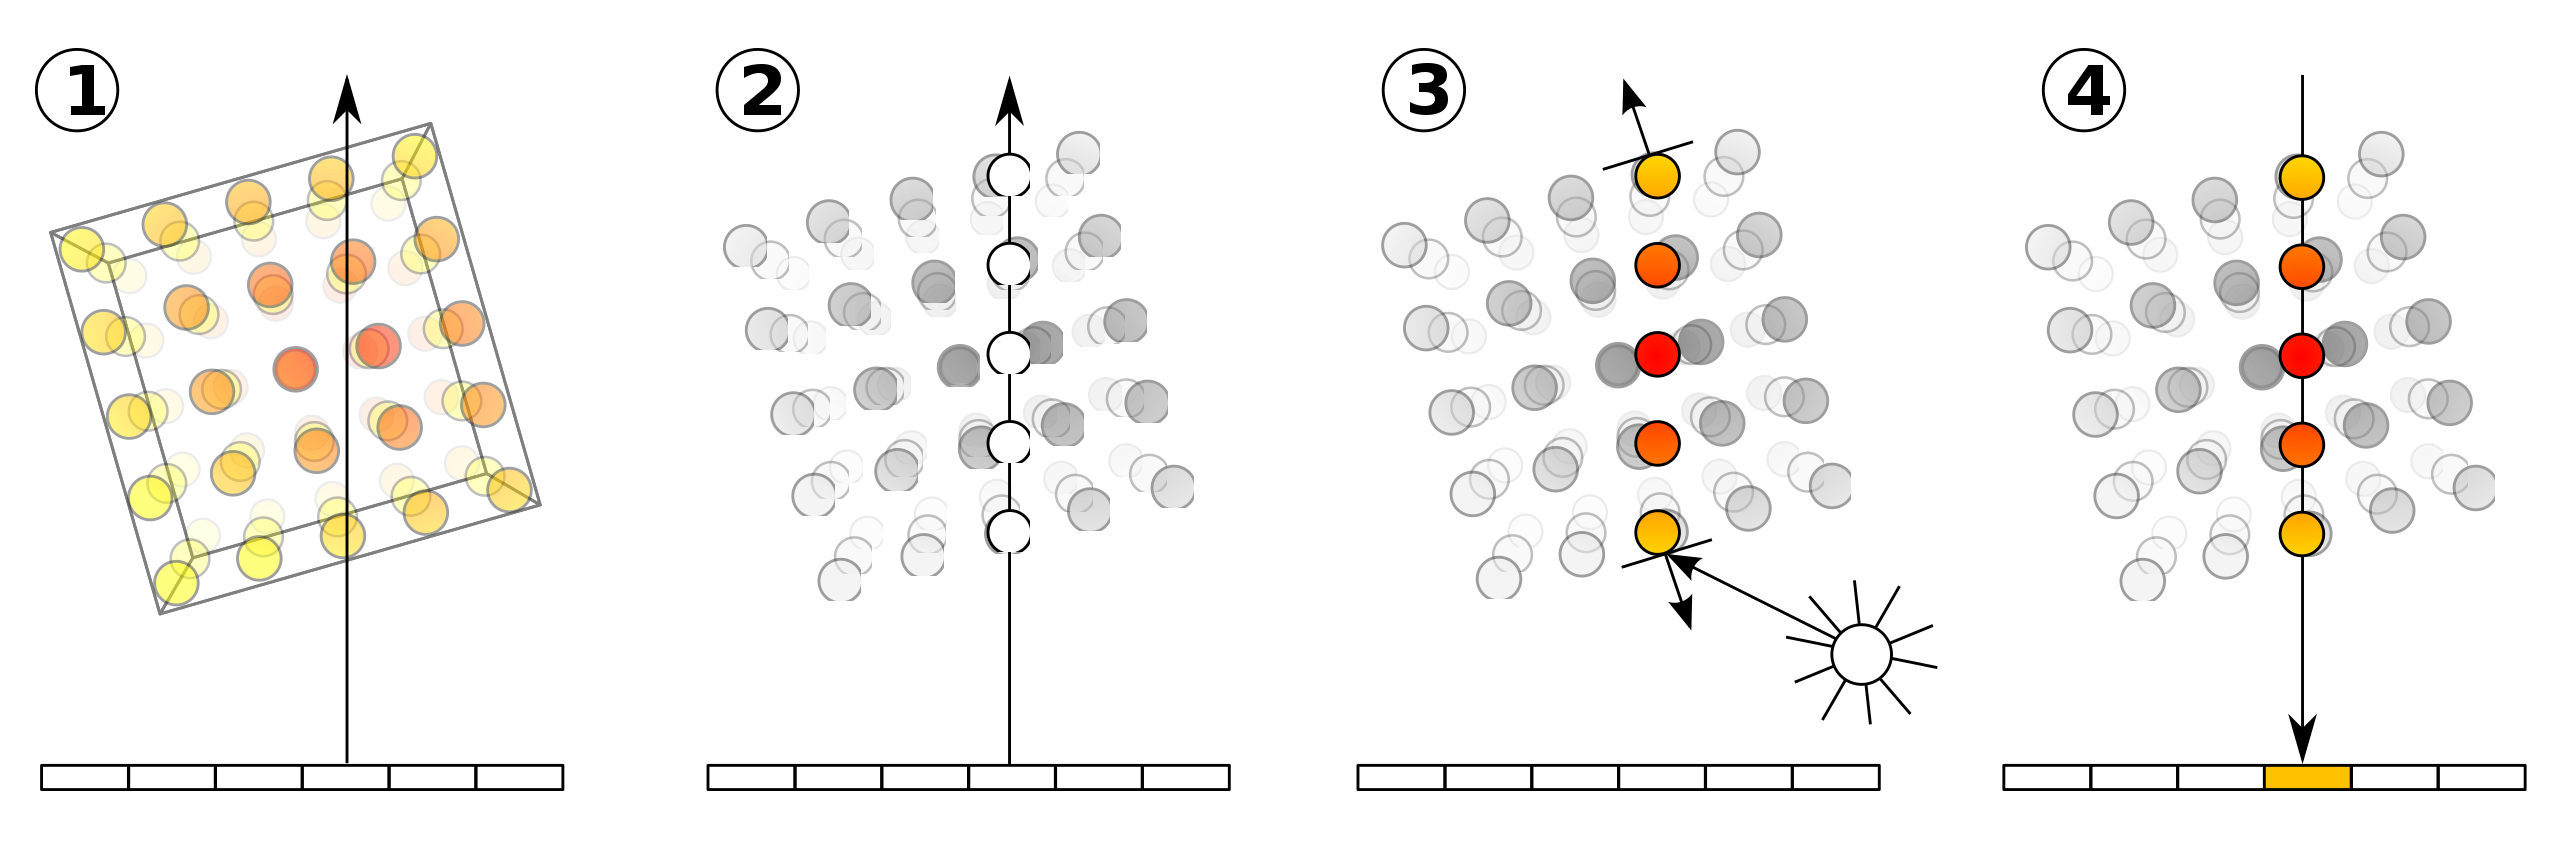
\includegraphics[width=1.0\textwidth]{figures/volume-rendering.png}
    \caption{The four basic steps of volume rendering \cite{wiki:Volume_ray_casting}. 1) A ray is cast from the image plane into the volume. 2) Points in the volume are sampled. 3) The points are shaded based on their $RGB\alpha$-value and the illumination-value gradients in relationship with the local light source. 4) The final pixel color is obtained by compositing all the shaded samples along the ray.}
    \label{fig:volume-rendering}
\end{figure}


\begin{comment}
\subsection{Alpha compositing}
Alpha compositing is the process of combining one image with a background to create the appearance of partial or full transparency \cite{wiki:Alpha_compositing}.

\subsection{Ray marching}
\end{comment}



% --------------------- Neural Fields ---------------------
\section{Neural Fields} % All text is taken from \cite{xie_neural_2022} - rewrite - have now paraphrased it
% ✅ SOMEWHAT REWRITTEN
A neural field refers to a field that has been parameterized, either entirely or partially, by an \acrfull{ann}. The field is a quantity that may be defined for any set of temporal or spatial coordinates. By design, neural fields are both continuous and adaptable. Neural fields are commonly parameterized as \acrlong{mlp}s (\acrshort{mlp}s) with gradient-defined activation functions \cite{xie_neural_2022}.

A typical neural fields algorithm in visual computing would first, across space-time, sample coordinates and feed them into an \acrshort{ann} to produce field quantities. The field quantities are samples from the desired reconstruction domain of the problem, which defines how we represent the world, such as a radiance field or another appropriate representation. Then, we apply a forward map to relate the reconstruction to the sensor domain, which defines how we observe the world, such as through an RGB image. In the sensor domain, supervision is available and we calculate the reconstruction error that guides the \acrshort{ann} optimization process by comparing the reconstructed signal to the sensor measurement. Important parts from the neural field algorithm are visualized in \autoref{fig:neural-field}.


% OLD
%A field that has been entirely or partially parameterized by a neural network is known as a neural field. The field is a quantity that may be defined for any set of temporal or spatial coordinates. By design, neural fields are both continuous and adaptable. Neural fields are commonly parameterized as MLPs with gradient-defined activation functions \cite{xie_neural_2022}.

%A typical neural fields algorithm in visual computing would first, across space-time, sample coordinates and feed them into a neural network to produce field quantities. The field quantities are samples from the desired reconstruction domain of our problem. Then, we apply a forward map to relate the reconstruction to the sensor domain (e.g. RGB image), where supervision is available. Finally, we calculate the reconstruction error or loss that guides the neural network optimization process by comparing the reconstructed signal to the sensor measurement. Important parts from the neural field algorithm are visualized in \autoref{fig:neural-field}.

\begin{figure}[!h]
    \centering
    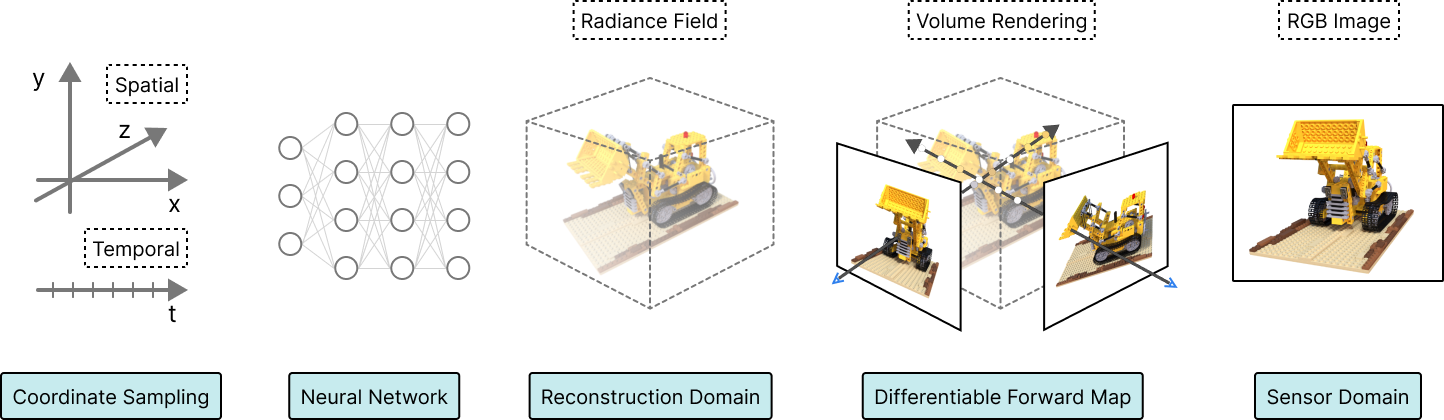
\includegraphics[width=1.0\textwidth]{figures/neural-field.png}
    \caption{Inspiration Figure 3 from Neural Fields in Visual Computing \cite{xie_neural_2022}. A typical neural fields algorithm in visual computing.}
    \label{fig:neural-field}
\end{figure}



% --------------------- Neural Radiance Fields (NeRFs) ---------------------
\subsection{Neural Radiance Fields}
% ✅ Somewhat rewritten, but mostly old.
The volumetric data we interact with through computer games, movies, and other computer graphic applications, are predominantly represented by meshes. A mesh is a collection of vertices, edges, and faces combined in order to define the shape of objects. Meshes are easy to manipulate and interact with. Another common representation of volume is voxels, where a 3D point in space is represented by a value, for example a color. Both of these modeling techniques are \textit{explicit} representations. As we want to increase the resolution of a scene, we have to model increasingly smaller regions of space, that is, increase the number of voxels/triangle-meshes in the volume. This does not scale well as the memory requirements increase as we increase the number of voxels/triangle-meshes. Due to memory constraints, we have to find another way to represent the scene, instead of representing it as explicit blocks or meshes in space. NeRF provides an \textit{implicit} representation of the scene by utilizing an \acrshort{mlp}.

NeRF is a neural volumetric representation. The name, neural radiance fields, provides a clue as to what it is. It is a field, a space full of particles, where each particle has a given radiance, a color emitted by the particle in a certain direction, and the field is represented with an \acrshort{ann}. NeRF parameterizes 3D scenes as 3D neural fields, mapping 3D coordinates to radiance and density. The 3D scene can subsequently be rendered via volume rendering, as discussed in \autoref{sec:volumerendering}.

% OLD
%Most of the volumetric data we interact with through computer games, movies, and other computer graphic applications, are represented by meshes. A mesh is a collection of vertices, edges, and faces that can be combined in order to define the shape of objects. Meshes are easy to manipulate and interact with. Another common representation of volume is voxels, where a 3D point in space is represented by a value, e.g. a color. Both of these modeling techniques are explicit representations. As we want to increase the resolution of a scene, we have to model increasingly smaller regions of space, i.e. increase the number of voxels/triangle-meshes in the volume. This doesn't scale well as the memory requirements increase as we increase the number of voxels/triangle-meshes. We have to find another way to represent the scene, instead of representing it as explicit blocks in space. NeRF provides an implicit representation of the scene by utilizing a multi-layered perceptron (MLP).

%NeRF is a neural volumetric representation. The name, neural radiance fields, gives us a clue as to what it is. It is a field, a space full of particles, where each particle has a given radiance, a color emitted by the particle in a certain direction, and the field is represented with a neural network. NeRF parameterizes 3D scenes as 3D neural fields, mapping 3D coordinates to radiance and density. The 3D scene can subsequently be rendered via volume rendering, as discussed in \autoref{sec:volumerendering}.

\subsection{Differentiable Rendering} 
NeRFs are made possible due to differentiable rendering, a major breakthrough in 3D reconstruction. Differentiable rendering enables the rendering process to be implemented in a way that is amenable to gradient-based optimization. This in turn allows for the use of techniques such as backpropagation to optimize the parameters of a scene in order to produce a desired visual result. It allows reconstruction of 3D neural fields representing shape and/or appearance given only 2D images, instead of 3D supervision. This is particularly valuable as 3D data is often expensive to obtain, while 2D images are ubiquitous. As a result, non-experts can become 3D content creators without the barrier of specialized hardware, which has important social implications \cite{xie_neural_2022}.

% Differentiable rendering enables 3D content creation from omni-present 2D images, making it accessible to non-experts without specialized hardware. This has important social implications, as 3D data acquisition is often expensive. \cite{xie_neural_2022}.

%A major breakthrough in 3D reconstruction was the adoption of differentiable rendering (Section 4), which allowed reconstruction of 3D neural fields representing shape and/or appearance given only 2D images, instead of 3D supervision. This has significant implications since 3D data is often expensive to obtain, while 2D images are omni-present. A particularly important social implication is that non-experts can become 3D content creators, without the barrier of specialized hardware. \cite{xie_neural_2022}



% --------------------- NeRF ---------------------
% ✅ Somewhat rewritten
\section[NeRF]{NeRF - Representing Scenes as Neural Radiance Fields for View Synthesis} \label{sec:nerf}
The first paper to present NeRFs was \textit{NeRF - Representing Scenes as Neural Radiance Fields for View Synthesis} \cite{mildenhall_nerf_2020}. NeRFs provide a method for reconstructing 3D scenes and synthesizing novel views. Given multiple 2D images and their corresponding camera poses, NeRF builds a dataset by sampling points in the volume. The points in the dataset are passed through an \acrshort{mlp} in order to predict the given points' density and color. The predicted density and color values are then composited into a final color which is compared to the reference image pixel's color. The \acrshort{mlp} is optimized to minimize the difference between the predicted and reference pixel color.

%NeRF does this by querying an underlying MLP overfit to a specific scene, which represents a continuous volumetric field.
%NeRF renders pixels by emitting rays into the scene. The rays are represented by the ray equation $\pmb{r}(t) = \pmb{o} + t\pmb{d}$ where $\pmb{o}$ is the ray's origin, usually the center of the camera, and $\pmb{d}$ is the ray's direction.

Given multiple 2D images and their corresponding camera poses, which can be retrieved from calibrated camera rigs or approximated with \acrshort{sfm} techniques as will be discussed in \autoref{sec:colmap}, NeRF builds a dataset by sampling points in the volume. Points are sampled along a ray $\pmb{r}(t)$ with origin $\textbf{o}$, the camera's center of projection, and viewing direction $\textbf{d}$. The sampling rate of significant parts of the volumetric scene is increased with a technique called \textit{hierarchical sampling}, which will be discussed in \autoref{sec:hierarchicalsampling}.

%Sample points along a ray $\pmb{r}(t)$, defined by the ray function \autoref{eq:ray-equation}.

\begin{equation}
    \pmb{r}(t) = \pmb{o} + t\pmb{d}
    \label{eq:ray-equation}
\end{equation}

%$\pmb{o}$ is the origin and $\pmb{d}$ is the ray's direction. 
% TODO: Make sure it's right to suffix the points with _k
Points (3D-coordinates) $\pmb{x}_k = \pmb{r}(t_k)$, where $t_k \in t$, in conjunction with their viewing direction $\pmb{d}_k$, make up the dataset in which the \acrshort{mlp} is trained on. It has been shown that MLPs have a hard time learning high-frequency signals given low-dimensional input \cite{tancik_fourier_2020}. In order to remedy this, the points are normalized to lie in the interval of $[-1, 1]$ and the signals' dimensionality is increased by applying positional encoding. The dimensionality of the points and their corresponding viewing directions are increased by applying $\gamma(\cdot)$, shown in \autoref{eq:positionalencoding}. Positional encoding will be further explained in \autoref{sec:positionalencoding}.

\begin{equation}
    \gamma(p) = [\sin(\pi p), \cos(\pi p), ..., \sin(2^{L-1}\pi p), \cos(2^{L-1}\pi p)]^T
    \label{eq:positionalencoding}
\end{equation}

A predicted color can be obtained by passing the encoded 3D coordinate and its corresponding encoded camera pose through the \acrshort{mlp} denoted $F_{\theta}$, where $\theta$ represents the network parameters. The output of $F_\theta$ is a 4D vector containing a color $RGB$ and a density $\sigma$. In order to retain multiview consistency, NeRF first predicts the volume density $\sigma$ as a function of only the location $\textbf{x}$. Subsequently, the RGB color $\pmb{c}$ is predicted as a function of both the location and viewing direction.


Using the points' density $\sigma$ and color $\pmb{c}$ we can approximate the volume rendering, as discussed in \autoref{sec:volumerendering}, to synthesize a novel view of the scene. The expected color $C(\pmb{r})$ can be derived by \autoref{eq:volume-rendering}, which further can be approximated with numerical quadrature as shown in \autoref{eq:numerical-quadrature-loss}.

%Feed $\gamma(x)$ and its corresponding encoded camera pose given by $\gamma(\theta)$ and $\gamma(\phi)$ into the MLP $F_{\theta}$

\begin{equation}
    C(r) = \int_{t_n}^{t_f}T(t)\sigma(\pmb{r}(t))\pmb{c}(\pmb{r}(t), \pmb{d})dt \quad T(t) = \exp{\left(-\int_{t_n}^{t_f}\sigma(\pmb{r}(s))ds\right)}
    %C(r) = \int_{t_n}^{t_f}T(t)\sigma\pmb{c}dt \quad T(t) = \exp{(-\int_{t_n}^{t_f}\sigma ds)}
    \label{eq:volume-rendering}
\end{equation}
\begin{align} \label{eq:numerical-quadrature-loss}
    \hat{C}(\pmb{r}) = \sum_{i=1}T_i \alpha_i \pmb{c}_k, && \text{where}~T_i &= \exp{(-\sum_{j=1}^{i-1} \sigma_j \delta_j)},  \\ 
    && \alpha_i &= (1-e^{-\sigma_i}), \\ 
    && \delta_i &= t_{i+1} - t_i
\end{align}

The transmittance $T(t)$ represents the probability that the ray will not intersect any objects up to point $t$. $\sigma(\pmb{r}(t))$ and $c(\pmb{r}(t), \pmb{d})$ represents the density and color of point $\pmb{r}(t)$, respectively.

Since volume rendering is differentiable, we optimize the loss between the synthesized and ground truth observed image. This is done by calculating the total squared error between the ground truth pixel colors $C(\pmb{r})$ and the synthesized pixel color $\hat{C}(\pmb{r})$ over all the rays $\pmb{r} \in \mathcal{R}$. This loss is called the \textit{photometric loss}. Both the coarse and fine networks, subscripted with $c$ and $f$ respectively and later elaborated upon in \autoref{sec:hierarchicalsampling}, are optimized over.

\begin{equation}
    L = \sum_{\pmb{r} \in \mathcal{R}} \left[\left\| \hat{C}_c(\pmb{r}) - C(\pmb{r}) \right\|^2_2 + \left\| \hat{C}_f(\pmb{r}) - C(\pmb{r}) \right\|^2_2\right]
    \label{eq:nerf-loss}
\end{equation}

% ✅ Somewhat rewritten
\subsubsection{Positional Encoding} \label{sec:positionalencoding}
Positional encoding is one of the many proposed encoding schemes, first introduced in the original NeRF paper. It is a method used to increase the dimensionality of an input vector, as it is shown that deep networks are biased toward learning lower-frequency functions. It is important to note that positional encoding in the context of NeRF is distinct from the positional encoding employed in transformers.

% ✅ Rewritten
\subsubsection{Stratified sampling} \label{sec:stratifiedsampling}
Stratified sampling is a sampling method that has proven benefits in machine learning as it helps prevent overfitting. The sampling method can be broken into three steps:

\begin{itemize}
    \item \textbf{Partition the dataset into strata}: In the case of NeRF, the rays are partitioned into equally sized bins where the points contained within a bin $\pmb{x} \in [t_i, t_i+1]$ along the ray $\pmb{r}(t)$, comprises the respective stratum.
    \item \textbf{Determine the number of samples to take from each stratum}: The sample size from a stratum can vary based on predefined functions. Importance sampling can be achieved by increasing the sample size in accordance with a \acrshort{pdf}.
    \item \textbf{For each stratum, apply simple random sampling}: Simple random sampling is applied to each stratum to select a predefined number of points randomly and with equal probability.
\end{itemize}

\begin{figure}[h]
    \centering
    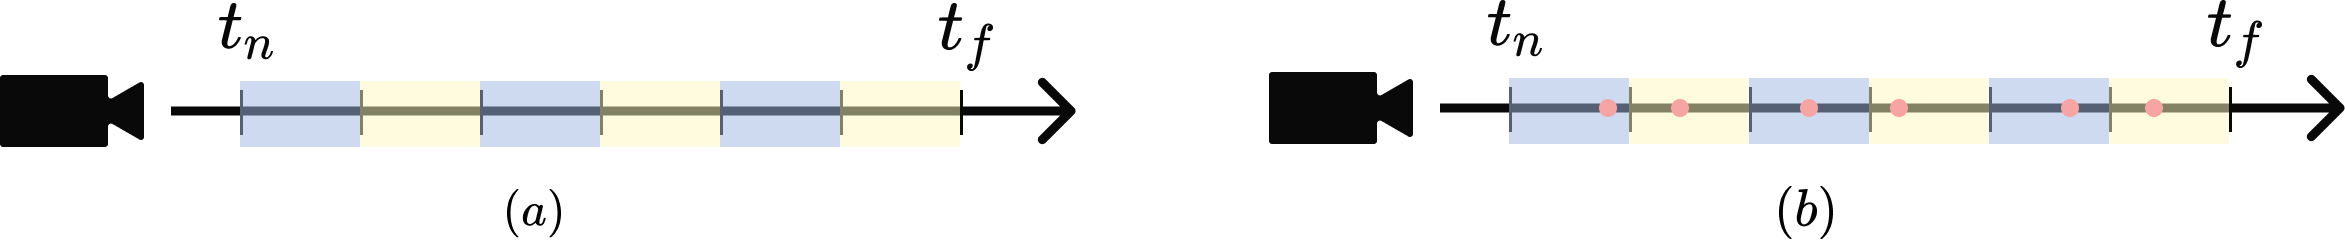
\includegraphics[width=1.0\textwidth]{figures/stratified-sampling.png}
    \caption[Stratified sampling]{a) The ray is uniformly binned from the near bound $t_n$ to the far bound $t_f$, defining the strata. b) A single random point is randomly sampled from each stratum.}
    \label{fig:stratified-sampling}
\end{figure}

% ✅ Somewhat rewritten
\subsubsection{Hierarchical sampling} \label{sec:hierarchicalsampling}
When training a NeRF, different sampling strategies can be utilized. The sampling strategy is an important choice as it is core to how the dataset for the \acrshort{mlp} is constructed. The original NeRF paper \cite{mildenhall_nerf_2020} proposed the use of a sampling approach called hierarchical sampling. This method involves training two MLPs: a \textit{coarse} \acrshort{mlp} and a \textit{fine} \acrshort{mlp}. During training, the coarse \acrshort{mlp} employs stratified sampling which involves uniform interval sampling within each bin along the ray. The coarse \acrshort{mlp} outputs a \acrfull{pdf} that highlights the samples that significantly contribute to the final predicted RGB value. This \acrshort{pdf} is then passed to the fine \acrshort{mlp} which sample points along the ray in accordance with the \acrshort{pdf}. This strategy of having a coarse network predict the important areas to sample, that is the regions containing volume, facilitates the fine network in generating improved predictions.

% Point from Mip-NeRF 360. Doesn't fit very well here, but it's a good point!
%The only reason why the coarse network is supervised is to guide the sampling of the fine network. This is the motivation behind improvements in e.g. Mip-NeRF 360



An overview of the NeRF pipeline can be viewed in \autoref{fig:nerf-pipeline}

\begin{figure}[h]
    \centering
    %\hspace*{-48px}
    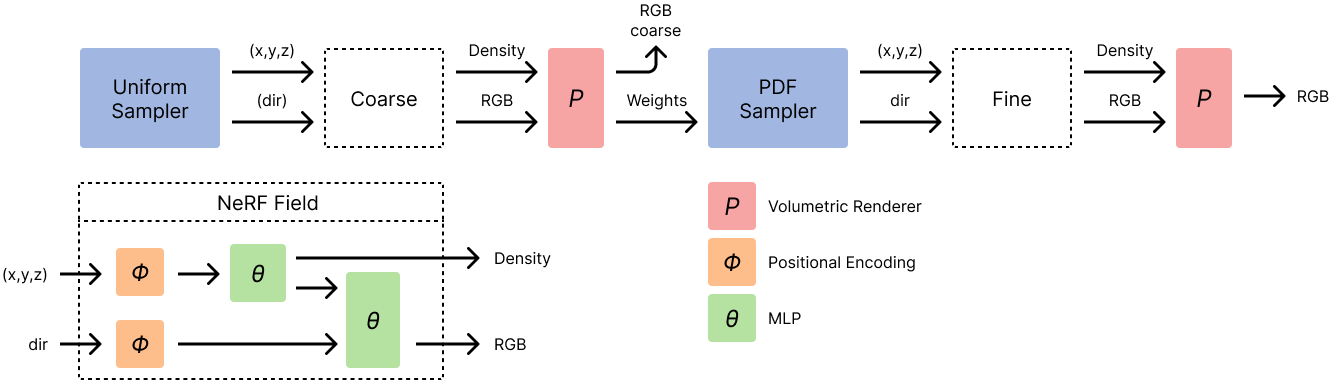
\includegraphics[width=1.0\textwidth]{figures/nerf-pipeline-overview.png}
    \caption{Overview of the NeRF pipeline}
    \label{fig:nerf-pipeline}
\end{figure}


% --------------------- Structure from motion ---------------------
\section{COLMAP (Structure from Motion)} \label{sec:colmap}
% ✅ Rewritten
\acrshort{sfm} is a technique for estimating 3D structures from sequences of 2D input images. Although some NeRF approaches have  endeavored to eliminate the necessity for pose supervision \cite{lin_barf_2021}\cite{wang_nerf--_2022}, accurate camera poses are typically a strict requirement in most NeRF methods. As a result, SfM techniques may be employed as a preprocessing mechanism for retrieving the camera poses of the input images.

% TODO: Add section about how BaRF and NeRF-- both only work on object-centric scenes.

% OLD
%Structure from motion is a technique for estimating 3D structures from sequences of 2D input images. In NeRF it can be used as a preprocessing tool for retrieving camera poses of the input images. In most NeRF methods, accurate camera poses are a strict requirement, although some papers have experimented with removing the need for pose supervision \cite{lin_barf_2021}\cite{wang_nerf--_2022}.

% ❌ Pretty happy with how this reads. Haven't changed anything
%\subsection{COLMAP} \label{sec:colmap}
COLMAP is a general-purpose SfM \cite{schonberger_structure--motion_2016} and \acrfull{mvs} \cite{schoenberger2016mvs} pipeline. The general overview of the pipeline contains the following steps:
\begin{enumerate}
    \item Feature detection and extraction
    \item Feature matching and geometric verification
    \item Structure and motion reconstruction
\end{enumerate}

During the first step, \acrfull{sift} \cite{lowe_distinctive_2004} is used to extract features in the images. This algorithm finds sparse feature points in the image and describes their appearances using numerical descriptors.

% TODO: Elaborate on the different match-options; Exhaustive Matching, Sequential Matching, Vocabulary Tree Matching. Runtimes, found in the paper, can be added to appendix.

During the second step, features are matched. Correspondences between the feature points are matched across different images, leveraging feature matching and geometric verification. There are different options for matching algorithms. \textit{Exhaustive matching} would match every image against every other image, leading to the best reconstruction results. The time complexity is not an issue if the number of images is relatively low (several hundreds). Another option is \textit{sequential matching} which is useful if the captured images are in sequential order, for example, if they are sampled from a video.

During the third step, structure and motion is reconstructed. First, COLMAP will generate a sparse reconstruction of the scene, extracting the camera poses (camera extrinsics). The sparse output serves as input to the \acrshort{mvs} to recover a dense representation of the scene. The dense representation estimates the dense surfaces. In NeRF-applications, COLMAP is primarily used as a preprocessing step for retrieving the camera poses of input images. Because of this, the pipeline is usually ceased after the sparse reconstruction.

\begin{table}[h] 
\centering
\begin{tabular}{lcc}
\hline
Matching algorithm & \multicolumn{1}{l}{Time complexity} & \multicolumn{1}{l}{Space complexity} \\ \hline
Exhaustive         & $\mathcal{O}(n^2)$       & $\mathcal{O}(n^2)$  \\
Sequential         & $\mathcal{O}(n k)$ & $\mathcal{O}(n k)$        \\
Vocabulary Tree    & $\mathcal{O}(n^2)$       & $\mathcal{O}(n k)$  \\ \hline
\end{tabular}
\caption[Time and memory complexities of COLMAP matching algorithms.]{An overview of the time and memory complexities of a selection of COLMAP matching algorithms. For sequential matching $k$ is the number of adjacent images each image $n$ is matched against. For Vocabulary tree-based matching, $k$ is the number of top-retrieved images that each image $n$ is matched against.}
\label{tab:colmap-feature-complexity}
\end{table}

\begin{comment}
Exhaustive matching:
time complexity: O(n^2), where n is the number of images
memory complexity: O(n) for storing all images, O(n^2) for storing the results of the matching process

Sequential matching:
time complexity: O(n * k), where n is the number of images and k is the number of adjacent images each image is matched against
memory complexity: O(n * k)

Vocabulary tree-based matching:
time complexity: O(n^2), assuming that the size of the vocabulary tree is constant and not a function of the number n of images
memory complexity: O(n * k), where k is the number of top-retrieved images that each image is matched against
There is definitively literature on the topic of the time and memory complexity of vocabulary tree-based matching and image retrieval
\end{comment}

\section{Nerfstudio} \label{sec:nerfstudio}
%Since publication of the original NeRF paper, a multitude of different methods regarding NeRF has been published. Some of the papers are published with corresponding source code and some not. However, it's no easy task to compare the different methods on self-captured data. Nerfstudio is an open-source framework/API that 

Since the publication of the original NeRF paper \cite{mildenhall_nerf_2020}, a multitude of different methods regarding NeRF has been published. With the magnitude of published methods, some with corresponding source code and some not, it is not trivial to compare them on self-captured data. Nerfstudio \cite{nerfstudio} is an open-source framework/API that streamlines the process, training, evaluation, and rendering of NeRFs. The components that make up NeRFs are modularized in a way that allows interpretable implementation of different NeRF methods. In addition, Nerfstudio ships with implemented versions of some of the most important published methods to date for real-world captures. The core concepts within Nerfstudio are presented in \autoref{fig:nerfstudio-pipeline-components}. 

\begin{figure}[!h]
    \centering
    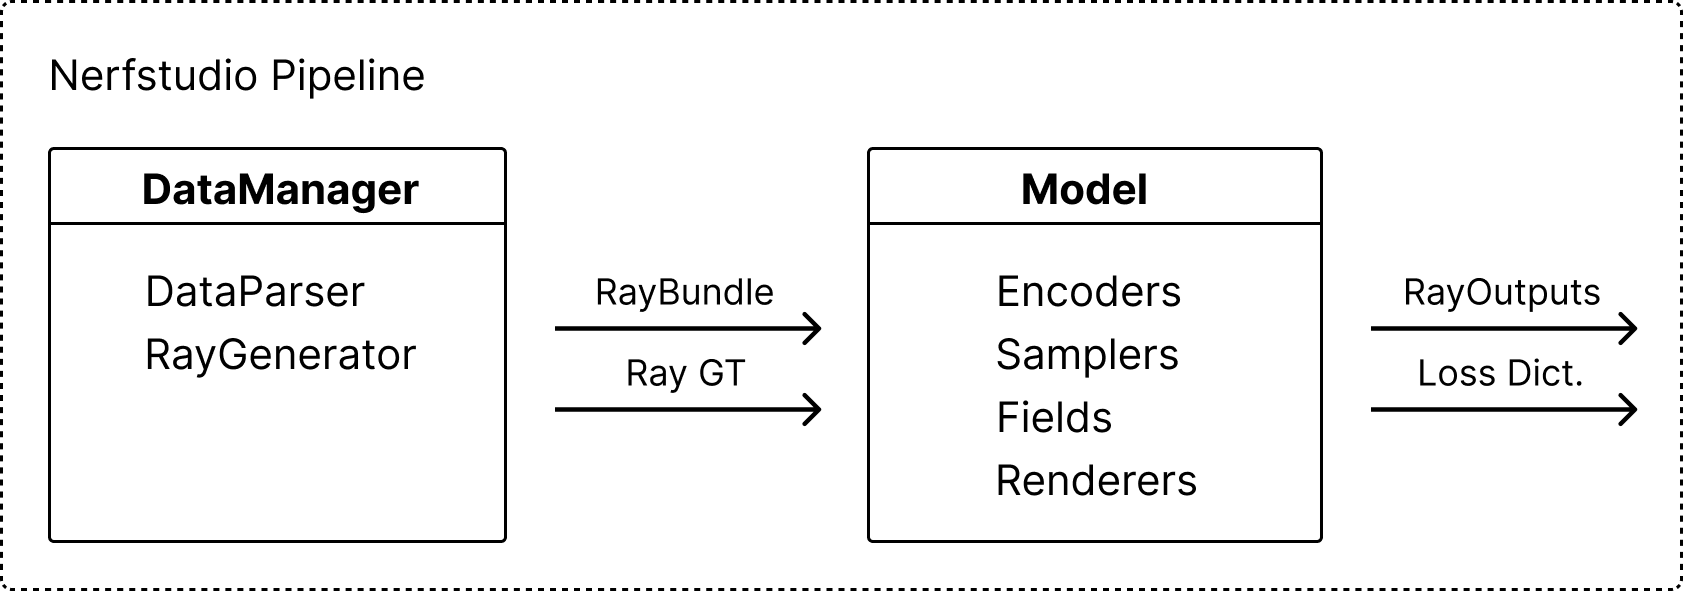
\includegraphics[width=1.0\textwidth]{figures/nerfstudio-pipeline-components.png}
    \caption[The components of the Nerfstudio pipeline.]{The components of the Nerfstudio pipeline. \texttt{DataManager}s process input images into bundles of rays (\texttt{RayBundles}) that are rendered by the \texttt{Model} to produce a set of NeRF outputs (\texttt{RayOutputs}). A dictionary of losses supervises the pipeline. Figure and caption adapted from Figure 2 in \textit{Nerfstudio: A Modular Framework for Neural Radiance Field Development} \cite{tancik_nerfstudio_2023}.}
    \label{fig:nerfstudio-pipeline-components}
\end{figure}

%\textbf{\texttt{DataManagers} and \texttt{DataParsers}}:



\section{CARLA} \label{sec:carla}
CARLA \cite{Dosovitskiy17} is an open-source simulator for \acrshort{ad} research which enables the capture of synthetic data in a controllable and programmable environment. Its highly customizable simulation environment allows for the creation and testing of a wide range of driving scenarios and conditions. CARLA includes a variety of sensors, such as cameras, \acrfull{lidar}, and \acrfull{gps}/\acrshort{gnss}, which can be used to collect both visual and non-visual data. We can interact with the CARLA simulator via a Python API, which allows for the control of vehicle position, orientation, and most other behaviors within the simulation. This flexibility enables the generation of diverse and realistic data, making CARLA, among many other things, a powerful tool for the development and testing of data capture pipelines. Data captured from CARLA can be seen in \autoref{fig:carla-3-camera-setup}.

\begin{figure}[ht]
    \centering
    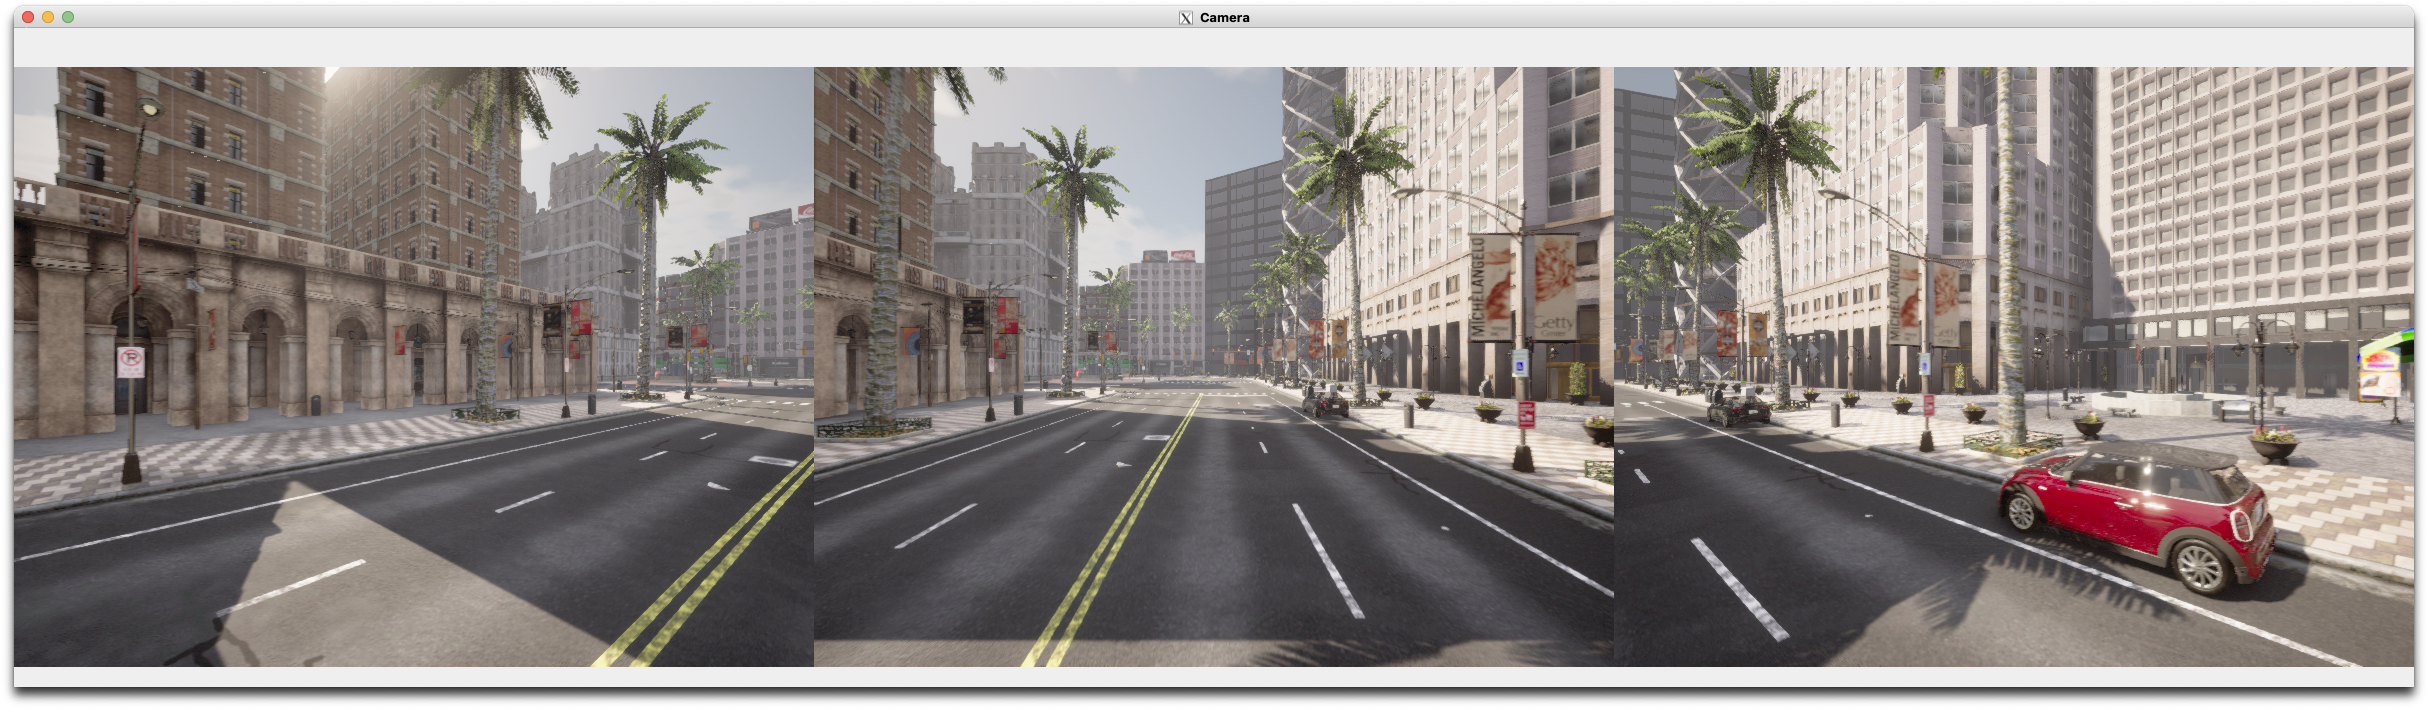
\includegraphics[width=1.0\textwidth]{figures/carla-3-camera-setup.png}
    \caption[Screenshot from the CARLA simulator.]{A screenshot from a simulation in the CARLA environment where a car has been equipped with three cameras with different rotations. The output from the mounted cameras have been horizontally stacked and rendered with OpenCV\cite{opencv_library}.}
    \label{fig:carla-3-camera-setup}
\end{figure}



% --------------------- Evaluating NeRFs ---------------------
% ✅ Rewritten
\section{Evaluating NeRFs} \label{sec:evaluating-nerfs} 
Evaluating the quality of NeRFs is a difficult task due to the visual nature of the modality. Once a NeRF is trained, it is typically employed to render an image, making image similarity metrics the most critical measure for evaluating NeRF quality. The evaluation of image similarity has been a persistent challenge in computer graphics, but the following metrics are commonly used throughout most papers comparing NeRFs.

% OLD
% Evaluating the quality of NeRFs is inherently hard since it's a visual modality. After a NeRF is trained it will eventually be used to render an image. Image similarity metrics are consequently the most important metric to evaluate the quality of a NeRF. The assessment of image similarity has been a long-standing challenge in computer graphics, but the following metrics are commonly used throughout most papers comparing NeRFs.

% ✅ Not much done, already well-written subsection.
\subsection[PSNR]{\acrfull{psnr}} \label{sec:psnr}
\acrshort{psnr} is a common measure for quantifying reconstruction quality for images and videos. It builds upon \acrfull{mse} which measures the absolute difference between each pixel in two images $I_1$ and $I_2$.

\begin{align} 
    \text{PSNR} &= 20 \cdot \log_{10}\left(\dfrac{MAX_I}{\sqrt{\text{MSE}}}\right) \label{eq:psnr}, \ \text{where} \\ 
    %\\ &= 20 \cdot log_{10} (MAX_I) - 10 \cdot log_{10}(MSE)
    \text{MSE} &= \dfrac{1}{m n} \sum_{i = 0}^{m-1} \sum_{j = 0}^{n-1} \left[I_1(i,j) - I_2(i, j) \right]^2, \ \text{and} \label{eq:mse}
\end{align}

and $MAX_I$ represents the dynamic range of an image; the largest range of pixel values that the picture may contain. This is 255 when pixels are represented with 8 bits per sample. In more general terms, $MAX_I$ is $2^B-1$ when samples are recorded with $B$ bits per sample. Due to the high dynamic range of many signals, \acrshort{psnr} is typically expressed as a logarithmic number using the \acrfull{db} scale.


% ✅ Rewritten
\subsection[SSIM]{\acrfull{ssim}}
While \acrshort{mse} and \acrshort{psnr} are effective measures of reconstruction error, they do not evaluate an image in the same manner as humans. Rather than comparing pixel values in order to conclude if two images are similar, humans assess images holistically. \acrshort{ssim} attempts to replicate this approach by comparing an image's luminance $l$, contrast $c$, and structure $s$ between two windows $\pmb{x}$ and $\pmb{y}$ of a common size $N \times N$.

% OLD
%Although MSE and PSNR are good measures of the reconstruction error, they don't examine an image the same way humans do. We don't compare pixel-value to pixel-value in order to conclude if two images are similar, we look at it in a more holistic way. SSIM tries to capture this by instead comparing luminance $l$, contrast $c$ and structure $s$ between two windows $x$ and $y$ of common size $N \times N$.

\begin{align} \label{eq:ssim}
    \text{SSIM}(x, y) &= l(x,y)^\alpha \cdot c(x,y)^\beta \cdot s(x,y)^\gamma \qquad \text{with } \alpha, \beta, \gamma = 1 \\
    &= \dfrac{(2\mu_x \mu_y + c_1)(2\sigma_{xy} + c_2)}{(\mu_x^2 + \mu_y^2 + c_1)(\sigma_x^2 + \sigma_y^2 + c_2)}
\end{align}

\begin{comment}
\begin{itemize}
    \item $\mu$ represents the pixel sample mean for both $x$ and $y$,
    \item $\sigma^2$ represents the variance for both $x$ and $y$,
    \item $\sigma_{xy}$ represents the covariance of x and y,
    \item $c_1 = (k_1L)^2$, $c_2 = (k_2L)^2$ are variables to stabilize the division with weak denominator,
    \item $L$ represents the dynamic range of the pixel-values,
    \item $k_1 = 0.01$, $k_2 = 0.03$ by default   
\end{itemize}
\end{comment}

\acrshort{ssim} is bounded by $-1 \leq \text{SSIM} \leq 1$ where $1$ implies perfect correlation, $0$ implies no similarity, and $-1$ implies perfect anti-correlation.


% ✅ Rewritten
\subsection[LPIPS]{\acrfull{lpips}}
\acrshort{lpips} \cite{zhang_unreasonable_2018} is a perceptual similarity metric based on deep network activations. Unlike \acrshort{mse}, \acrshort{psnr} and \acrshort{ssim} which uses relatively shallow functions in order to determine similarity across images, \acrshort{lpips} leverages deep neural networks to obtain a metric that perceives similarity in a way that is similar to humans. 

The dataset used to train \acrshort{lpips} includes two types of perceptual judgments; \acrfull{2afc} and \acrfull{jnd}. In \acrshort{2afc}, people were asked to select which of two distorted images was “closer” to the reference, while in \acrshort{jnd}, people were presented with two image patches, one reference and one distorted, and asked if they were the same. Some samples from the dataset is depicted in \autoref{fig:lpips}. By training on this dataset, \acrshort{lpips} is able to capture higher-level features of images that are more relevant to human perception, such as object shapes and textures. This makes it a more effective similarity metric than traditional metrics like \acrshort{mse}, \acrshort{psnr}, and \acrshort{ssim}. Image patches with a low \acrshort{lpips} score are perceptually similar.

\begin{figure}[ht]
    \centering
    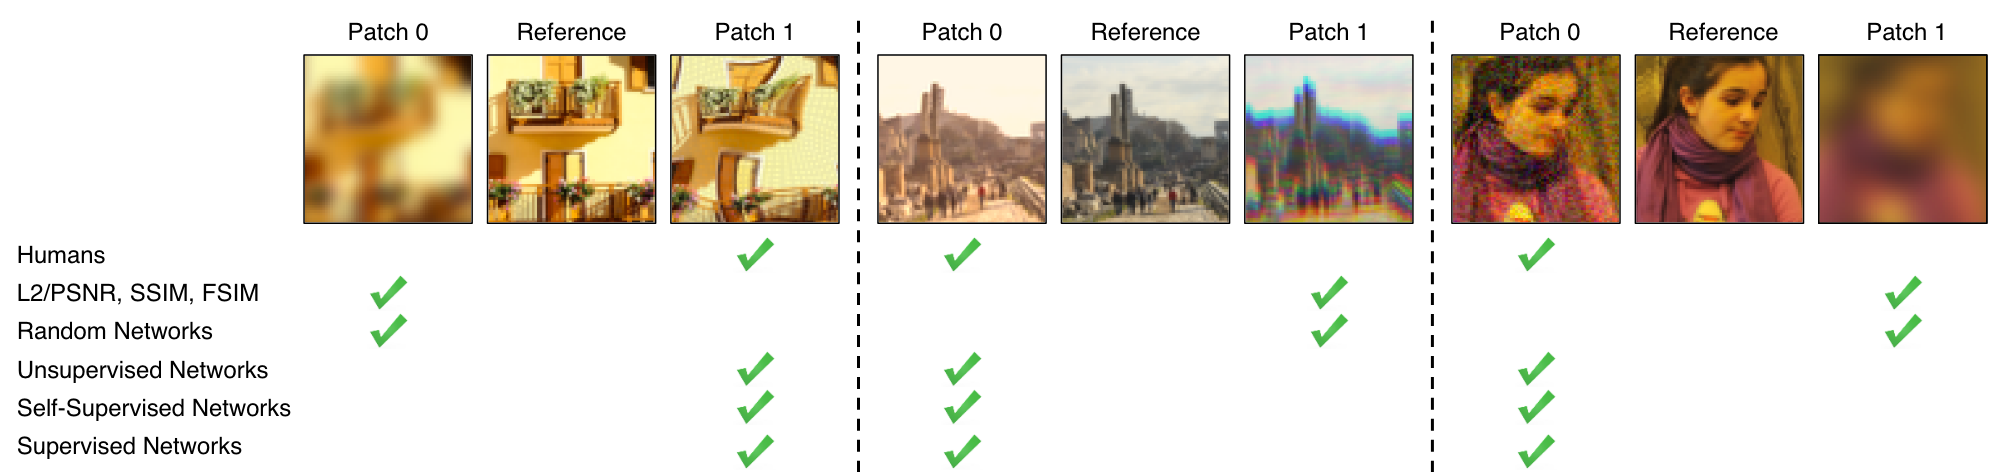
\includegraphics[width=1.0\textwidth]{figures/lpips.png}
    \caption[LPIPS - Learned Perceptual Image Patch Similarity]{\acrshort{lpips} is trained to perceive image similarity the same way humans do. The dataset used to train the similarity metric contains two types of perceptual judgements, \acrshort{2afc} and \acrshort{jnd}. With \acrshort{2afc} people were asked to select which of the distorted images was "closer" to the reference. With \acrshort{jnd} people were presented with 2 image patches, one reference and one distorted, and asked if they were the same. Figure 1 from \acrshort{lpips} \cite{zhang_unreasonable_2018}.}
    \label{fig:lpips}
\end{figure}



%The metric determines how similar two image patches' activations are, for a given network. It's been demonstrated that this metric closely matches human perception. Image patches with a low LPIPS score are perceptually similar.


\section{Related Work}
% --------------------- Other models that Nerfacto builds on ---------------------
Since the publication of the original NeRF paper, there has been a surge of related papers proposing new methods, techniques, and applications. This section covers some of the significant NeRF methods, including more specific work on the application of NeRF on vehicle-captured data.

% --------------------- mip-NeRF ---------------------
\subsection[Mip-NeRF]{Mip-NeRF: A Multiscale Representation for Anti-Aliasing Neural Radiance Fields} \label{sec:mipnerf}
NeRF demonstrates impressive performance when the training and evaluation images are captured at similar distances from the scene, without the need to account for scale or aliasing effects. When you add more cameras, pulled away from the scene, NeRF starts to deteriorate because it is a single-scale model now trying to solve a multi-scale problem. As a consequence, renderings from the NeRF exhibit aliasing artifacts in distant views and excessive blur in close-up views.

A solution to this problem would be to adopt a technique that is used in offline ray tracing, \textit{supersampling}. With supersampling, we would march multiple rays through the same pixel's footprint. This technique does not resolve the issue of aliasing effects, but it does result in improved visual quality of the rendered image. However, doing so would be very computationally expensive and it would further increase the lengthy training times of NeRF, which already relies on querying an underlying \acrshort{mlp} hundreds of times for a single ray.

Another sampling strategy apart from casting rays through each pixels' footprint would be to cast a cone, as seen in \autoref{fig:mip-nerf-frustums}. The cone's radius is determined by the size of the pixel's footprint on the image plane, thereby enabling the cone to model the whole volume of space visible by the pixel. When the pixel's cone is rendered, all the content within that visible volume will be averaged out, instead of rendering out whatever intersects with the infinitely narrow ray cast by NeRF. The cone is divided into conical \textit{frustums}. The frustums are approximated with a multivariate Gaussian since they are easier to manipulate and have a closed-form solution.

Instead of positionally encoding a single point along the ray, we compute the expected positional encoding with respect to the 
constructed Gaussian. With this encoding, Mip-NeRF is able to reason about the scale of its input by analyzing the scale of the encodings. This allows the model to understand the difference between small and large volumes. This encoding scheme is called \acrfull{ipe}, and has a simple closed-form solution that can be computed quickly.

\begin{figure}[ht]
    \centering
    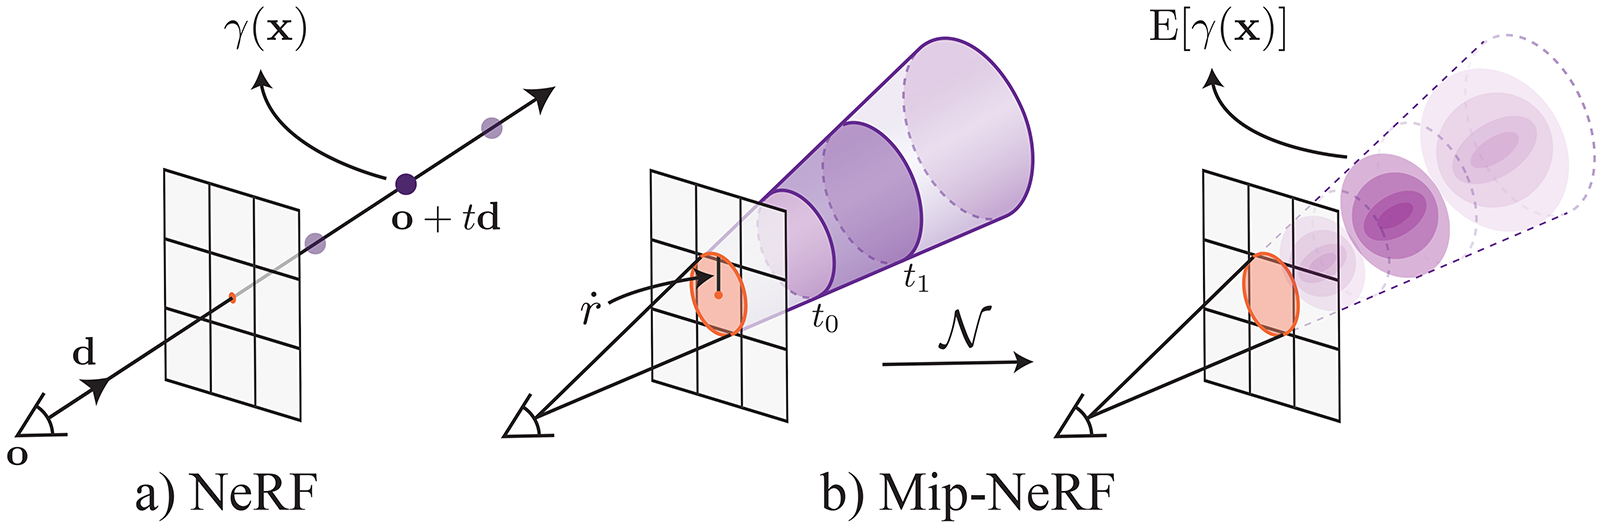
\includegraphics[width=1.0\textwidth]{figures/mip-nerf-frustums.png}
    \caption[Illustration of positional encoding]{A comparison of sampling strategies. NeRF (a) samples points along rays traced through each pixel before positionally encoding the points. Mip-NeRF (b) cast cones through the pixels' footprint and into the volume before applying \acrfull{ipe}. Figure 1 from Mip-NeRF \cite{barron_mip-nerf_2021}.}
    \label{fig:mip-nerf-frustums}
\end{figure}

This method draws inspiration from mipmapping \cite{williams1983pyramidal}, a technique traditionally used in computer graphics pipelines to mitigate aliasing artifacts. Mipmapping involves generating a pre-filtered set of discretely downsampled signals, typically images, which accelerates rendering by shifting the responsibility of anti-aliasing to a pre-computation phase. Mip-NeRF extends NeRF to simultaneously represent the pre-filtered radiance field for a continuous space of scales, thereof "Mip-NeRF".

\autoref{fig:mip-nerf-pipeline-overview} provides an overview of the Mip-NeRF pipeline. The primary distinction from the NeRF pipeline, as depicted in \autoref{fig:nerf-pipeline}, is the incorporation of the Mip-NeRF field, which utilizes \acrshort{ipe}.

\begin{figure}[h]
    \centering
    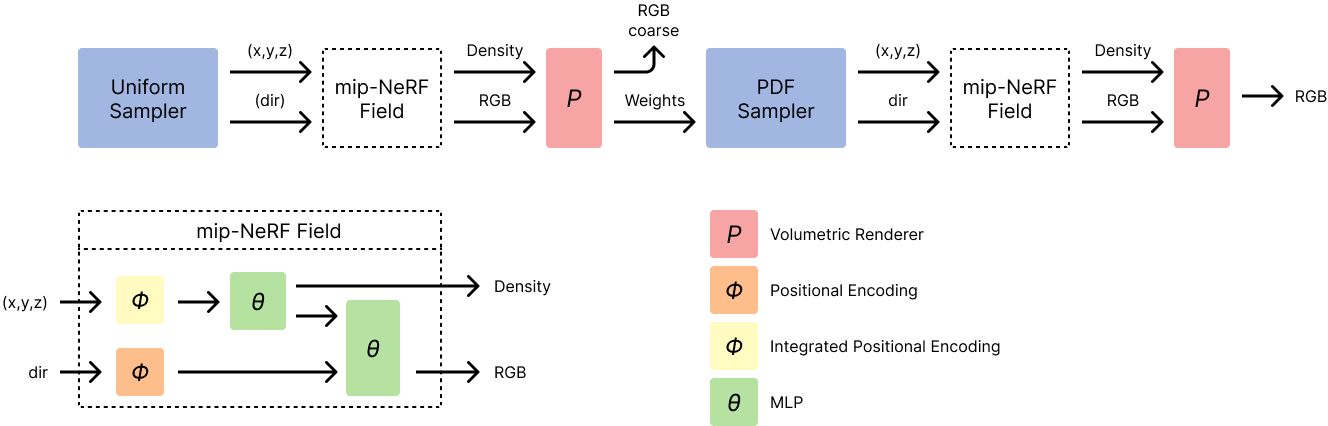
\includegraphics[width=1.0\textwidth]{figures/mip-nerf-pipeline-overview.png}
    \caption{Overview of the Mip-NeRF \cite{barronMipNeRFMultiscaleRepresentation2021} pipeline.}
    \label{fig:mip-nerf-pipeline-overview}
\end{figure}



% --------------------- mip-NeRF 360 ---------------------
\subsection[Mip-NeRF 360]{Mip-NeRF 360: Unbounded Anti-Aliased Neural Radiance Fields} \label{sec:mipnerf360}
Mip-NeRF introduces several valuable techniques for advancing the capabilities of NeRFs. However, the techniques are primarily focused on forward-facing scenes \cite{mildenhall2019llff} as opposed to unbounded scenes that are object-centric, featuring elaborate backgrounds and images captured from $360^\circ$ around the object. To extend the capabilities of Mip-NeRF to unbounded scenes, Mip-NeRF 360 \cite{barron_mip-nerf_2022} proposes three primary techniques, which are covered in this subsection.

\subsubsection{Representation}
%Problem: Unbounded scenes are large, but mip-NeF needs a bounded domain
%Solution: Apply a Kalman-like warp to mip-NeRF Gaussians to warp the mip-NeRF into non-Euclidean space.
The first challenge with extending Mip-NeRF to unbounded scenes is that such scenes are large, but Mip-NeRF requires a bounded domain. Mip-NeRF handles scenes unbounded in one direction by warping the space into \textit{projective space}, \acrfull{ndc}, but the challenge arises when the scene is unbounded in all directions. A solution is to apply a Kalman-like warp to Mip-NeRF Gaussians in order to warp the Mip-NeRF into non-Euclidean space. All the Gaussians outside a sphere of radius one will smoothly be warped into a non-euclidean space within a sphere of radius two. This non-Euclidean space is used to represent the input to the \acrshort{mlp}. 


\subsubsection{Efficiency}
%Problem: Large scenes require more network capacity, but using a large MLP is too expensive (given that you have to query it hundred of times for a single ray)
%Solution: "Distill" scene geometry from a large NeRF MLP into a small MLP while training. Train a small proposal MLP to bound the geometry predicted by a large NeRF MLP which makes training ~3 times faster
Expanding a bounded scene to an unbounded scene results in larger scenes that require a more substantial network capacity. However, using a large \acrshort{mlp} is too expensive given that it has to be queried hundreds of times for a single ray. A solution is to distill scene geometry from a large NeRF \acrshort{mlp} into a small \textit{proposal MLP} while training. The proposal \acrshort{mlp} will only output a set of weights, no colors. By feeding a set of location points through the proposal \acrshort{mlp}, the outputted weights can then be used as a \acrshort{pdf} to resample the ray, similar to how the coarse network in hierarchical sampling guides the fine network's sampling. The resampled points are then used to render a color, which as normal is supervised with photometric loss. Rather than supervising the proposal \acrshort{mlp} to accurately reconstruct the image, which is done for both the coarse and fine MLPs in Mip-NeRF, the output weights are supervised to be consistent with the output weights from the NeRF \acrshort{mlp}. This is accomplished using a loss function that encourages the outputted weight histograms to be consistent with one another. This is made possible with some strong assertions on the relation between the two distributions, which ultimately summarizes the same underlying and true distribution. This new approach to training accelerates training speeds by 300\%.

%i.e. calculate a loss that correlates the output weights from the NeRF MLP and the proposal MLP. Due to this we can have a very small proposal MLP which we query very frequently, and a larger NeRF MLP which is queried relatively few times.
%To make this work we need a loss function that encourages histograms with different bin endpoints to be consistent with one another. To achieve this we make some strong assertions on the relation between the two distributions, summarizing the same underlying, true distribution. The loss function will penalize any excess mass that violates the upper bound imposed on the proposal MLP.


\subsubsection{Ambiguity}
%Problem: 3D reconstruction becomes more ambigious as you increase the scene size. Results in more artifacts
%Solution: Utilize a novel regularizer designed specifically for mip-NeRF ray intervals. The regularizer encourages each ray's histogram to be as close to a delta function as possible. 
Reconstructing 3D content from 2D photos is inherently ambiguous since the content of unbounded scenes can be everywhere and will only be seen by a tiny number of rays. This problem becomes more pronounced as scene size increases. The original NeRF-paper partially addressed this behavior by introducing random Gaussian noise to the output $\sigma$ values, before passing them through the \acrfull{relu} \cite{agarap_deep_2019}. This stimulated densities to drift toward either zero or infinity, which slightly enhanced visual performance. However this regularization is insufficient for the more challenging task that Mip-NeRF 360 tackles. Instead, Mip-NeRF 360 introduces a novel regularizer, specifically designed for Mip-NeRF ray intervals, that encourages each ray's histogram to be as close to a delta function as possible. This regularizer reduces the occurrences of "floaters", which are semi-transparent objects that appear to be floating in space.

\begin{figure}[!h]
    \centering
    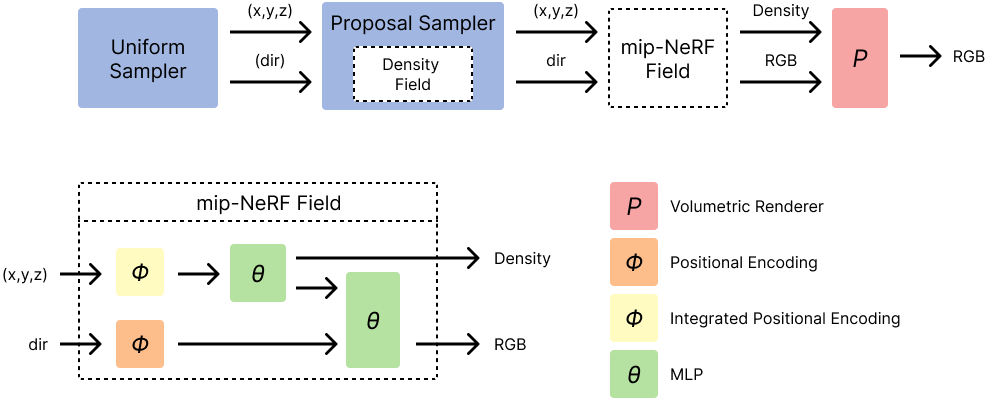
\includegraphics[width=1.0\textwidth]{figures/mip-nerf-360-pipeline-overview.png}
    \caption{Overview of the mip-NeRF 360 pipeline}
    \label{fig:mip-nerf-360-pipeline-overview}
\end{figure}

\autoref{fig:mip-nerf-360-pipeline-overview} provides an overview of the Mip-NeRF 360 pipeline, which differs in several respects from the previous Mip-NeRF pipeline depicted in \autoref{fig:mip-nerf-pipeline-overview}. Notably, the pipeline does not render a redundant RGB value, and instead features two distinct fields: a density field and a Mip-NeRF field.


\subsection[Block-NeRF]{Block-NeRF: Scalable Large Scene Neural View Synthesis} \label{sec:block-nerf}
Block-NeRF \cite{tancik_block-nerf_2022} is a paper that demonstrates a method for reconstructing large-scale scenes using NeRFs. This is achieved by splitting large areas into multiple blocks of a certain radius, with each block having a connected NeRF referred to as a Block-NeRF. The different Block-NeRFs are trained on images within their respective radius of responsibility. At inference time, only the Block-NeRFs with a radius that spans the requested location are kept. These have all been trained on image data from the requested location and can render an output. Some of the remaining Block-NeRFs might still lack a direct line of sight to the requested location, which results in low "visibility", which will be discussed further in \autoref{sec:visibility-prediction}. These Block-NeRFs are also filtered out, resulting in a pool of Block-NeRFs with good visibility. The remaining Block-NeRFs render the given location, and their outputs are merged to render the final image output.

Block-NeRF leverages multiple techniques in order to enable the reconstruction of large scenes. These include \textit{appearance embeddings}, \textit{learned pose refinement} and \textit{visibility prediction}.

\subsubsection{Appearance embeddings} \label{sec:appearance-embeddings}
Per-image appearance conditioning is a technique that was first proposed for NeRFs in NeRF\nobreakdash-W \cite{martin-brualla_nerf_2021} and has since been employed in multiple other methods. The appearance embeddings help reduce artifacts in the scene, especially "ghosting" artifacts which present themselves as fog in the final render. The appearance embedding is a vector in a low-dimensional space, unique for every input image, that is optimized jointly with the NeRF in order to allow the NeRF to process and represent 3D scenes with variable lighting, exposures, weather, and post-processing effects. To account for these variations, the final part of the \acrshort{mlp} is conditioned by passing the viewing direction concatenated with the appearance embedding.
%The appearance embedding is concatenated with the viewing direction and passed through an MLP 

\subsubsection{Learned pose refinement} \label{sec:camera-pose-refinement}
Camera pose refinement is a technique that has been proposed to alleviate the strict requirement for accurate camera poses in NeRF. This is accomplished by treating the camera poses and intrinsics as learnable parameters and jointly optimizing them with the 3D scene representation, that is, optimizing both the photometric loss and the corresponding camera poses. It was proposed for forward-facing scenes in \textit{NeRF\nobreakdash-\nobreakdash-} \cite{wang_nerf--_2022} and later built upon in \textit{BaRF} \cite{lin_barf_2021} to support the use on object-centric scenes. Block-NeRF leverages this technique on a per-driving-segment basis. Although it is a technique optimized for forward-facing and object-centric scenes, Block-NeRF demonstrates the technique's efficacy in reducing cloudy artifacts and increasing the sharpness and overall quality of the resulting 3D representation.


\subsubsection{Visibility prediction} \label{sec:visibility-prediction}
Visibility prediction is performed to predict whether a given point is within the line of sight of a specific Block-NeRF. The prediction is made by a secondary \acrshort{mlp} $F_v$ that is trained to learn an approximation of the visibility of a sampled point. Given a location and a viewing direction, $F_v$ outputs an approximation of that location's transmittance ($T$ in \autoref{eq:volume-rendering}). The transmittance of a location will be close to 1 if it is visible, that is, if it is located in free space or on the surface of the first intersected object. Objects inside or behind the first intersected object will have a transmittance close to 0. If the point is visible from multiple viewing directions, the resulting transmittance will be the average of these observations. $F_v$ is supervised by the Block-NeRF's main \acrshort{mlp} $F_\sigma$.



% --------------------- Instant-ngp ---------------------
\subsection[Instant-ngp]{Instant-ngp: Instant Neural Graphics Primitives with a Multiresolution Hash Encoding} \label{sec:instant-ngp}
Instant-ngp \cite{muller_instant_2022} is a paper that introduces a method for accelerating the training- and inference of NeRFs. Previous NeRF methods have required hours or even days of training to learn a scene, but the team at Nvidia was able to significantly reduce both the training- and inference time while maintaining the same level of quality. This achievement represented a significant advancement in the field of NeRFs, and has greatly improved the efficiency and effectiveness of NeRF-based applications.

\begin{figure}[H]
    \centering
    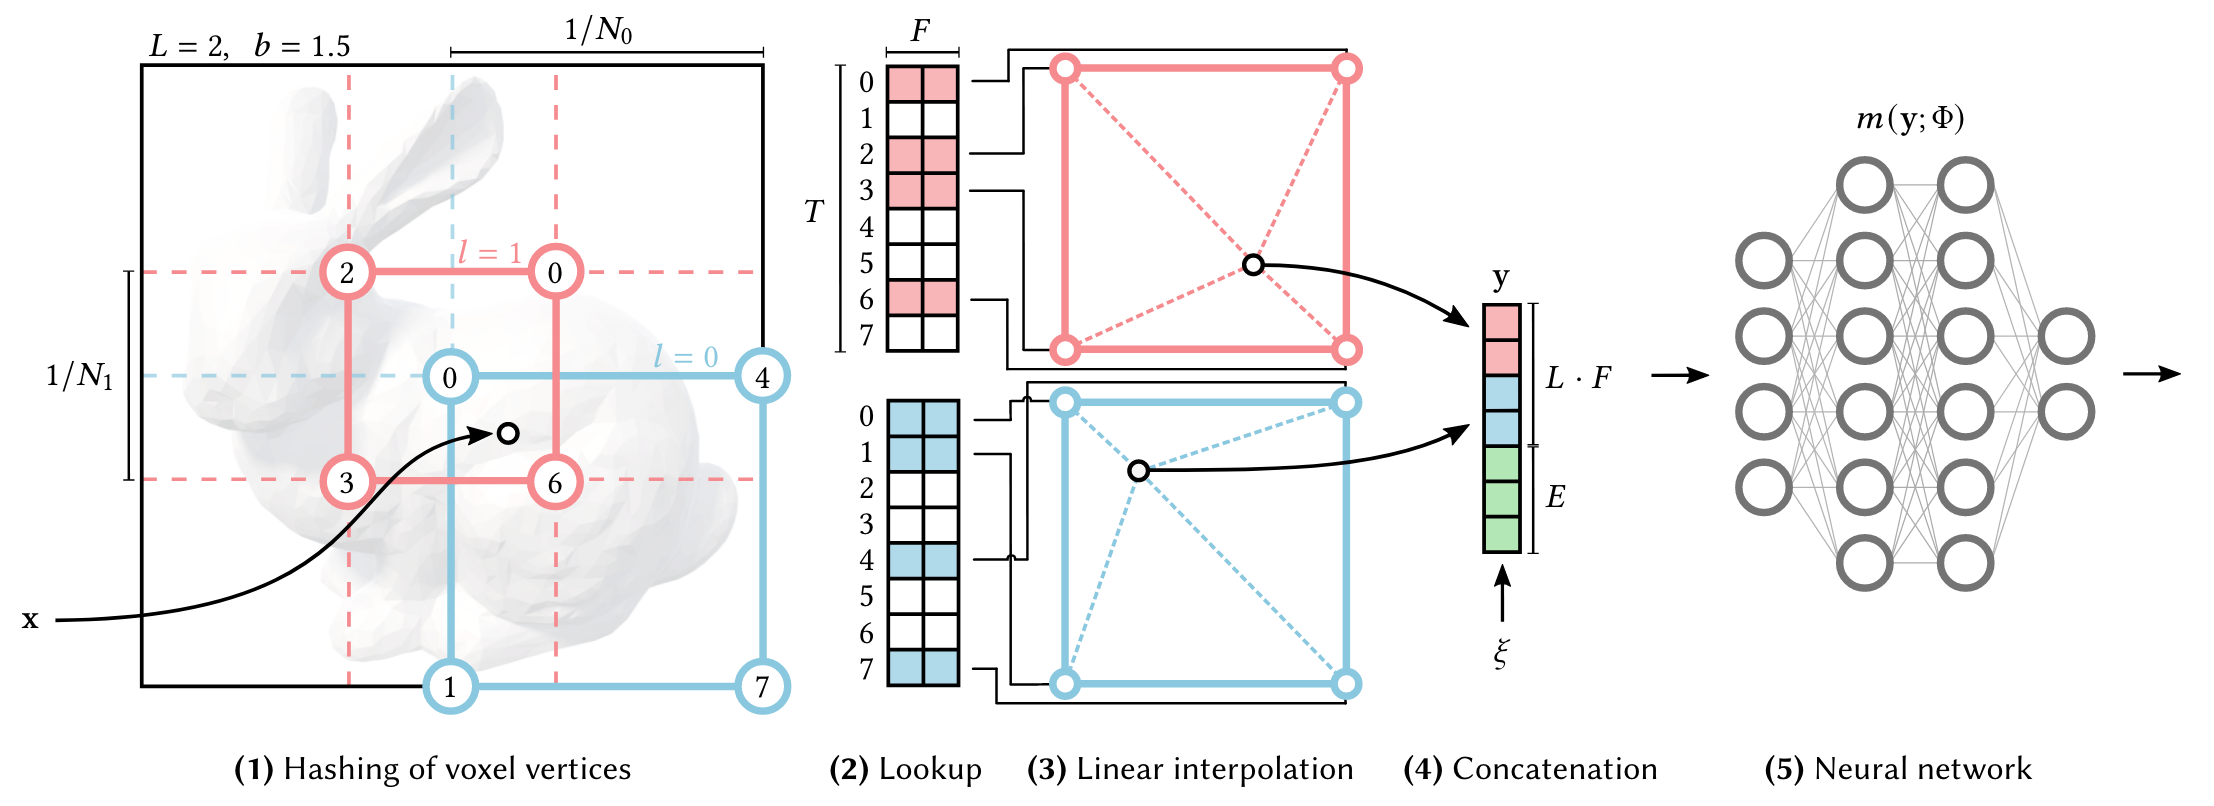
\includegraphics[width=1.0\textwidth]{figures/instant-ngp-hash-encoding.png}
    \caption[Illustration of multiresolution hash encoding]{Illustration of the multiresolution hash encoding in 2D. Figure 3 from Instant-ngp \cite{muller_instant_2022}.}
    \label{fig:instant-ngp-hash-encoding}
\end{figure}

The main technique proposed by Instant-NeRF is a new parametric encoding for the scene's spatial data, coined \textit{Multi-resolution hash encoding}. In the original NeRF paper, the location \textbf{x} is represented by a positional encoding as described in \autoref{sec:positionalencoding}. With the multiresolution hash encoding, the location \textbf{x} is represented in a hash table by a linear interpolation of its closest vertices at multiple resolutions. This parametric encoding has several advantages in terms of computational effectiveness, resulting in several magnitudes of increased training and inference speed. Although a larger memory cost is imposed by allocating several hash tables, the number of required parameter-updates per backpropagation is significantly reduced. An overview of the multiresolution hash encoding can be seen in \autoref{fig:instant-ngp-hash-encoding}.

%The only difference is essentially how spatial data is represented, i.e. parametric encoding. Instant-NGP encodes spatial data at multiple resolutions using hash tables, thereof the name multiresolution hash tables. During backpropagation, the MLP's weights and the feature vectors in the hash tables are both updated.
%In a fully connected MLP, every weight and bias must be updated on back-propagation. With parametric encodings, only a very small number of feature vectors must be updated. Also, by reducing the size of the MLP, such parametric models can be trained to convergence much faster without sacrificing approximation quality. You trade a larger memory footprint by allocating hash tables, but in return you have to update a far lower number of trainable parameters per back-propagation, leading to an increased training and inference speed.

\subsection{Nerfacto} \label{sec:nerfacto}
Nerfstudio, discussed in \autoref{sec:nerfstudio}, also provides its own method dubbed Nerfacto \cite{tancik_nerfstudio_2023}. Nerfacto leverages techniques from several other published methods that have proved to work well for real data capture. The combination of techniques, partially depicted in \autoref{fig:nerfacto-pipeline-overview}, results in a method that strikes a great balance between quality and speed. 
The primary techniques implemented in Nerfacto have already been discussed. However, they will be briefly listed and summarized in this section:

\begin{figure}[!h]
    \centering
    %\hspace*{-48px}
    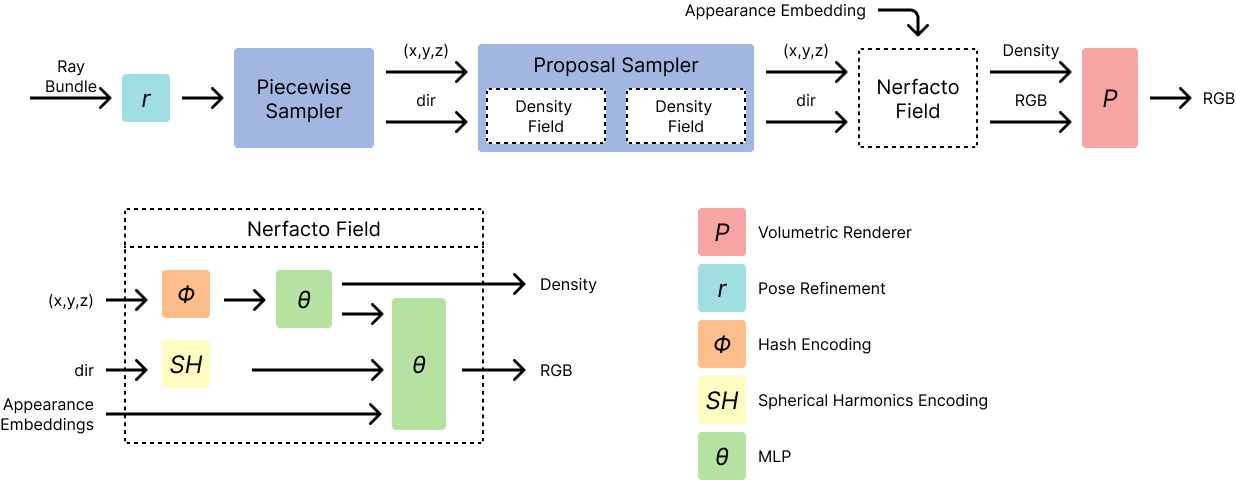
\includegraphics[width=1.0\textwidth]{figures/nerfacto-pipeline-overview.png}
    \caption{Overview of the Nerfacto pipeline}
    \label{fig:nerfacto-pipeline-overview}
\end{figure}

\textbf{Camera pose refinement}, as described in \autoref{sec:camera-pose-refinement} is a technique proposed to reduce the impact of imperfect camera poses. It is an effective measure to reduce cloudy artifacts and increase the sharpness and overall quality of the resulting 3D representation.

\textbf{Per image appearance conditioning}, as described in \autoref{sec:appearance-embeddings}, is a technique that allows the NeRF to process and represent 3D scenes with variable lighting, exposures, weather, and post-processing effects. In Nerfacto, the appearance embedding is a vector of size 32, which is concatenated with the viewing direction before it is passed through the \acrshort{mlp}.

\textbf{Hash encodings}, as described in \autoref{sec:instant-ngp}, is an effective encoding scheme used to severely decrease training- and inference time. In Nerfacto, 16 hash tables with $2^{19}$ rows, each storing a feature vector of size 2, are allocated. The subsequent \acrshort{mlp} has a very low capacity, with only one hidden layer containing 64 neurons.

\textbf{Proposal sampling}, as described in \autoref{sec:mipnerf360}, is a sampling technique used to increase the sampling density of areas that contribute most to the final render. Nerfacto extends the proposal sampler used in Mip-NeRF 360 \cite{barron_mip-nerf_2022} by utilizing two density functions implemented as small fused-\acrshort{mlp} with hash encodings \cite{muller_instant_2022}. This provides accurate and fast density estimations.

\textbf{Scene contraction}, as described in \autoref{sec:mipnerf360}, is a technique proposed in Mip-NeRF 360 \cite{barron_mip-nerf_2022} to extend Mip-NeRF to support unbounded scenes.




\subsection[Wayve - NeRFs for Autonomous Driving]{Wayve - Building City-Scale Neural Radiance Fields for Autonomous Driving} \label{sec:wayve}
Wayve, a London-based company, is a leading innovator in \acrshort{ad} technology. At Nvidia GTC, they presented a talk on how they leverage NeRFs to extend their pipeline used to train autonomous vehicles. Their initial need was a simulator that was indistinguishable from reality, but building such a simulator is very time-consuming, challenging, and expensive. Their solution was to use NeRFs to automatically "build the simulator with data."

The pipeline, partially depicted in \autoref{fig:wayve-pipeline}, begins by creating a large corpus of data, captured by a specialized Wayve-vehicle fitted with high-quality cameras. The corpus is then split into data segments spanning roughly 100 meters and containing a small overlap between the previous and successive segments. In order to mask out transient objects and separate foreground and background, a segmentation model is applied to each segment. After this, each segment utilizes COLMAP to approximate the images' corresponding camera poses. Once the camera poses are acquired, each of the NeRFs are trained in parallel with an undisclosed method. Using the capture trajectory, a camera path is created and rendered by swapping NeRFs on-demand when the current camera within the path is close to another NeRF's boundary. 

\begin{figure}[!h]
    \centering
    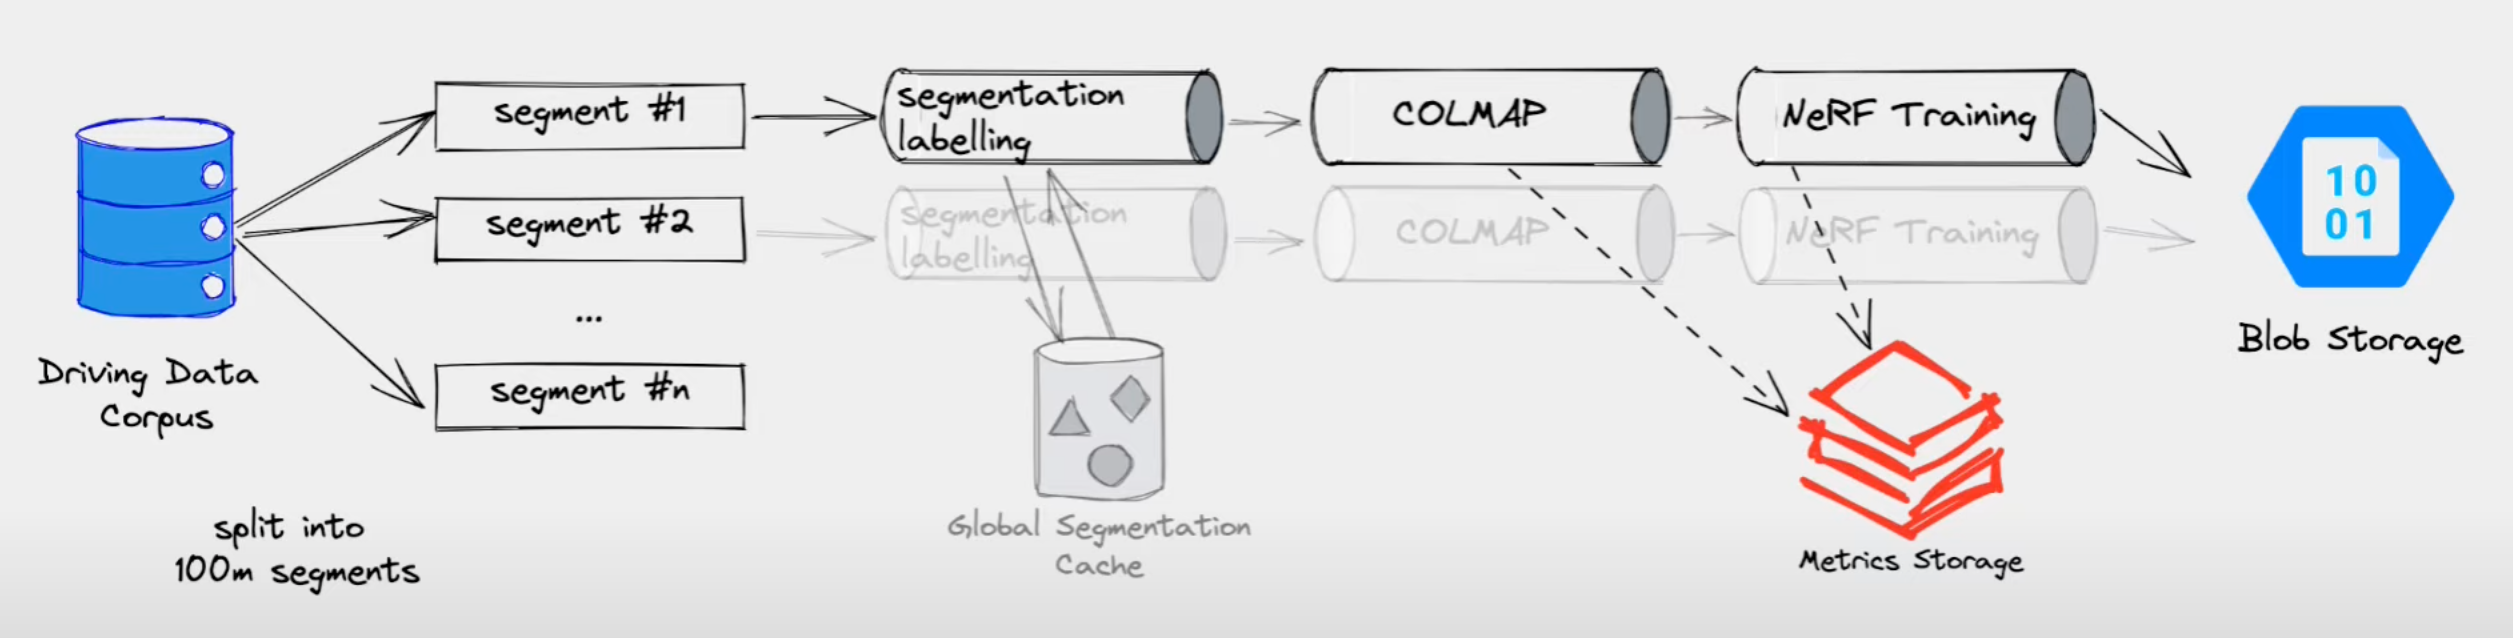
\includegraphics[width=1.0\textwidth]{figures/wayve-pipeline.png}
    \caption{An overview of Wayve's pipeline for large-scale NeRF. Image taken from Wayve's talk at Nvidia GTC \cite{sokolski2023building}.}
    \label{fig:wayve-pipeline}
\end{figure}

Wayve's pipeline is simpler and more straightforward than that of Block-NeRF because their goal is to stitch together scenes that were recorded one after the other, rather than creating a scene that can be traversed in all directions. This difference in objective allows Wayve to sidestep many of the technicalities involved in Block-NeRF making their pipeline more streamlined.
\chapter{Methods}
%The method chapter of this paper describes the process from creating a data capture pipeline, extending it to a full end-to-end capture-to-render pipeline with Nerfstudio, using the pipeline to create a data capture baseline, using the baseline to run further experiments, extending the baseline to support large scale scenes, and finally extending it to support real data.

This chapter is split into multiple parts, all essential for the end-to-end pipeline, depicted in \autoref{fig:end-to-end-pipeline}, to allow the capture of data and subsequent training, evaluation, and render of a NeRF with Nerfstudio. The separate components are thoroughly explained.

% TODO: Write that we're going to use Nerfstudio here?

\begin{figure}[ht]
    \centering
    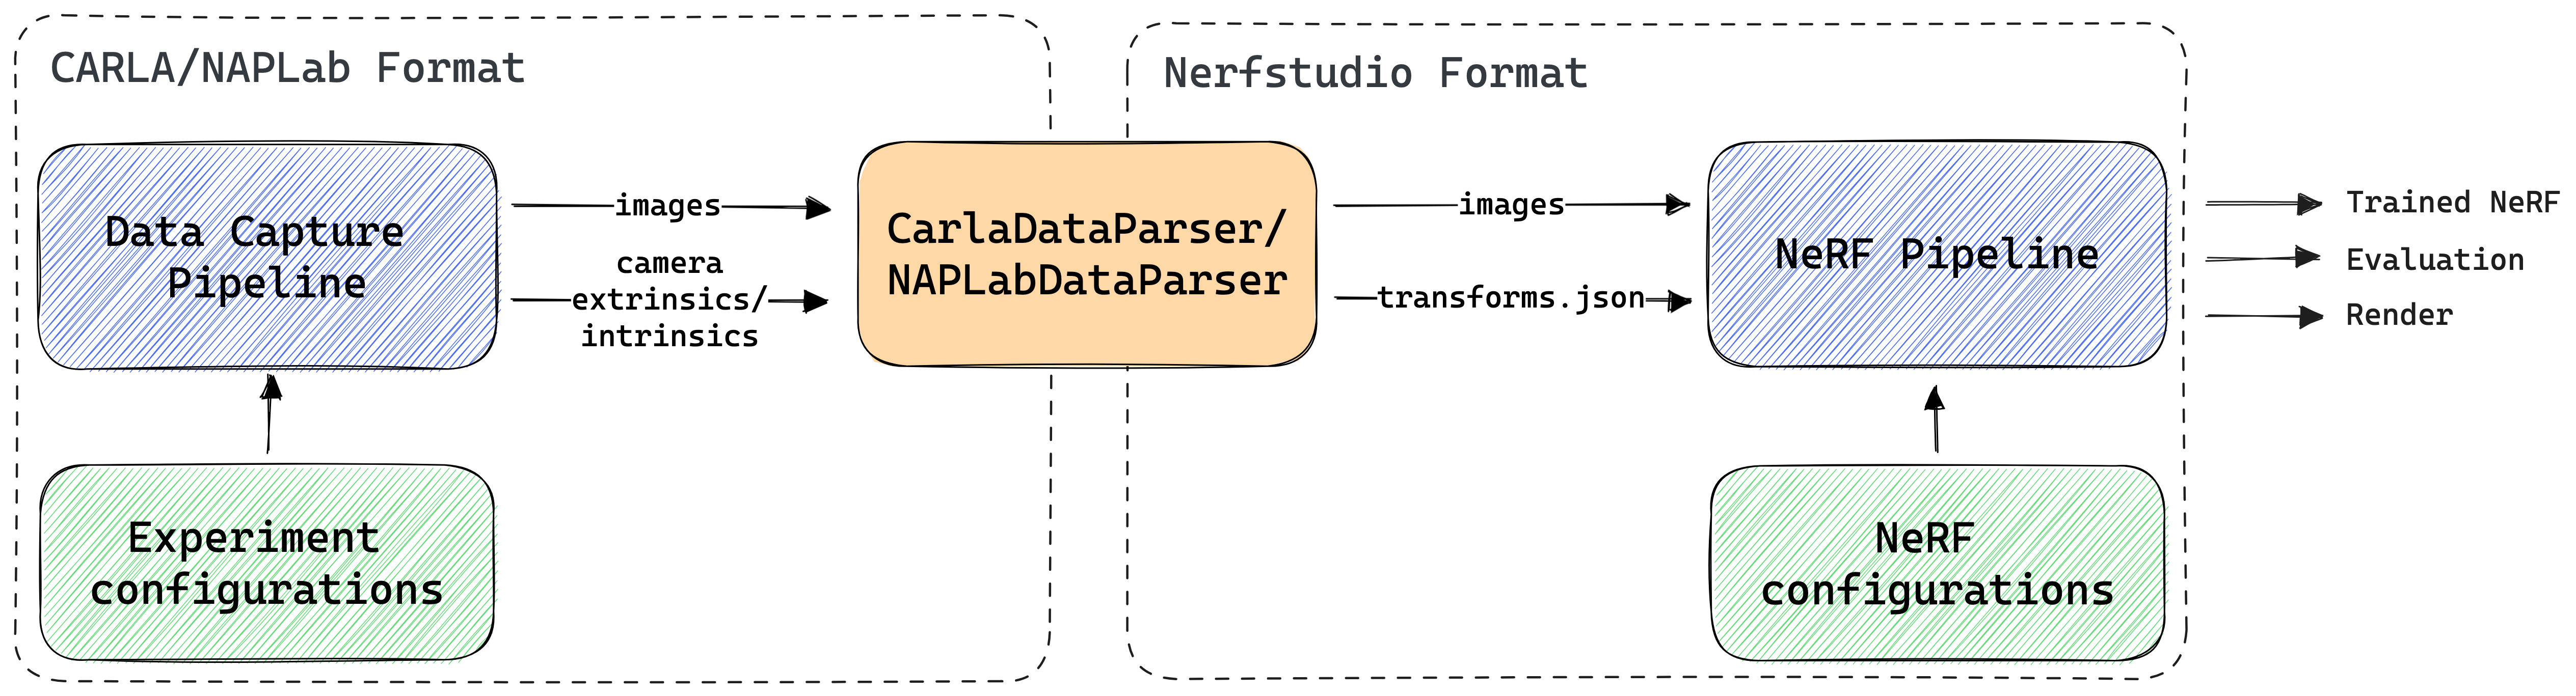
\includegraphics[width=1.0\textwidth]{figures/end-to-end-pipeline-v2.png}
    \caption[Overview of the end-to-end pipeline.]{Overview of the end-to-end pipeline that captures data from CARLA or the \acrshort{naplab} car, converts the data into Nerfstudio format, and utilizes the resulting data to train, evaluate, and render a camera path for the NeRF.}
    \label{fig:end-to-end-pipeline}
\end{figure}

\begin{comment}
This chapter elucidates the methodological approach employed in this research to explore the potential of Neural Radiance Fields (NeRF) in improving the synthetic data pipeline from CARLA to Nerfstudio. Our approach is underpinned by a systematic series of stages, each contributing to the robustness of the pipeline, and enabling us to establish a baseline leveraging synthetic data from CARLA.

We start this chapter by detailing the process of collecting synthetic data from CARLA, a sophisticated platform for generating artificial datasets. We explain our selection criteria and data collection techniques, aimed at maintaining consistency while ensuring the collected data is representative and fit for our objectives.

Next, we outline our procedure for integrating the collected data into the Nerfstudio environment. Our goal here is to ensure seamless data transition, optimising the pipeline for robust performance. A detailed description of the specific pipeline we created with CARLA data in Nerfstudio will follow.

A significant component of our method is establishing a CARLA baseline. We elucidate how this baseline was identified and what parameters were considered. Following the establishment of the baseline, we detail its application in various stages of our method.

The subsequent section focuses on the extension of the CARLA-baseline to support large-scale scenes using the concept of Block-NeRF. This is a vital aspect of our method that enables more extensive and complex scene rendering, thus broadening the application scope of our pipeline.

Lastly, we present an extension of the pipeline to accommodate input of real data, providing a pathway for future integration of real-world scenarios into the existing synthetic data pipeline. This element of our method is critical in considering the practicability of our pipeline beyond synthetic data environments.

By sequentially guiding the reader through our method, this chapter seeks to offer comprehensive insight into our research approach, underlying decisions, and considerations. This will lay a strong foundation for understanding the experimental results and discussions in the subsequent chapters.
\end{comment}

%\section{Data capture pipeline - Collect synthetic data from CARLA}
\section{Implementing the CARLA Data Capture Pipeline}
This section will explain how we utilize the CARLA-simulator, introduced in \autoref{sec:carla}, to capture synthetic data. It'll cover basic CARLA-concepts and give a thorough explanation of how the different concepts are combined and utilized in order to create a data capture pipeline.

\begin{comment}

Premise: Have no data to train a NeRF on
Question: How can we collect synthetic data from CARLA?

\begin{itemize}
    \item How can you spawn an agent, etc?
    \item How does all the basic CARLA-things work? 
    \item How to mount cameras, which sensors, location and rotation (transform).
\end{itemize}
\end{comment}

\begin{comment}
    
% Code: generic_nerf_capture.py
\subsubsection{Connecting the CARLA API to a CARLA simulator}
I might add something here about how the data flows in the CARLA setup.

In order to run experiments 
\end{comment}



\subsubsection{Creating a CARLA Actor}
To capture data in the virtual CARLA-environment, a vehicle that is both controllable and programmable is required. This vehicle is commonly referred to as the “ego” vehicle (\texttt{carla.Vehicle}) and is a special instance of the most basic CARLA instance, the \texttt{carla.Actor}. It can be spawned by defining a spawn point, a choice of vehicle, and whether the vehicle should operate on autopilot or not. Although an arbitrary number of autopilot vehicles can be spawned to simulate a complex traffic environment, the objective is to capture synthetic data with minimal transient objects; therefore, only the ego vehicle is spawned.


\subsubsection{Setting up the environment with the traffic manager}

In order to define the environment in which the spawned ego vehicle will operate, we leverage the \texttt{carla.TrafficManager} available on the \texttt{carla.Client} that's used to connect to the simulator. The traffic manager enables us to define some important aspects of the environment:

\begin{itemize}
    \item \textbf{Choose the ego vehicle's route:} The traffic manager allows us to set the route instructions for a specific actor. We can define arbitrary routes by creating an array of route instructions, e.g. \texttt{['Left', 'Left', 'Right', 'Straight', 'Right']}.
    \item \textbf{Choose to ignore the traffic lights:} Since the only moving vehicle in the environment is the ego vehicle, we don't have to abide by the rules of traffic. In order to speed up the data capture we choose to ignore the traffic lights.
    \item \textbf{Set the vehicle speed:} The traffic manager provides the ability to configure a vehicle’s speed as a percentage of the default speed of 30 km/h. A setting of $100\%$ adheres to the default speed, while a setting of $50\%$ corresponds to a speed of 15 km/h, and so on.
\end{itemize}


\subsubsection{Experiment configuration}
In order to evaluate numerous environment and vehicle setups, along with their corresponding outcomes, an \texttt{ExperimentConfig}-class was created. This class enables the definition of the following configurations:

\begin{itemize}
    \item \textbf{Camera rig:} Mounts a list of RGB-cameras with configurable camera settings, location, and rotation to the ego vehicle. We're optionally able to parse a "rig"-file, a special type of JSON file exported from the NAPLab car discussed in \autoref{sec:extending-real-data}, into a camera rig for the ego vehicle. 
    \item \textbf{Data capture frequency}: Sets the frequency of data capture, i.e. images and camera poses.
    \item \textbf{Stop-criteria:} Specifies the ego vehicle's stop condition either by a stop distance or a number of completed turns.
    \item \textbf{Camera noise:} Enables the simulation of noisy GPS/GNSS sensor readings by adding Gaussian noise to the location output from the mounted cameras.
    \item \textbf{Spawn transform:} Enables specifying the spawn-location/-rotation of the ego vehicle.
    \item \textbf{Speed:} Sets the target speed for the ego vehicle.
    \item \textbf{Route:} Sets the route instructions for the ego vehicle.
\end{itemize}


\subsubsection{CARLA data parser}

To capture and store data during the vehicle’s drive, a custom \texttt{CarlaDataParser}-class is created. This class provides methods for capturing an image with its corresponding camera pose, transforming the camera poses into specified formats, and exporting the captured data. The format and data conventions will be thoroughly described in \autoref{sec:carla-to-nerfstudio}.

\subsubsection{CARLA Run-loop}
The CARLA Run-loop includes the following steps:

\begin{itemize}
    \item Read and apply the configurations from \texttt{ExperimentConfig}.
    \item Spawn an ego vehicle.
    \item While the ego vehicle hasn’t met a stop-criteria, e.g. that it has driven the set amount of distance/turns, keep driving and capture data.
    \begin{itemize}
        \item Get the image from all the cameras mounted to the car: Each sensor in CARLA has a \texttt{listen} method, triggered whenever data is retrieved by the sensor. The Carlo-repository\footnote{\url{https://github.com/aasewold/carlo/}} simplifies the process of obtaining image data from the corresponding camera, a process which traditionally would involve managing the listen-callback, decoding the \texttt{carla.Image} data, and converting raw data bytes into \texttt{np.ndarrays}. Using the Carlo abstraction, the steps are reduced to creating a list of cameras, retrieving the \texttt{np.ndarray} containing the image data, stacking the camera outputs, and presenting the resulting image using a library like \texttt{OpenCV} \cite{opencv_library}.
        \item Pass the captured image and corresponding camera pose to the \texttt{CarlaDataParser}'s \texttt{append\_frame} method.
    \end{itemize}
    \item Export the parsed CARLA-data with \texttt{CarlaDataParser}'s \texttt{export\_transforms} method.
    \item Terminate the simulation and perform necessary clean-up activities.
\end{itemize}


\begin{comment}
The following algorithm outlines the steps for capturing synthetic data using the CARLA simulator. The code is written in Python and utilizes the CARLA library.

    
\begin{algorithmic}[1]
\Function{run\_carla\_session}{experiment\_settings}
    \State \textbf{create a directory} for the experiment and save experiment settings to a file
    \State \textbf{create a SLURM script} for the experiment
    \State \textbf{spawn an ego vehicle} and set up the traffic manager
    \State \textbf{create cameras} based on the specified camera rigs and rig file
    \State \textbf{create a TransformFile} to store the image and camera pose data
    \While{\textbf{stop criteria has not been met}}
        \State \textbf{tick the CARLA world}
        \State \textbf{get images} from all mounted cameras and stack them horizontally
        \State \textbf{show the image}
        \State \textbf{store the image and camera pose data} every n-th tick
        \State \textbf{update the distance traveled} using euclidean distance
    \EndWhile
    \State \textbf{export the TransformFile} and destroy the actors
\EndFunction
\end{algorithmic}

\end{comment}











%\section{CARLA Data Parser - From CARLA to Nerfstudio} \label{sec:carla-to-nerfstudio}
\section{Implementing the CARLA Data Parser for Nerfstudio} \label{sec:carla-to-nerfstudio}
\begin{comment}
Premise: Have collected data from CARLA.
Question: How do I get it from CARLA to Nerfstudio in a usable format?

\begin{itemize}
    \item Use the CARLA-simulator to find out which camera and vehicle settings work the best for capturing data for NeRFs.
    \item In order to do that I need to collect data from CARLA and convert it into a format that's usable by Nerfstudio.
\end{itemize}
\end{comment}

Having obtained a pipeline that enables the creation of a controllable environment for a vehicle with an arbitrary setup of sensors, and subsequent data-capture, the captured data have to be exported in a format readable by Nefstudio. This section will elaborate on the creation of \texttt{CarlaDataParser} and the conversion from CARLA to Nerfstudio

% We now have a pipeline that enables the creation of a controllable environment for a vehicle with an arbitrary setup of sensors, and subsequent capture of data. How do we export the captured sensor data in a format that's readable by Nerfstudio?

In order to train a NeRF we need images and corresponding camera poses. As discussed in \autoref{sec:nerf}, the camera poses are $4x4$ homogeneous transformation matrices, containing both the translation and rotation in reference to a coordinate system. Nerfstudio, as discussed in \autoref{sec:nerfstudio}, expects the data in a file structure as shown in \autoref{fig:nerfstudio-file-structure}. In order to handle the data parsing from CARLA to Nerfstudio we create a helper-class \texttt{CarlaDataParser} which has methods for saving images as PNG files, calculating the camera's intrinsic parameters, transforming the extrinsic parameters, and appending parsed frames to a \texttt{transforms.json}-file. The \texttt{transforms.json}-file contains the camera's intrinsics and a list of frames where each frame holds an image path and the respective image's camera pose. An example \texttt{transforms.json}-file can be seen in \autoref{code:transform-examples}.

\begin{figure}[ht]
\centering
\begin{forest}
for tree={
      parent anchor=south west,
      child anchor=west,
      anchor=mid west,
      inner ysep=1pt,
      grow'=0,
      align=left,
      edge path={
        \noexpand\path [draw, \forestoption{edge}] (!u.parent anchor) ++(1em,0) |- (.child anchor)\forestoption{edge label};
      },
      font=\sffamily,
      if n children=0{}{
        delay={
          prepend={[,phantom, calign with current]}
        }
      },
      fit=band,
      before computing xy={
        l=2em
      }
    }
[ your\_nerf\_data/
  [ images/
    [ 0001.png ]
    [ 0002.png ]
    [ 0003.png ]
    [ \ldots{} ]
  ]
  [ transforms.json ]
]
\end{forest}
\caption{File structure expected by Nerfstudio}
\label{fig:nerfstudio-file-structure}
\end{figure}
\begin{figure}[ht]
\centering
\begin{lstlisting}[language=json,linewidth=0.9\linewidth]
{
    "camera_model": "OPENCV",
    "fl_x": 200.0,
    "fl_y": 150.0,
    "cx": 200.0,
    "cy": 150.0,
    "w": 400,
    "h": 300,
    "k1": 0,
    "k2": 0,
    "p1": 0,
    "p2": 0,
    "frames": [...]
}
\end{lstlisting}
\caption{Example of a \texttt{transforms.json}-file with the intrinsic parameters and a collapsed list of frames containing the extrinsic parameters of the camera.}
\label{code:transform-examples}
\end{figure}


CARLA gives access to basic camera attributes that we can use to approximate the intrinsic parameters. Given the image's width $w$ and height $h$, in accordance to the camera's \acrfull{fov}, we can calculate the focal length $f$ and subsequently the $x$- and $y$-component of the focal length $f_x$ and $f_y$ as follows:

\begin{align*}
f &= \tan\left(\frac{\text{FOV}}{2}\right) &
f_x &= \frac{0.5 \times w}{f} &
f_y &= \frac{0.5 \times h}{f}
\end{align*}

The camera's principal points $c_x$ and $c_y$ are assumed to be the center of the image plane, and obtained with:

\begin{align*}
c_x &= \frac{w}{2} &
c_y &= \frac{h}{2}
\end{align*}

Once calculated, the intrinsic values are added to the \texttt{transforms.json}-file.

CARLA is built with Unreal Engine and subsequently uses its coordinate convention. The Unreal Engine coordinate convention, illustrated in \autoref{fig:carla-coordinates-system}, is a left-handed system where +X is forward, +Y is right, and +Z is up. Nerfstudio uses the OpenGL/Blender coordinate convention for cameras, which is a right-handed system, and its world space is oriented such that +X is right, +Y is forward, and +Z is up. The disparity in coordinate conventions between CARLA and Nerfstudio would make the NeRF-renderings non-interpretable, if we trained a NeRF directly on the transformation matrices exported from CARLA. In order to convert the transformation matrices that contain both rotation and translation we apply \texttt{CarlaDataParser}'s \texttt{carla\_to\_nerf}-transformation. The transformation from CARLA's left-handed coordinate system to NerfStudio's right-handed coordinate system can be represented as a matrix multiplication.

Let $M_{carla}$ be the transformation matrix in CARLA convention, and $M_{nerf}$ be the transformation matrix in Nerfstudio convention. The transformation can be expressed as:

$$M_{nerf} = R_{z}(90) \cdot R_{x}(-90) \cdot T \cdot M_{carla} $$

where $T$ is a translation matrix to swap the y and z coordinates, and $R_{x}$, $R_{z}$ are rotation matrices around the x and z axes, respectively. The order of multiplication is from right to left.

% ------
\begin{comment}
    
as described in \textbf{INSERT FIGURE/EQUATION HERE}, before appending the frame to the \texttt{transforms.json}-file. The \texttt{carla\_to\_nerf} function takes a \texttt{carla.Transform} object as input and returns a 4x4 matrix in OpenGL/Blender-format. The function first extracts the location and rotation components of the input transform. The location component is then converted from the Unreal Engine coordinate system to the OpenGL/Blender coordinate system used by Nerfstudio. This conversion involves swapping the X and Y coordinates of the location and negating the Z coordinate. The rotation component is also converted to the OpenGL/Blender coordinate system by swapping the pitch and roll angles and adding 90 degrees to each angle. Finally, the transformed location and rotation components are combined into a new \texttt{carla.Transform} object, which is used to generate the 4x4 matrix that is returned by the function. An example of the transformed CARLA-matrix can be seen in \autoref{code:frame-example}.

\end{comment}
% ----------------------------------------















%\section{Nerfstudio pipeline with CARLA-data} \label{sec:nerfstudio-pipeline}
\section{Implementing the NeRF Pipeline} \label{sec:nerfstudio-pipeline}
\begin{comment}
Premise: Have data in a Nerfstudio format, collected from CARLA.
Question: How can I train a NeRF that represent the same scene?

\begin{itemize}
    \item Explain the Nerfstudio API and the created pipeline. Train, eval, render
    \item Go into detail on e.g. the train/eval-split, training parameters, etc. Add additional info to the appendix.
\end{itemize}
\end{comment}



%We now have the synthetic data captured from CARLA in a format that we can use to train NeRFs in Nerfstudio on. How do I use this data and the Nerfstudio API to create a pipeline that automates processing, training, evaluating and rendering the different experiments?

%I've created a pipeline that leverage the Nerfstudio API to process, train, evaluate, and render the NeRFs. The pipeline accepts parameters including:

Having obtained the synthetic data captured from CARLA in a format suitable for training NeRFs in Nerfstudio, the next step is to develop and utilize a pipeline that automates the processing, training, evaluation, and rendering of various experiments using this data and the Nerfstudio API. This section will elaborate on the pipeline and its components depicted in \autoref{fig:nerfstudio-pipeline}.

\begin{figure}[!h]
    \centering
    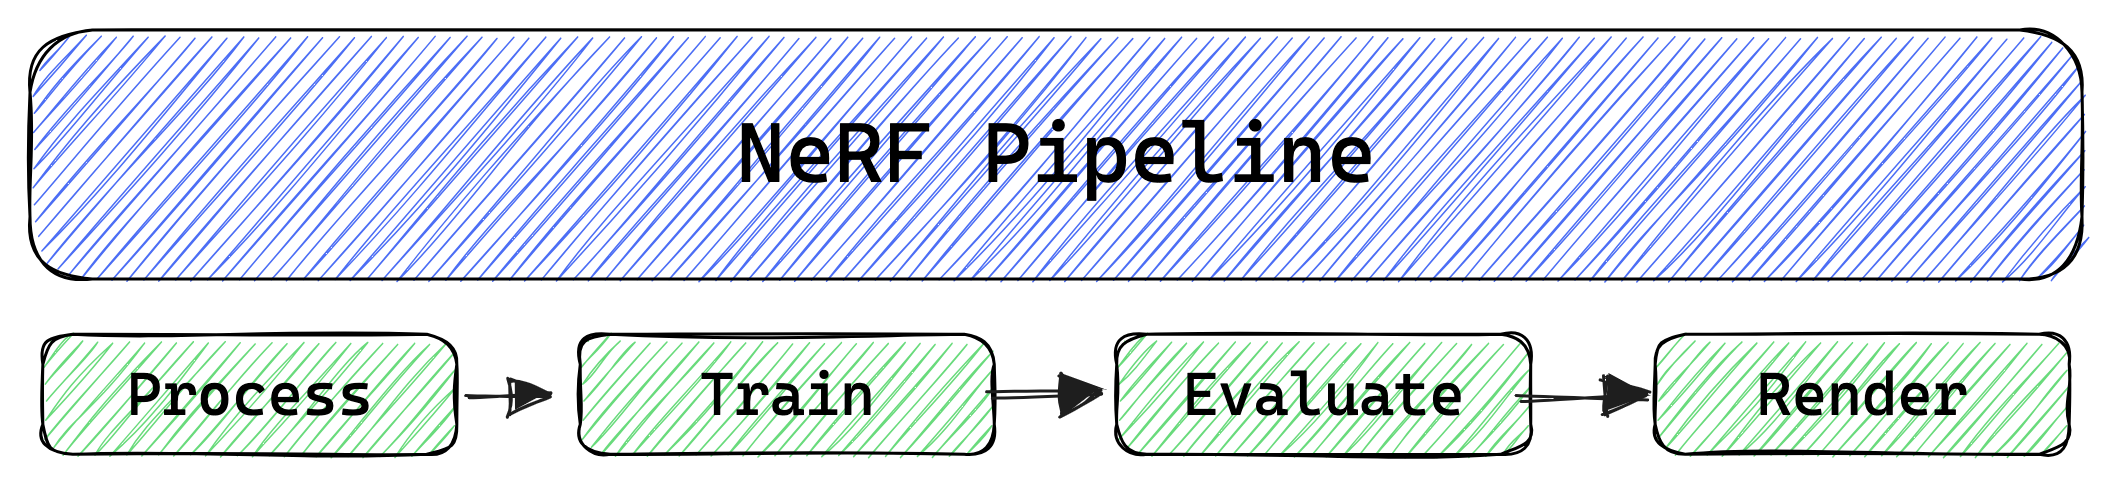
\includegraphics[width=1.0\textwidth]{figures/nerfstudio-pipeline.png}
    \caption{The components of the NeRF pipeline implemented in Nerfstudio.}
    \label{fig:nerfstudio-pipeline}
\end{figure}

The developed pipeline accepts a \texttt{Argument}-class used to configure the processing, training, evaluation, and rendering of the NerF. The most important parameters include:

\begin{itemize}
    \item \textbf{Input/output directory:} Defines where the data is located and where the output from the pipeline should be stored?
    \item \textbf{Model:} Defines which NeRF-model to use.
    \item \textbf{Settings for camera optimizer:} Defines if the NeRF should treat the camera poses as learnable parameters and optimize the camera poses.
    \item \textbf{Settings for side-by-side rendering:} Defines, among other things, which input-camera should be used as ground truth when rendering side-by-side.
\end{itemize}

\subsubsection{Process}

In most scenarios when working with real data, e.g. images of an object captured with a handheld camera, we don't have accurate camera poses. In those scenarios we have to pre-process the data in order to approximate camera poses for the captured images. It can be accomplished by leveraging SfM-algorithms as discussed in \autoref{sec:colmap}. In the scenario where the data is captured from CARLA, the poses are as accurate as they can be as they've been calculated in a deterministic environment. Assuming the CARLA-data is parsed according to the method discussed in \autoref{sec:carla-to-nerfstudio}, no further preprocessing is necessary.

\subsubsection{Train}
During training, the parameters in the model are optimized to represent the 3D scene. A batch of pixels is created for each training iteration. The default batch of 4096 pixels is obtained by randomly sampling the training images which defaults to $90\%$ of the total dataset, leaving $10\%$ as an evaluation dataset. Rays are marched through the sampled pixels and the model's networks predict RGB values and densities for the points sampled along the rays. The points' values are composited and the photometric loss, in combination with more complex losses, is computed. The losses are backpropagated through the model's networks and the ADAM optimizer\cite{adam} is used to update the network parameters.

For the Nerfacto-model, the primary model used throughout this thesis and previously discussed in \autoref{sec:nerfacto}, the training process entails backpropagating the loss and updating both the NeRF MLP and the proposal MLP. The Nerfacto-model leverages three different losses to guide the training; \textit{photometric loss}, \textit{interlevel loss}, and \textit{distortion loss}. \textit{Photometric loss} is the standard NeRF-loss explained in \autoref{eq:nerf-loss}. Interlevel- and distortion-loss are both from the Mip-NeRF 360\cite{barron_mip-nerf_2022} implementation explained in \autoref{sec:mipnerf360}. The interlevel loss encourages the model to generate consistent predictions across different levels of the multi-scale hierarchy, while the distortion loss encourages the model to generate smooth and continuous predictions.

Nerfstudio provides an API to configure all aspects of the pipeline, including dataset-split, number of pixels to sample, which optimizer to use, the configuration of the optimizer's exponential decay, the neural network's dimensionality, and much more. The implementation details and configurations used for the models in this thesis are attached in \autoref{sec:nerfstudio-train-parameters}.



\begin{comment}
The experiments in this thesis focus on the faster NeRF models implemented in Nerfstudio, namely Nerfacto (\autoref{sec:nerfacto}) and Instant NGP (\autoref{sec:instant-ngp}). Although the models are different, most of the shared model configurations are the same as can be seen in the model parameters included in \autoref{sec:nerfstudio-train-parameters}.

During training, the parameters in the model are trained to represent the 3D scene. For the Nerfacto-model, this entails backpropagating the error and updating both the NeRF MLP and the proposal MLP. The Nerfacto- and Instant NGP-model leverage 3 different losses to guide the training; \textit{RGB loss}, \textit{interlevel loss} and \textit{distortion loss}. \textit{RGB loss} is the standard NeRF-loss explained in \autoref{eq:nerf-loss}. Interlevel- and distortion-loss are both from the Mip-NeRF 360 implementation explained in \autoref{sec:mipnerf360}. The interlevel loss encourages the model to generate consistent predictions across different levels of the multi-scale hierarchy, while the distortion loss encourages the model to generate smooth and continuous predictions.

The training leverages the ADAM optimizer \cite{adam} for all networks within the model. The optimizer for the proposal networks and Nerfacto fields both use a learning rate of $1 \times 10^{-2}$, with no weight decay and $\epsilon=10^{-8}$, while the camera optimizer uses a learning rate of $6 \times 10^{-4}$, weight decay of $1 \times 10^{-2}$, and $\epsilon=10^{-8}$. All scenes were trained for 15,000 iterations, which is sufficient for achieving convergence. Training time for each scene is approximately 15-20 minutes when using an NVIDIA A100 GPU.

% TODO: Rewrite and reorganize. Write about how a batch of pixels are created for each training iteration
During the training of a NeRF, a batch of pixels is created for each training iteration. By default, this batch consists of 4096 pixels. To obtain these pixels, the training algorithm randomly samples them from all of the training images that are stored in RAM. However, this approach can be memory-intensive, especially when dealing with large datasets. To address this issue, the NeRF pipeline provides an option to set the parameter \texttt{–-pipeline.datamanager.train-num-images-to-sample-from}, which allows the user to sample pixels from a smaller subset of images. When using a smaller subset of images, the training algorithm will keep sampling from this subset unless the parameter \texttt{--num-times-to-repeat-images} is also set. This parameter specifies the number of training iterations after which the training algorithm should grab a new set of images to sample from. For instance, if \texttt{--num-times-to-repeat-images} is set to 1, the training algorithm will grab a new set of images to sample from every iteration. However, this approach can be computationally expensive and slow down the training process.
\end{comment}




\subsubsection{Evaluate}
To quantitatively evaluate the quality of the NeRF models, we utilize the metrics \acrshort{psnr}, \acrshort{ssim}, and \acrshort{lpips}, as elaborated upon in \autoref{sec:evaluating-nerfs}. During the evaluation, the camera poses from the evaluation dataset are fed into the trained model which subsequently renders the novel views. The rendered images are then compared against the corresponding ground truth images from the evaluation dataset according to the aforementioned metrics. 

The Nerfstudio API provides a script to load a model-checkpoint and compute these metrics, providing a quantitative assessment of the trained NeRF. To further facilitate the comparison of NeRF models across multiple experiments, an additional script was developed. This script load the evaluation outputs, compares the resulting metrics and produces a formatted LaTeX table that highlights the best and worst metrics.

%\begin{figure}[h]
    \centering
    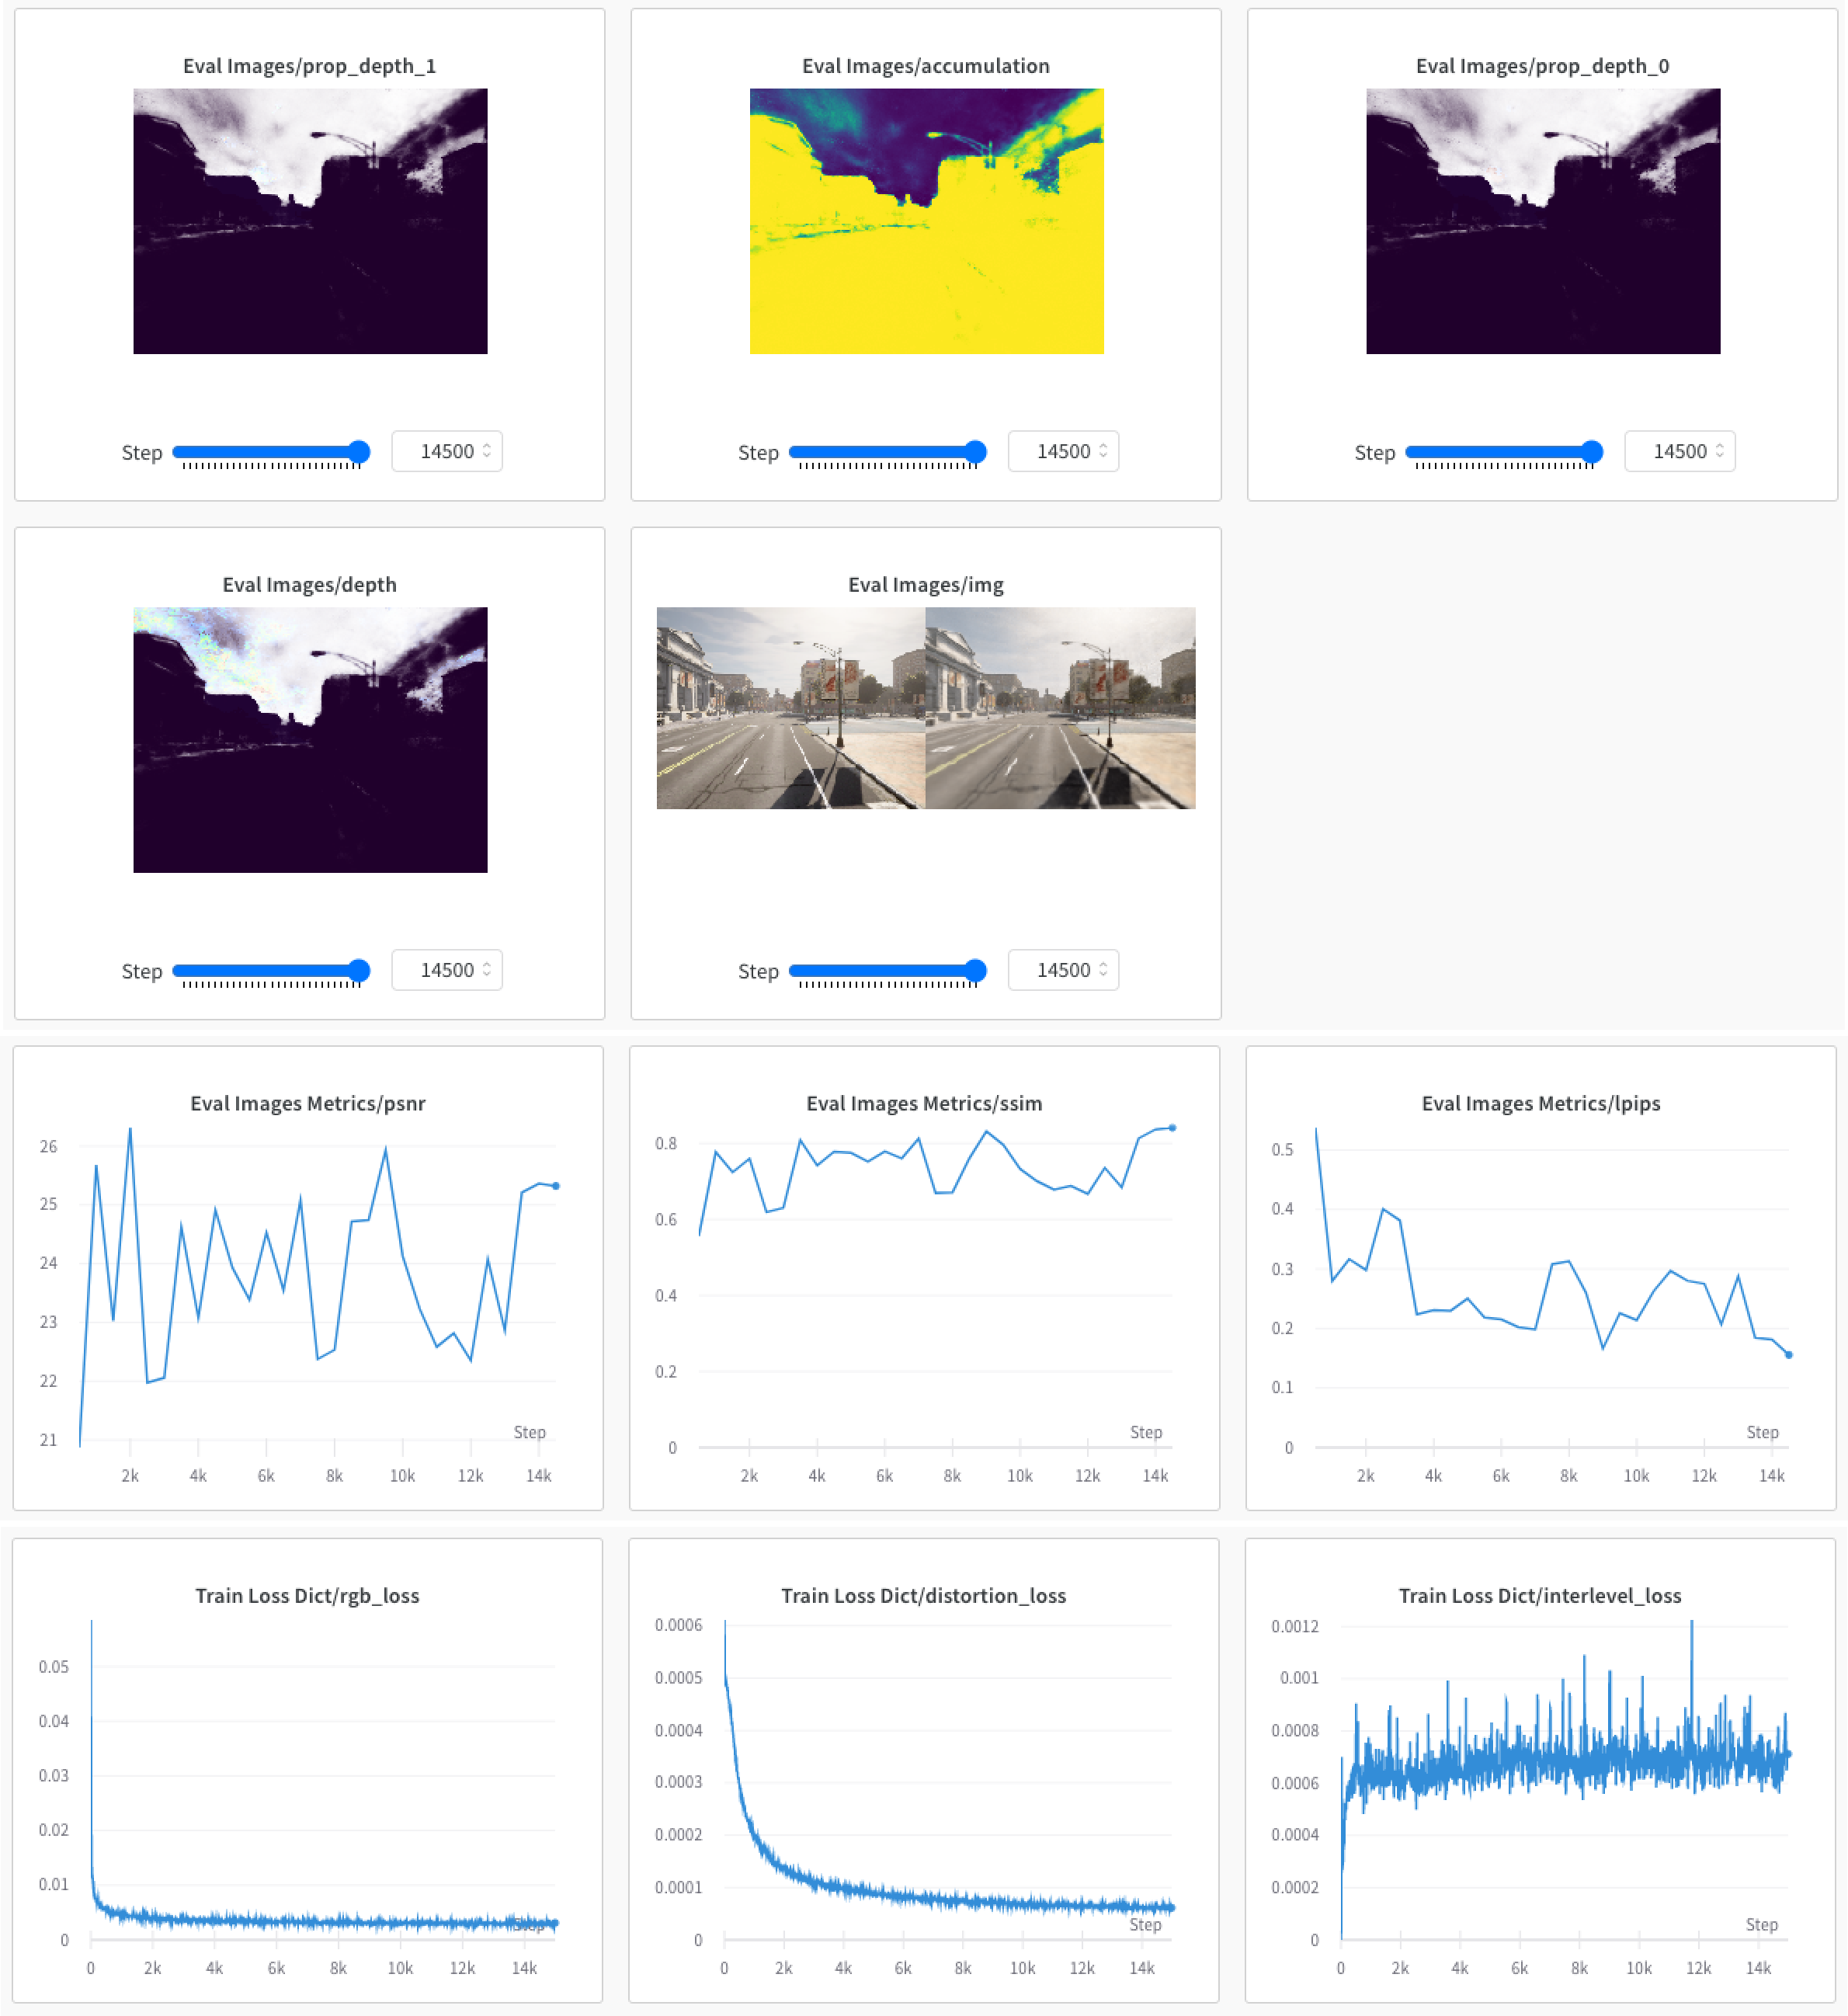
\includegraphics[width=1.0\textwidth]{figures/wandb-eval-data.png}
    \caption{Selection of evaluation data from Weights \& Biases \cite{wandb} for a NeRF training on a segment of synthetic data from CARLA.}
    \label{fig:wandb-eval-data}
\end{figure}

\subsubsection{Render}
%However, comparing experiments across different models and datasets with custom camera paths that will be slightly different for run/scene can be time-consuming and challenging. To address this issue, a script was developed to extract the ground truth camera path and use it in conjunction with the input images and trained NeRF model to create a side-by-side rendering. This approach has proven to be a useful means of qualitatively evaluating the performance of the NeRF models.

Although the quantitative metrics offer valuable insights into the quality of the model, it is crucial to assess the qualitative output. Consequently, all trained NeRF models are rendered in order to visually compare the results across different methods, configurations, and datasets.

The Nerfstudio API provides a script for rendering trained NeRF models given a camera path; a sequence of camera poses, each with a corresponding field of view and aspect ratio. The Nerfstudio viewer, depicted in \autoref{fig:nerfstudio-viewer-overview}, enables the creation and editing of camera paths, which can be exported and used for rendering. In addition to the possibility to create a custom camera path, a script to render the NeRF based on the input data's camera path was created. This option enables the creation of a side-by-side render, a useful and intuitive way to evaluate how well the NeRF has learned the input scene, i.e. qualitatively assessing the NeRF's performance.

\begin{figure}[H]
    \centering
    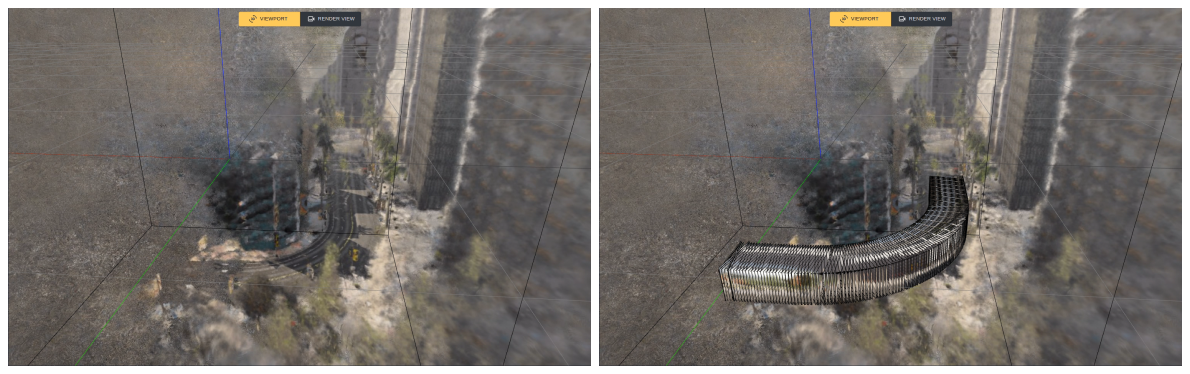
\includegraphics[width=1.0\textwidth]{figures/nerfstudio-viewer-overview.png}
    \caption{An overview of the Nerfstudio viewer. The scene seen on the left has been trained on the set of images and camera poses revealed in the image to the right.}
    \label{fig:nerfstudio-viewer-overview}
\end{figure}
%\begin{figure}[ht]
\centering
\begin{lstlisting}[language=json,linewidth=0.9\linewidth]
{
  "camera_type": "perspective",
  "render_height": 1080,
  "render_width": 1920,
  "fps": 24,
  "seconds": 10,
  "smoothness_value": 0.4624,
  "is_cycle": true,
  "camera_path": [
    {
      "camera_to_world": [
          0.0387,  0.0484,  0.9980,  0.4483,
          0.9992, -0.0018, -0.0386,  0.9853,
         -2.0166,  0.9988, -0.0485, -0.0018,
          0,       0,       0,       1
      ],
      "fov": 90,
      "aspect": 1.6678200692041523
    },
    ...
  ],
  "keyframes": [...],
}

\end{lstlisting}
\caption{Example of a \textit{camera-path.json}-file used to render a specific path for a trained NeRF in the Nerfstudio API.}
\label{code:camera-path-example}
\end{figure}




\begin{comment}
% TODO: If I'm to use this, I have to double check if it's correct
\begin{equation} \label{eq:distortion_loss}
\mathcal{L}_{\text{distortion}} = \frac{1}{N} \sum_{i=1}^{N} \left(\sum_{j=1}^{M_i} w_{ij} \sum_{k=1}^{M_i} w_{ik} \left| \frac{t_{ij} + t_{ik}}{2} - \frac{t_{i,j-1} + t_{i,k-1}}{2} \right| \right) + \frac{1}{3N} \sum_{i=1}^{N} \sum_{j=1}^{M_i} w_{ij}^2 (t_{ij} - t_{i,j-1})
\end{equation}

\begin{center}
    \small{where $N$ is the number of ray samples, $M_i$ is the number of samples for the $i$-th ray, $w_{ij}$ is the weight for the $j$-th sample of the $i$-th ray, $t_{ij}$ is the $j$-th sample of the $i$-th ray in the $s$-domain, and $t_{i,j-1}$ is the $(j-1)$-th sample of the $i$-th ray in the $s$-domain.}
\end{center}


\begin{equation} \label{eq:interlevel_loss}
\mathcal{L}_{\text{interlevel}} = \frac{1}{N} \sum_{i=1}^{N-1} \frac{1}{M_i} \sum_{j=1}^{M_i} \left(\max(0, w_j - w_{\text{outer},ij})\right)^2 \cdot \frac{1}{w_j + \epsilon}
\end{equation}

\begin{center}
    \small{where $N$ is the number of ray samples, $M_i$ is the number of samples for the $i$-th ray, $w_j$ is the weight for the $j$-th sample of the $i$-th ray, $w_{\text{outer},ij}$ is the upper bound of the inner histogram for the $j$-th sample of the $i$-th ray, and $\epsilon$ is a small constant.}
\end{center}
\end{comment}




%\section{Establish a CARLA-baseline}
\section{Establishing the CARLA-Baseline}
\begin{comment}
Premise: Have a pipeline to test multiple CARLA-setups
Question: How do I find a CARLA-baseline?

\begin{itemize}
    \item Why do I need a baseline?
    \item How do I find suitable experiments?
    \item How do I evaluate the experiments against each other?
\end{itemize}
\end{comment}

A pipeline to evaluate numerous CARLA configurations to identify a configuration that generates high-quality data for NeRF training has been established. In order to facilitate further experiments, a baseline need to be created.

The experiments chosen to define a suitable baseline are mostly based on heuristics and knowledge of what's important for good NeRF results. When capturing video or images for a NeRF it’s important that the scene is well-lit, that the captured images aren't blurry, and that there are no transient objects present. If the camera poses of the captured images are to be approximated with the use of SfM-methods like COLMAP, it's also very important that the images have an overlap in order to secure feature-matching across the images. The five experiments chosen to define the baseline, which will be elaborated upon in \autoref{sec:experiments-and-results}, were:

\begin{itemize}
    \item \textbf{Camera setup:} How many cameras should be mounted to the ego vehicle, and in what translation and rotation?
    \item \textbf{Capacity:} How long should the segments used to capture data be?
    \item \textbf{Number of frames:} How many frames to capture?
    \item \textbf{Image size:} What resolution should the mounted cameras capture at?
    \item \textbf{Vehicle speed:} At what speed should the ego vehicle drive while capturing data?
\end{itemize}

The best results from each of the experiments, based on qualitative results and quantitative metrics discussed in \autoref{sec:evaluating-nerfs}, were used to iteratively build a baseline used for further experiments.
















%\section{Use the CARLA-baseline}
\section{Comparative Experiments with the CARLA-Baseline}
\begin{comment}
Premise: Have a CARLA-baseline for further experiments
Question: Which further experiments should I conduct?

\begin{itemize}
    \item Find the efficiency of pose refinement
\end{itemize}
\end{comment}

With a defined baseline, we can now evaluate the impact of different NeRF- and capture settings on the quality of the resulting models. This provides a starting point for conducting further experiments, which can be systematically varied to explore the factors that impact the quality of resulting trained NeRF. Additionally, we can simulate real-world capture scenarios using the synthetic data generated by the baseline. The specific experiments ran with the baseline, elaborated upon in \autoref{sec:experiments-and-results}, were:

\begin{itemize}
    \item \textbf{Noisy sensor readings:} Noise in the camera pose due to inaccurate readings from the GPS/GNSS.
    \item \textbf{Approximated poses vs. perfect poses:} How effective is COLMAP in approximating the camera poses, as opposed to the perfect camera poses extracted from CARLA?
    \item \textbf{Different models:} How do the different NeRF models perform against each other?
    \item \textbf{Improve capacity - Block-NeRF PoC}: How can we train NeRFs on increasingly larger scenes?
\end{itemize}




















































%\section{Extend the CARLA-baseline to support large scale scenes} \label{sec:method-block-nerf}
\section{Extending the Pipeline to Support Large-Scale Scenes} \label{sec:method-block-nerf}

\begin{comment}
Premise: Have found the CARLA-baseline to work well on shorter segments. As discussed multiple papers, the capacity is limited.
Premise \#2: Since I operate in a synthetic environment, I have perfect poses which simplifies the process.
Question: How do I implement Block-NeRF in Nerfstudio, given perfect poses?

\begin{itemize}
    \item Split the dataset into multiple datasets
    \item Train each seperately
    \item Create a camera path
    \item Render the camera path for each NeRF
\end{itemize}
\end{comment}

The NeRF model in the defined baseline has proven to perform well. When we change the route of the CARLA-baseline and create a larger dataset, spanning kilometers of road data, the NeRF models evidently have a hard time generating high-quality image synthesis. That result is expected as the models' underlying MLPs only have a certain capacity. We could increase the capacity by increasing the number of hidden layers and neurons per layer, but this would lead to linearly increasing training -and rendering times. Rendering is already an expensive operation which further supports the claim for another solution.

As discussed in \autoref{sec:block-nerf} it is an open research field within the NeRF community to expand the capability of NeRFs to enable the representation of large scenes. Compared to the other fields covered in NeRF research, there aren't a lot of papers exploring large-scale NeRFs, which might be due to the amount of data needed and the corresponding data capture endeavor. Luckily, we have constructed a pipeline that automates synthetic data capture and the subsequent processing, training, evaluation and rendering of the NeRF. Due to this we expand the pipeline to enable the evaluation of a large-scale NeRF approach, based on a naive implementation of Block-NeRf \cite{tancik_block-nerf_2022}.

% Explain the naive Block-NeRF implementation
One of the main challenges in implementing Block-NeRF is obtaining the camera poses for the captured images. Traditional SfM methods, such as COLMAP, become computationally expensive and slow when dealing with large datasets, as is demonstrated by the feature matching complexity overview presented in Table \ref{tab:colmap-feature-complexity}. However, being in possession of the image's corresponding camera poses simplifies the process. Assuming we have both, the steps for creating a Block-NeRF model can be summarized as follows:

\begin{itemize}
    \item \textbf{Split the dataset into multiple smaller datasets:} 

    The \textit{split\_transforms} function takes an original \texttt{transforms.json} file and a sequence of images and splits them into $n$ roughly equal-sized new datasets, which are formatted according to the structure shown in \autoref{fig:nerfstudio-file-structure}, resulting in a file structure shown in \autoref{fig:block-nerf-file-structure}.

    \item \textbf{Train separate NeRFs on the split dataset:} 

    Run a standard training loop on each of the $n$ datasets created in the previous step.
    
    \item \textbf{Create a camera path spanning the segments contained in the complete dataset:}
    
    There are multiple options for creating the camera path: The camera path can be created in the Nerfstudio viewer, a previously exported camera path can be used, or a helper function could be utilized to leverage the camera path of the input images which will later also be used to generate the side-by-side render. No matter which option is chosen, an important aspect in this naive implementation is that the camera-to-world matrices in the camera path are in the same scale and coordinate system as the Block-NeRF's \texttt{transforms.json}-files.
    
    \item \textbf{Create a lookup table for which Block to render which camera pose:}

    In order to know which NeRF to render given a specific 3D point and direction, expressed by the $4x4$ camera-to-world matrix in the camera path, we create a naive lookup table. The lookup table is indexed on the camera path's location index and returns the Block-NeRF with the minimum Euclidean distance.

    \item \textbf{Modify the camera path to account for the offset, transformations, and scales of each NeRF:}
    
    Before a NeRF is trained, the input camera poses are scaled to fit a $[-1, 1]$ bounding box, and transformed so that the average up vector is aligned with the Z-axis. The respective transformation which is carried out to make the training easier is stored in a \texttt{dataparser\_transforms.json}-file containing the applied transform matrix and scale. Each of the Block-NeRF's \texttt{dataparser\_transforms.json}-file is different, and in order to render the desired camera path seamlessly across the different NeRFs according to the lookup table, we have to augment it to account for the transformations. We achieve this by creating a new, transformed camera path where the segments which are to be rendered by $\text{Block-NeRF}_i$ have their camera-to-world transformed by applying $\text{Block-NeRF}_i$'s scale $s$ and transformation matrix $t$. 
    
    \item \textbf{Render the created camera path:}

    Building upon Nerfstudio's render script, the lookup table is passed as a parameter and used to conditionally choose which model to render. As all the changes to the camera path have been done a priori, the resulting render is a seamless video through the scene leveraging multiple Block-NeRFs.
\end{itemize}



\begin{comment}
\begin{algorithmic}[1]
\Function{transform\_to\_single\_camera\_path}{}
    \State $block\_lookup$ \Comment{Lookup block to render at a certain c2w}
    \For{$c2w$ \textbf{in} $camera\_path$}
        \State $block \gets block\_lookup[c2w]$
        \State $t \gets block.dataparser\_transform["transform"]$
        \State $s \gets block.dataparser\_transform["scale"]$
        \State $new\_c2w \gets (t \times c2w) \times s$
        \State $camera \gets new\_c2w$
    \EndFor
\EndFunction
\end{algorithmic}


% TODO: If I'm to use this algorithm I have to go over it and fix it.
\begin{algorithmic}[1]
\Function{transform\_to\_single\_camera\_path}{$camera\_path\_path, block\_lookup, dataparser\_transform\_paths, export\_dir$}
    \State $original\_camera\_path \gets$ \Call{load\_json}{$camera\_path\_path$}
    \State $new\_camera\_path \gets$ \Call{copy.deepcopy}{$original\_camera\_path$}

    \For{$i \gets 0$ \textbf{to} $len(new\_camera\_path["camera\_path"]) - 1$}
        \State $block\_name \gets block\_lookup[str(i)]$
        \State $transform \gets$ \Call{load\_json}{$dataparser\_transform\_paths[block\_name]$}
        \State $t \gets$ \Call{np.array}{$transform["transform"]$}
        \State $s \gets transform["scale"]$

        \State $c2w \gets$ \Call{np.array}{$new\_camera\_path["camera\_path"][i]["camera\_to\_world"]$}.\Call{reshape}{4, 4}
        \State $c2w \gets (t \times c2w) \times s$
        \State $c2w \gets$ \Call{np.vstack}{($c2w$, \Call{np.array}{[0, 0, 0, 1]})}
        \State $new\_camera\_path["camera\_path"][i]["camera\_to\_world"] \gets c2w.\Call{reshape}{16}.\Call{tolist}{}$
    \EndFor
\EndFunction
\end{algorithmic}
\end{comment}

\begin{figure}[ht]
\centering
\begin{forest}
for tree={
      parent anchor=south west,
      child anchor=west,
      anchor=mid west,
      inner ysep=1pt,
      grow'=0,
      align=left,
      edge path={
        \noexpand\path [draw, \forestoption{edge}] (!u.parent anchor) ++(1em,0) |- (.child anchor)\forestoption{edge label};
      },
      font=\sffamily,
      if n children=0{}{
        delay={
          prepend={[,phantom, calign with current]}
        }
      },
      fit=band,
      before computing xy={
        l=2em
      }
    }
[block\_nerf\/
[ block\_0\/
  [ images/
    [ 0001.png ]
    [ 0002.png ]
    [ 0003.png ]
    [ \ldots{} ]
  ]
  [ transforms.json ]
]
[\ldots{}]
[ block\_n\/
  [ \ldots{} ]
]
]
\end{forest}
\caption[Block-NeRF file structure]{Block-NeRF file structure after having split a single dataset into multiple smaller datasets.}
\label{fig:block-nerf-file-structure}
\end{figure}

%A large part of what is tricky with implementing Block-NeRF is obtaining the captured images' camera poses. COLMAP becomes painfully slow with large datasets, as can be seen by the feature matching complexity overview in \autoref{tab:colmap-feature-complexity}. When you capture the images' corresponding camera pose simultaneously as you capture the image, it's another story. With both the images and camera poses, the main steps in creating the Block-NeRF are 1) splitting the dataset into multiple smaller datasets, 2) training separate NeRFs on the split datasets, 3) creating a camera path and modifying it to take into account the offset between each NeRF, 4) and lastly rendering the camera path by combining renders from suitable NeRFs.














%\section{Extending the pipeline to enable input of real data} \label{sec:extending-real-data}
\section{Extending the Pipeline to Support Real Data} \label{sec:extending-real-data}

\begin{comment}
Premise: Have a working pipeline to collect, train and render novel views from CARLA
Question: How can this pipeline be extended to enable input of real data?

\begin{itemize}
    \item How to collect images and camera poses from the car?
    \item Which changes had to be done to the pipeline to support this change?
\end{itemize}
\end{comment}

%\begin{figure}[!h]
    \centering
    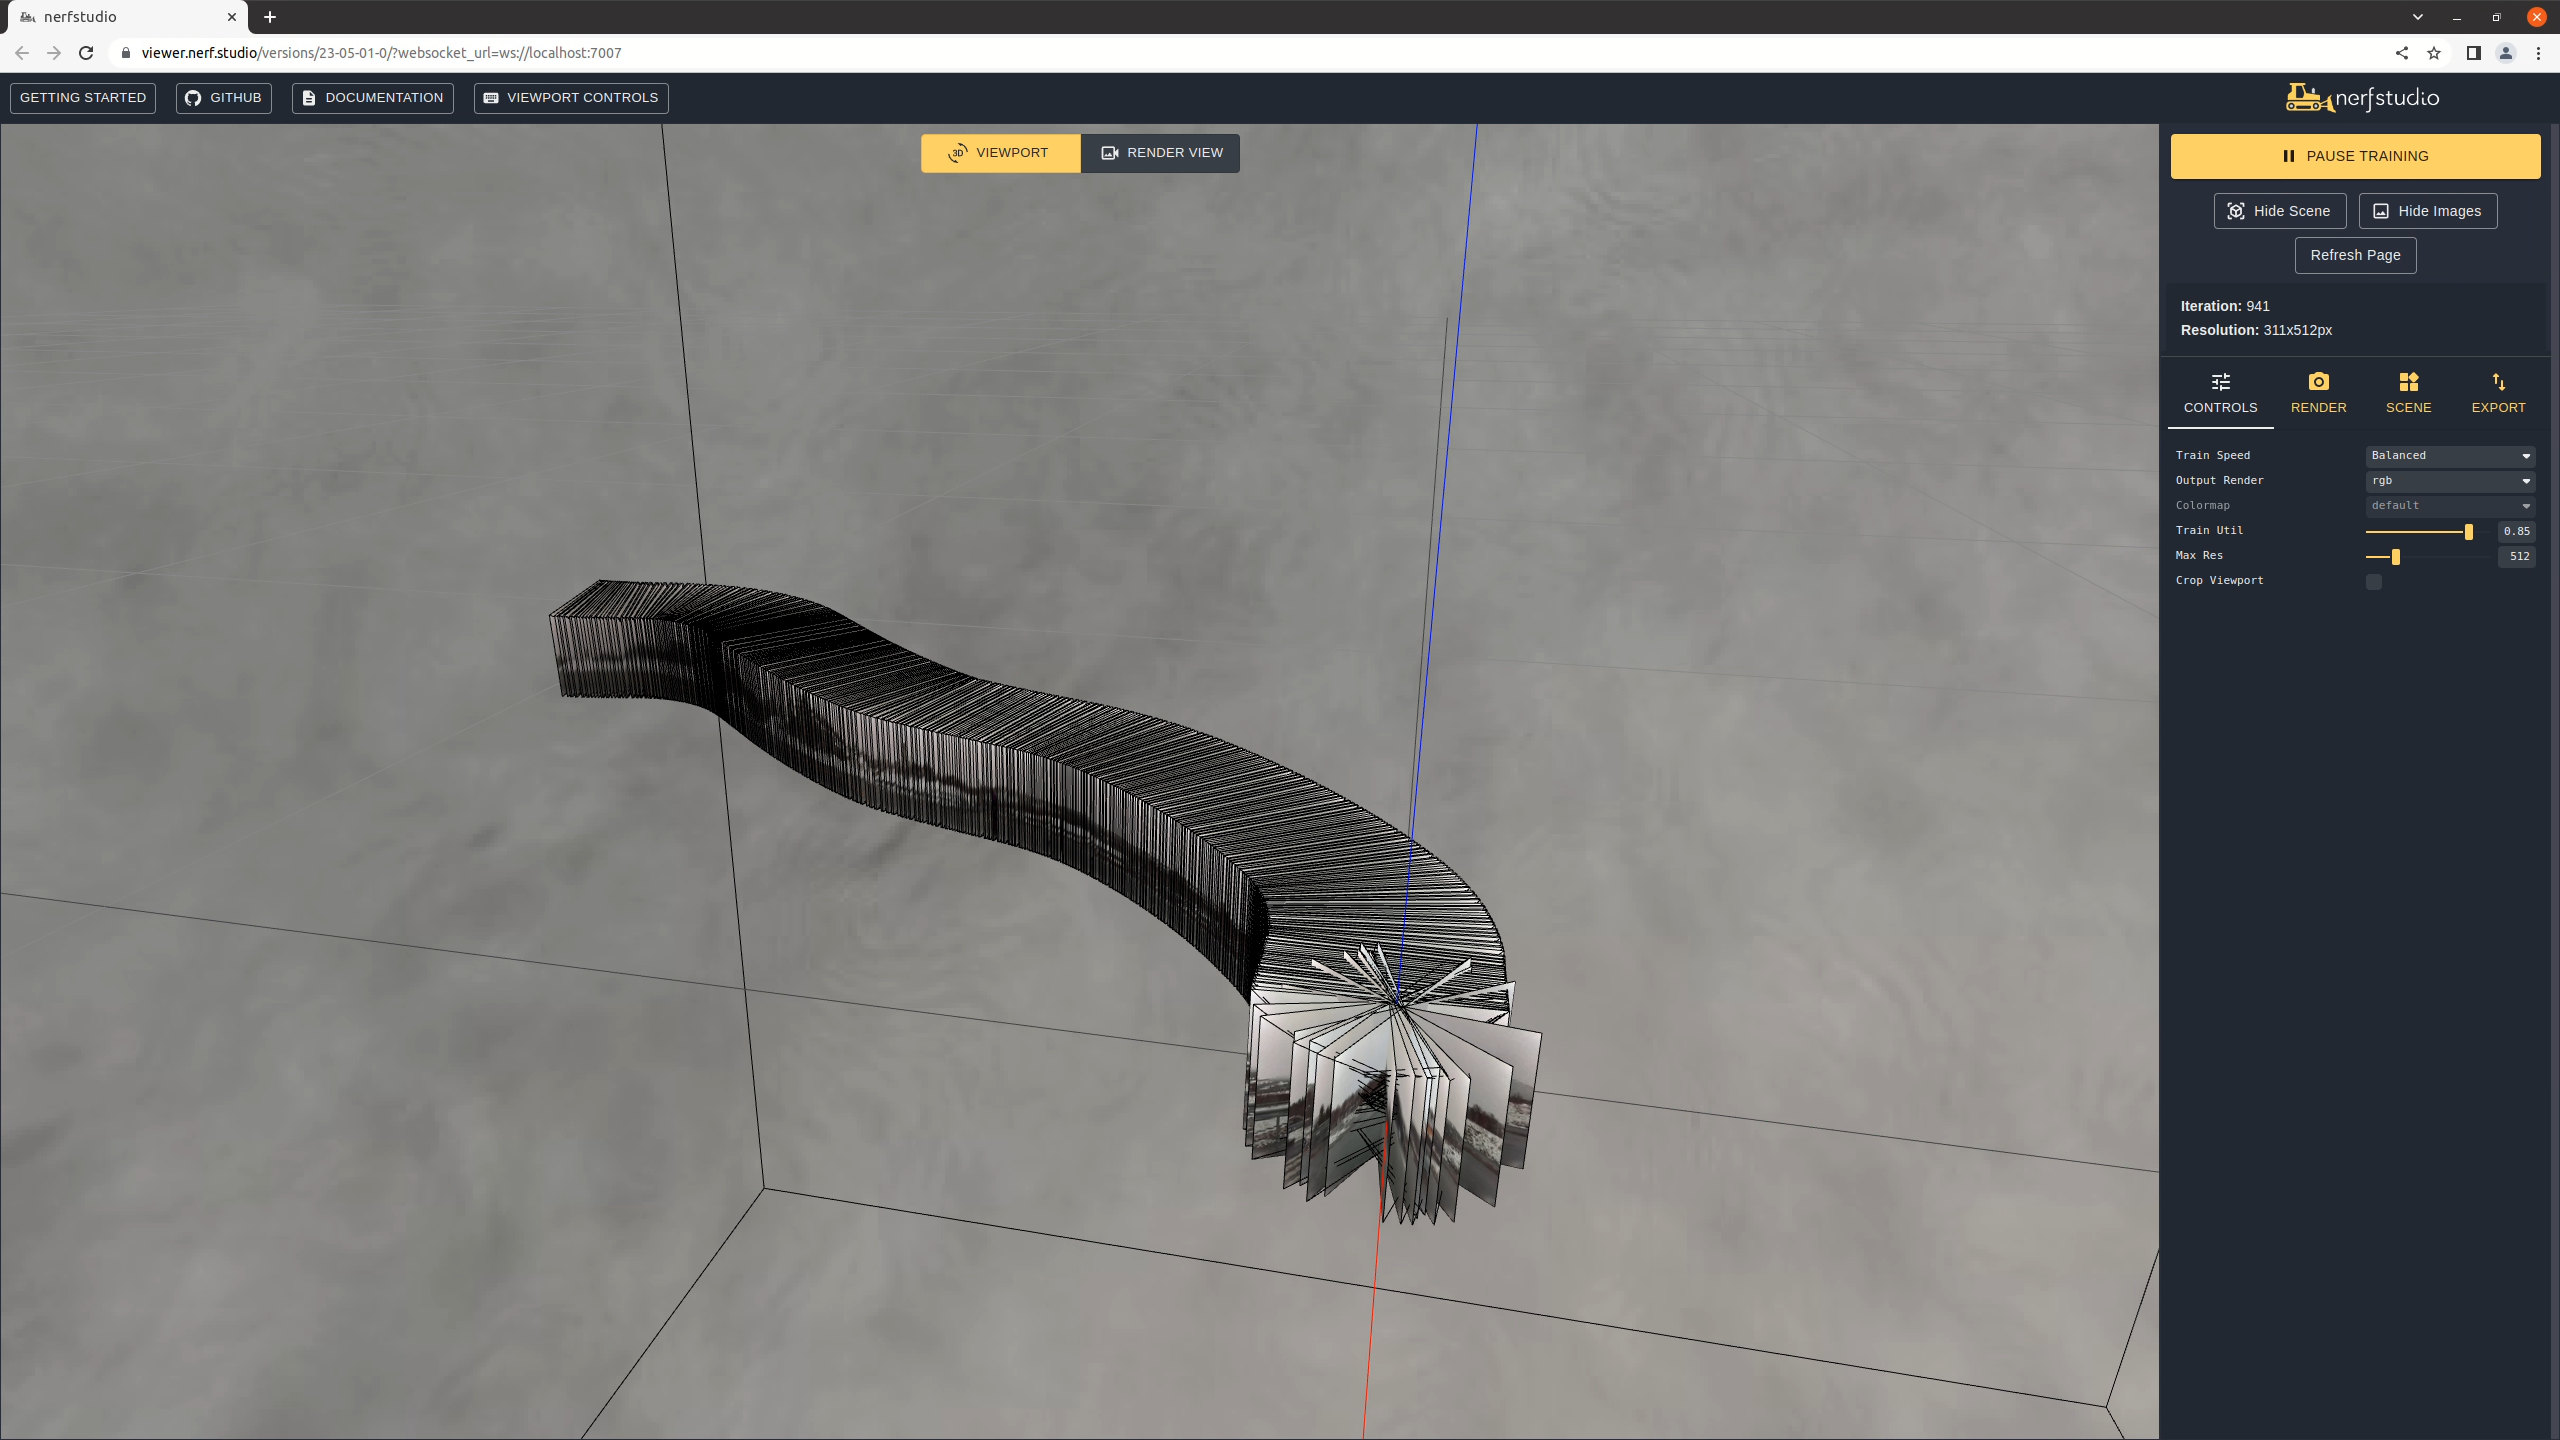
\includegraphics[width=1.0\textwidth]{figures/nerfstudio_real_data_estimated_poses.png}
    \caption{Real data with estimated poses viewed in the Nerfstudio Viewer}
    \label{fig:nerfstudio_real_data_estimated_poses}
\end{figure}

\begin{comment}
Introduction
- Making NeRFs with real data is the usual way to go about generating NeRFs.
- The challenge is in capturing this data from cameras mounted on vehicles, in uncontrolled environment.

How do I expand the pipeline?
- How is the data captured? Introduce the NAPLab-car, the sensors, etc.
- How do I read this data? Mention the Aksel and Mathias' repository.
    - Use FFMPEG to read the .h264-video and serve the frames with a generator-function.
    - Use regex to parse a file with GPS data formatted as NMEA (National Marine Electronics Association) sentences, a standard messages used by GPS (Global Positioning System) receivers to communicate with other devices, such as computers or chartplotters. Each GPS-datapoint is seved with a generator-function the same way as with the video-frames.
    - The camera is synchronized to the closest frame in time to the GPS timestamp using custom code. "- Custom code is used to synchronize the camera to the frame closest in time with the GPS timestamp."
    - After synchronization, I can loop through the synchronized sensor data with a regular loop.
- Premise: Have synchronized image- and GPS-data.
- Create a NAPLabDataParser that implements the same methods as the CarlaDataParser. The main difference is in the implementation of the transform-function. 
- The transformation matrix is created by :
    - Store the initial GPS lat, long and alt, and use it as the reference point.
    - The reference point is utilized in order to convert latitude, longitude, altitude of subsequent GPS-readings to North, East, Down from the observer, i.e. the reference point.
    - NED is then converted to ENU and then to blender coordinate conventions.
    - The rotation is estimated with trigonometry by comparing subsequent GPS-readings.
    - The translation and rotation is combined into a transformation matrix.
- The intrinsics are computed in the same way as discussed in \autoref{sec:carla-to-nerfstudio}.
- The transformation matrix and intrinsics are combined into a transform.json
- The exported transform.json and images are in the same format as the output from the CarlaDataParser, so the following pipeline remains unchanged.
\end{comment}

The pipeline from data capture in CARLA to image synthesis with a trained NeRF has demonstrated efficacy. This final section of the method-chapter discusses how the pipeline is extended to enable the input of real data, not captured in a virtual environment like the CARLA simulator.

The traditional approach for generating NeRFs involves the use of real data. The real data is usually captured from handheld cameras. With handheld cameras it is uncomplicated to capture well-lit, non-blurry, object-centric images that doesn't contain transient objects. Until now we've used a virtual environment to capture data as it provides a fully controllable environment in which we can test different setups and ensure optimal conditions. The following challenge in this project is capturing high-quality data from sensors, mounted to a moving vehicle, that is suitable for training NeRF models.

To capture data, we utilized the\acrshort{naplab} car \cite{naplab}. The NAPLab car is fitted with multiple sensors, including cameras, \acrshort{gps}/\acrshort{gnss}, and \acrshort{lidar}. The cameras capture data with a resolution of $1920 \times 1080$. The GPS/GNSS-system consists of two Swift Navigation Duro Ruggedized Receivers \cite{swift_navigation_duro_manual}, which offer superior positioning accuracy compared to regular GPS/GNSS systems. According to the manufacturer’s documentation, each Duro module has a horizontal position accuracy of 0.75 meters (\acrlong{cep} [\acrshort{cep}] of 50 in \acrlong{sbas} [\acrshort{sbas}] mode) without \acrfull{rtk}, and can achieve centimeter-level accuracy with \acrshort{rtk} enabled. This high level of accuracy enables the capture of rough camera poses alongside the images.

After having captured data with the NAPLab car, the data has to be parsed and processed before it can be transformed into the expected Nerfstudio-format. A repository\footnote{\url{https://github.com/aasewold/experiments/}} that streamlines the reading and parsing of NAPLab's data into a manageable format was leveraged. In order to read the video data, FFMPEG is utilized to transform .h264-files into sequences of \texttt{np.ndarray}s that are subsequently served by a generator function. The GPS data is formatted as \acrfull{nmea} sentences, a message standard used by GPS receivers to communicate with other devices. This GPS data is read and parsed using regex and subsequently served by a generator function. 

A key aspect of the data parsing is the synchronization of the camera with the GPS timestamp. This is achieved by leveraging functionality from the same repository that aligns the camera with the frame closest in time to the GPS timestamp. Following synchronization, the sensor data can be accessed and further processed using a regular loop.

The synchronized data have to be converted into Nerfstudio's data format in order to be used in the predefined pipeline. In order to achieve this, a \texttt{NAPLabDataParser} that implements the same methods as the \texttt{CarlaDataParser}, is created. The primary difference is the implementation of the transformation function that converts the translation and rotation data from one coordinate convention to another. The transformation matrix construction process involves several steps:

\begin{itemize}
    \item The initial GPS latitude, longitude, and altitude readings are stored as the reference point.
    \item The \texttt{geodetic2ned} function from the \texttt{pymap3d} library \cite{Hirsch_PyGemini} is used to transform GPS data into \acrfull{ned} coordinates.
    \item The NED coordinates are then converted to \acrfull{enu} coordinates and then to Blender coordinate conventions.
    \item The cameras' rotation is estimated by comparing adjacent GPS data points using trigonometry.
    \item The resulting translation and rotation data are combined into a single transformation matrix.
\end{itemize}

The computation of intrinsic values follows the same methodology as discussed in \autoref{sec:carla-to-nerfstudio}. These intrinsics, in combination with the transformation matrix, are assembled into a \texttt{transforms.json} file. The output from the \texttt{NAPLabDataParser}, i.e., the \texttt{transforms.json} file and images, is in the same format as that from the \texttt{CarlaDataParser}. Therefore, the subsequent stages of the pipeline remain unaffected, ensuring the smooth extension from synthetic to real data inputs.

The dataset captured from the NAPLab car is presented in \autoref{fig:naplab-dataset}.

\begin{figure}[h]
    \centering
    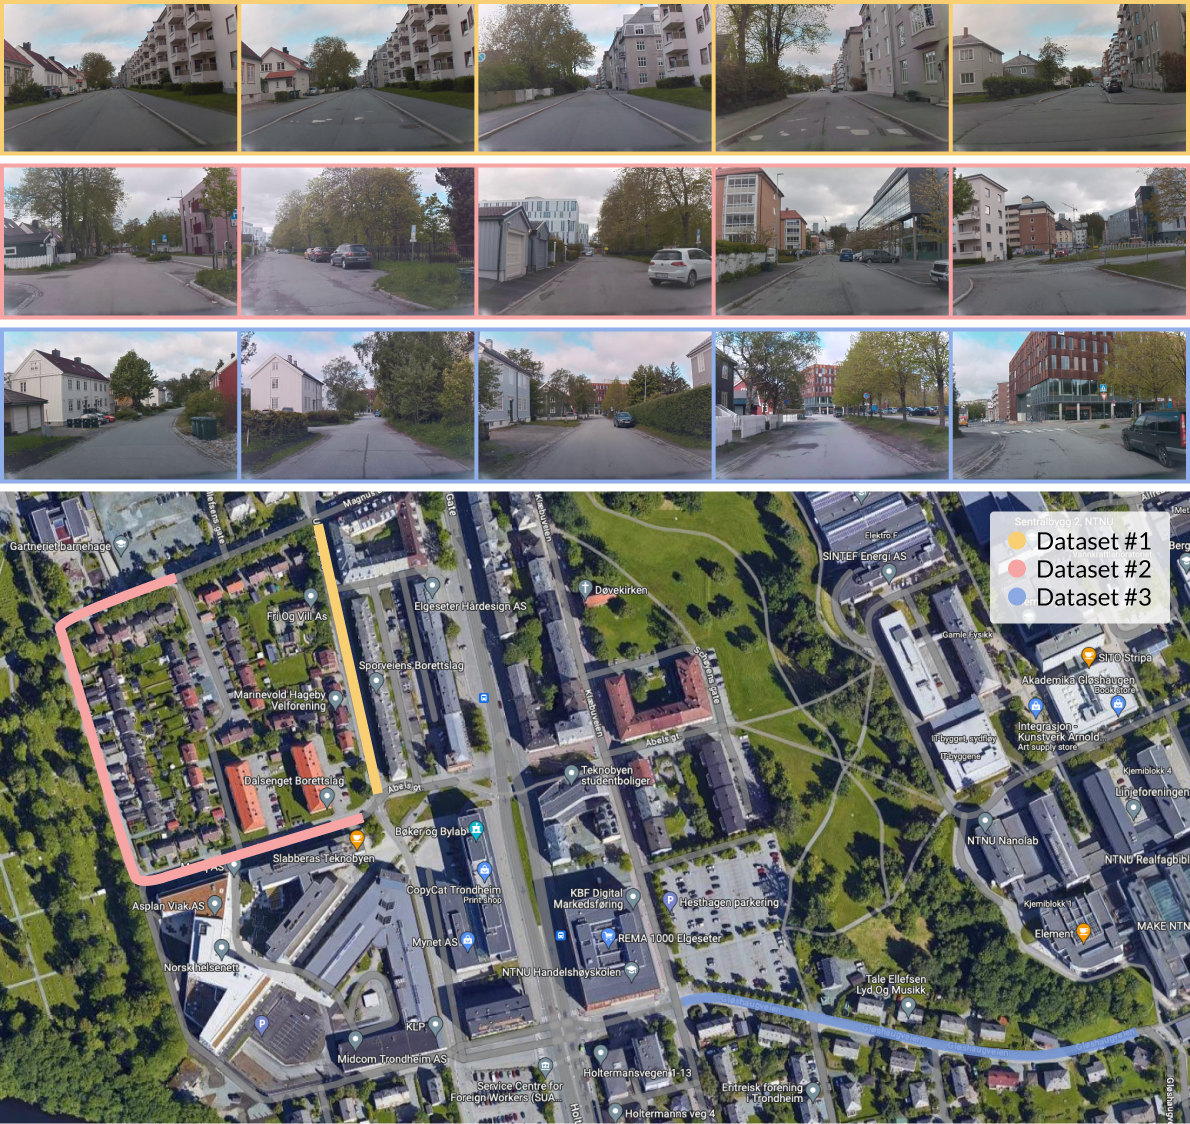
\includegraphics[width=1.0\textwidth]{figures/naplab-dataset.png}
    \caption[The datasets captured from the NAPLab car.]{Overview of the datasets of real data captured from the NAPLab car. 1) contains 235 images over a straight road segment of approximately 170m, 2) contains 199 images over a segment of approximately 380m, 3) contains 160 images over a segment of approximately 280m.}
    \label{fig:naplab-dataset}
\end{figure}





\begin{comment}
The traditional approach for generating Neural Radiance Fields (NeRFs) involves the use of real data. However, collecting this real data presents a unique challenge when dealing with cameras mounted on vehicles operating in uncontrolled environments. Overcoming this obstacle requires an innovative expansion of the existing data processing pipeline.

Data capture is achieved with the assistance of a specially outfitted vehicle, known as the NAPLab-car, equipped with an array of sensors for comprehensive environmental data collection. Subsequently, the captured data is read and processed using the repository developed by Aksel and Mathias.

This repository utilizes FFMPEG software to read the .h264-video, serving the video frames through a generator function. In parallel, a regular expression (regex) is used to parse GPS data structured as NMEA (National Marine Electronics Association) sentences - standard messages exchanged between GPS receivers and auxiliary devices like computers or chartplotters. Each parsed GPS datapoint is then served via a generator function akin to the video frames.

A key aspect of the pipeline expansion is the synchronization of the camera with the GPS timestamp. This is achieved with custom code that aligns the camera with the frame closest in time to the GPS timestamp. Following synchronization, the sensor data can be accessed and navigated using a regular loop.

Building on this premise of synchronized image and GPS data, a NAPLabDataParser is created to mimic the functionality of the CarlaDataParser. The primary distinction lies in the implementation of the transform function. The transformation matrix construction process involves several steps:

- The initial GPS latitude, longitude, and altitude readings are stored and utilized as a reference point.
- This reference point serves as a basis to convert subsequent GPS readings into North, East, Down (NED) coordinates relative to the observer.
- NED coordinates are subsequently converted to East, North, Up (ENU) and further to Blender coordinate conventions.
- Subsequent GPS readings are compared to estimate rotation using trigonometry.
- Finally, the translation and rotation data are integrated into a single transformation matrix.

The computation of intrinsic values follows the same methodology as discussed in \autoref{sec:carla-to-nerfstudio}. These intrinsics, in combination with the transformation matrix, are assembled into a transforms.json file.

The output from the NAPLabDataParser, i.e., the transforms.json file and images, is analogous in format to that from the CarlaDataParser. Therefore, the subsequent stages of the pipeline remain unaffected, ensuring the smooth transition from synthetic to real data inputs.
\end{comment}
\chapter{Results}

This chapter presents the results of multiple experiments conducted on the datasets described in \autoref{sec:dataset}. The aim is to showcase some findings and give insight into the process of utilizing NeRFs. The results are both quantitative, measured by the metrics discussed in \autoref{sec:evaluating-nerfs}, and qualitative. The qualitative results are hard to visualize in this report because the only option would be to attach frames from the resulting render. Although this yields an indication of the resulting rendering's quality, a rendered video exposes greater details in terms of correspondences between frames, potential artifacts, and learned geometry. In order to showcase these results, there's a companion page found \href{https://absorbing-peace-5f6.notion.site/NeRF-Renders-1260636ed8e44f8e8e4d45bd9fc6dda4#1edb5c8c9f86444db1902a18243b6e51}{here} where different renders can be browsed and compared.

\vspace{2mm} %5mm vertical space
\noindent \textbf{\href{https://absorbing-peace-5f6.notion.site/NeRF-Renders-1260636ed8e44f8e8e4d45bd9fc6dda4\#1edb5c8c9f86444db1902a18243b6e51}{Link to companion page with video renders}}

\begin{comment}

Experiments:
- Explore the impact of capturing
    - Capturing NeRFs in different ways
        - Walking, standing still, sparsely, densely, linearly, around an object
    - Capturing video, images, polycam
        - Better/worse quality with polycam or COLMAP
    - Capturing different kind of scenes
        - Bounded/Unbounded 
    - Capturing in different conditions
    - Capturing 
    
- Explore the impact of dataset size
    - Extract different amounts of images from the video ✅
        - Simulate driving by walking up and back a street multiple times ✅
    - How much data is required until COLMAP becomes a bottleneck

- Explore the impact of area-size
    - Remember to point out that area is poorly defined since scale is perspective relative, depending on the level of detail you want. ✅
    - Area must be defined for a certain scene type. E.g. street view, aerial view, unbounded in multiple directions, bounded in all directions

- Explore the impact of different methods
    - instant-npg, nerfacto, NeRF

Metrics
- Quantitative
    - PSNR, LPIPS, SSIM
- Qualitative
    - Compare images side-by-side



Research questions:
- To what extent does a good capture impact the result of a NeRF
- How much data is required until COLMAP becomes a bottleneck?
- What is the capacity of a NeRF when optimizing a street view scene?

SCENES:
- Bounded scene
- Unbounded scene
- Walking
- Standing still
- Street-view
\end{comment}



\section{Different methods}
There are multiple different methods proposed for reconstructing 3D scenes and rendering novel views. In this experiment we compare four of the methods that are currently implemented in Nerfstudio. Even though the original NeRF-implementation and mip-NeRF doesn't support unbounded scenes, we conduct an experiment with an unbounded scene to see the results, \autoref{fig:ohma-electra-result}. To make it fair across the methods, we also conduct a separate experiment with a forward-facing scene, and a last experiment on a Blender dataset, as seen in \autoref{fig:lego-result}, more appropriately set up for NeRF and mip-NeRF.

\begin{table}[h]
\centering
\begin{tabular}{|l|llll|}
\hline
\multicolumn{5}{|c|}{\textbf{Fox scene, \autoref{fig:fox-dataset}}} \\ 
\hline
Method  & PSNR $\uparrow$ & SSIM $\uparrow$ & LPIPS $\downarrow$& Time  \\ 
\hline
NeRF        & 10.804    & 0.620     & 0.573    & 32:00:00*   \\
Mip-NeRF    & 10.799    & 0.624     & 0.545    & 32:00:00*    \\
Instant-ngp & 26.370    & 0.863     & 0.214    & 47:45    \\
Nerfacto    & 27.698    & 0.859     & 0.190    & 31:28    \\
\hline
\hline
\multicolumn{5}{|c|}{\textbf{Ohma Electra scene, \autoref{fig:ohma-electra}}} \\ 
\hline
Method  & PSNR $\uparrow$ & SSIM $\uparrow$ & LPIPS $\downarrow$& Time  \\ 
\hline
NeRF        & 11.829    &  0.372     & 0.836    & 32:00:00*    \\
Mip-NeRF    & 10.0820    & 0.412     & 0.734    & 32:00:00*    \\
Instant-ngp & 22.090    & 0.588     & 0.389    & 34:51    \\
Nerfacto    & 20.135    & 0.547     & 0.273    & 20:15    \\ 
\hline
\hline
\multicolumn{5}{|c|}{\textbf{T-Rex scene, \autoref{fig:trex-dataset}}} \\ 
\hline
Method  & PSNR $\uparrow$ & SSIM $\uparrow$ & LPIPS $\downarrow$& Time  \\ 
\hline
NeRF        & 16.738    & 0.634     & 0.484    & 32:00:00*    \\
Mip-NeRF    & 15.316    & 0.636     & 0.485    & 32:00:00*    \\
Instant-ngp    & 26.233    & 0.896     & 0.0626    & 30:06    \\
Nerfacto    & 20.489    & 0.672     & 0.0697    & 27:57    \\ 
\hline
\hline
\multicolumn{5}{|c|}{\textbf{Lego scene, \autoref{fig:lego-dataset}}} \\ 
\hline
Method  & PSNR $\uparrow$ & SSIM $\uparrow$ & LPIPS $\downarrow$& Time  \\ 
\hline
NeRF        & 32.209    & 0.961     & 0.0177    & 32:00:00*    \\
Mip-NeRF    & 31.240    & 0.957     & 0.0220    & 32:00:00*    \\
%Instant-ngp (Default)     & -    & -     & -    & -    \\
Instant-ngp (Adjusted)     & 33.854    & 0.969     & 0.0128    & 21:56    \\
Nerfacto (Default)    & 8.922    & 0.576     & 0.586    & 28:39    \\ 
Nerfacto (Adjusted)    & 19.544    & 0.759     & 0.113    & 28:05    \\ 
\hline
\end{tabular}
\caption{Same scene pre-processed in the same way with the default amount of frames. $\ast$NeRF and Mip-NeRF were both capped to 32 hours of training which resulted in approximately 500'000 steps}
\label{tab:method-comparison}
\end{table}

Using the different methods on Blender-data, as seen in \autoref{fig:lego-result} yield interesting results. The Nerfacto and instant-ngp models are designed to handle real captures and need some adjustment in order to learn the bounded Blender-scenes. Primarily this adjustment consists of defining the near- and far plane for the rays.



\section{Dataset size}
We explore the impact of sampling different number of images from a video. Leveraging FFMPEG we sample frames from the Ohma Electra dataset, portrayed in \autoref{fig:ohma-electra}, at 4 increasingly dense levels. We start with sampling 1 frame every 5 frames, resulting in 20\% of the frames. We decrease the sample spacing iteratively until we sample 50\% of the frames. Increasing the dataset size increases the amount of time required to retrieve the camera poses, given they're not known a priori. The outcome in quality and time consumption can be seen in \autoref{tab:colmap-dataset-size}.

\begin{comment}
\begin{table}[h]
\centering
\begin{tabular}{ccccccc}
\hline
\# Samples & PSNR $\uparrow$ & SSIM $\uparrow$ & LPIPS $\downarrow$ & Process Time & Training Time & Evaluate Time \\ \hline
5\%                       & 17.955    & 0.458     & 0.338    & 02:37    & 29:03    & 00:19    \\
10\%                      & 19.422    & 0.505     & 0.280    & 06:10    & 28:31    & 00:24    \\
15\%                      & 19.841    & 0.537     & 0.268    & 12:50    & 28:39    & 00:32    \\
20\%                      & 20.341    & 0.555     & 0.269    & 18:17    & 28:24    & 00:35    \\
25\%                      & 20.118    & 0.548     & 0.263    & 30:05    & 49:08    & 01:15    \\
40\%                      & 22.371    & 0.649     & 0.258    & 58:01    & 28:50    & 01:13    \\
50\%                      & 21.738    & 0.623     & 0.263    & -    & -    & -    \\
75\%                      & -    & -     & -    & -    & -    & -    \\
\multicolumn{1}{l}{100\%} & -    & -     & -    & -    & -    & -    \\ \hline
\end{tabular}
\caption{An overview of how dataset size impacts render-quality and process-, training- and evaluation-time. Trained on \autoref{fig:ohma-electra} with a vanilla Nerfacto pipeline}
\label{tab:colmap-dataset-size}
\end{table}
\end{comment}

\begin{table}[h]
\centering
\begin{tabular}{|l|llllll|}
\hline
\multicolumn{7}{|c|}{\textbf{Ohma Electra scene, \autoref{fig:ohma-electra}}} \\
\hline
\% Frames & PSNR $\uparrow$ & SSIM $\uparrow$ & LPIPS $\downarrow$ & Process & Training & Evaluate \\ \hline
20\%        & 19.692    & 0.523     & 0.272    & 00:36:55    & 20:40    & 00:44    \\
25\%        & 20.043    & 0.544     & 0.269    & 00:57:09    & 19:06    & 00:50    \\
33\%        & 20.135    & 0.547     & 0.273    & 01:22:08    & 20:15    & 01:05    \\
50\%        & 21.103    & 0.590     & 0.273    & 02:47:07    & 20:56    & 01:30    \\
%100\%       & -    & -     & -    & -    & -    & -    \\
\hline
\end{tabular}
\caption{An overview of how dataset size impacts render-quality and process-, training- and evaluation-time. Trained on the ohma-electra dataset, as shown in \autoref{fig:ohma-electra}, with a default Nerfacto pipeline}
\label{tab:colmap-dataset-size}
\end{table}


\section{Capturing}
\autoref{tab:colmap-polycam-comparison} shows the performance of two different methods for capturing data: COLMAP with vocabulary tree search and Polycam. Capturing data with Polycam uses LiDAR and enables the almost immediate extraction of images with the corresponding camera poses. An analysis of the quality and time consumption of different capturing processes can provide valuable insights into which methods produce the best results and which are most effective. By comparing the performance of different methods on metrics such as PSNR, SSIM, and LPIPS, it is possible to identify the strengths and weaknesses of each method and determine which is most suitable for a given application. Additionally, considering the time consumption of each method can help to evaluate the efficiency of the capturing process and determine which method is most effective in terms of the trade-off between quality and speed. Overall, this analysis can help to inform decisions about which capturing process to use in different scenarios.

\begin{table}[h]
\centering
\begin{tabular}{|l|llll|}
\hline
\multicolumn{5}{|c|}{\textbf{Ohma Electra scene, \autoref{fig:streetview-dataset}}} \\
\hline
Method  & PSNR $\uparrow$ & SSIM $\uparrow$ & LPIPS $\downarrow$& Time  \\ \hline
%COLMAP - Sequential         & -    & -     & -    & -     \\
%COLMAP - Vocabulary tree    & -    & -     & -    & -     \\
COLMAP - Exhaustive         & 20.408    & 0.520    &  0.431     & 02:34:33     \\
Polycam                     & 21.488    & 0.544    & 0.413      & 07:00 + 00:11 \\
\hline
\end{tabular}
\caption{The time consumption of Polycam is divided into the 7 minutes of processing in-app, and the 11 seconds of processing in the Nerfstudio-pipeline. % Using the corrected camera poses from Polycam renders better results on all metrics, and is significantly faster than calculating the camera poses with COLMAP after the capture.
}
\label{tab:colmap-polycam-comparison}
\end{table}


\section{NeRFs in VR}
NeRF has shown great capabilities in rendering novel views and enabling the generation of fly-through videos of learned scenes. Another field of interest has been to bring NeRFs into extended reality (XR). Immersive-ngp \cite{immersive-ngp} created a Unity-plugin that enables just this. With heavy utilization of already implemented functionality from instant-ngp, it enables 6 degrees of freedom (DoF) continuous locomotion in virtual reality (VR). The results from training on the tier-dataset, as portrayed in \autoref{fig:tier}, can be viewed in \autoref{fig:tier_vr} and here.

\begin{figure}[h]
    \centering
    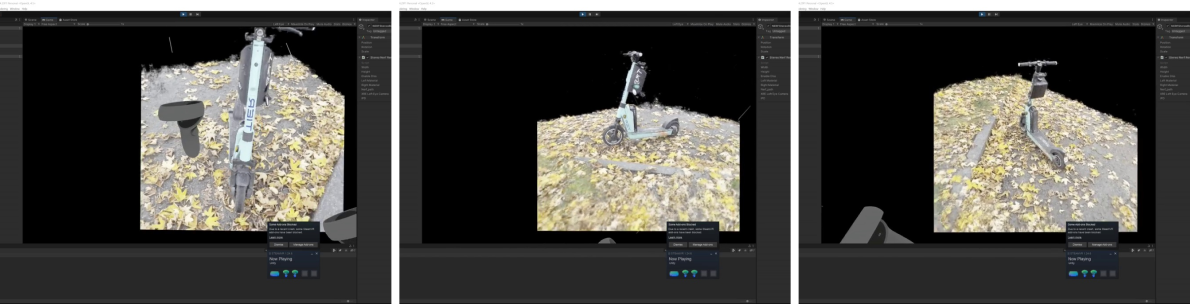
\includegraphics[width=\textwidth]{figures/tier_vr.png}
    \caption{NeRF viewed in VR with the help of immersive-ngp \cite{immersive-ngp}}
    \label{fig:tier_vr}
\end{figure}


% From Discord thread
\begin{comment} 
\textbf{Wavy artifacts in Nerfacto:}
AFAIK those wavy artifacts are from how the nerfacto model does ray sampling. Sometimes for very thin objects, none of the samples across a ray will land on it, causing it not to be visible in the rendering 

\textbf{Better results with another model?}
One of the reasons nerfacto is so fast is because it learns the distribution of weight across a ray, then samples from that distribution to get the ray samples. This means you aren't sampling where you don't need to, but also you might miss thin structures. Other methods might use more simple ray samplers that would densely sample across the ray, but would end up being a good bit slower to train/render
\end{comment}
\chapter{Discussion}
This chapter discusses and analyzes the results of the experiments, highlighting their significance in the context of the research questions. Additionally, the limitations of the thesis are discussed.

\section{Experiment 1: Defining a Baseline}

\begin{comment}
Points to discuss:
- Main point: Discuss the process of choosing which experiments was chosen.
- There might have been other experiments that should've been included in deciding the baseline.
- The way to choose which experiment goes forward could've been done differently.
- Although one experiment seem to do better with the current chosen setup, it might've done worse in another setup.
\end{comment}

In order to define a baseline for capturing data for training NeRFs, five experiments were selected and conducted: camera setup, capacity, number of frames, image resolution, and vehicle speed. These experiments were chosen based on heuristics and knowledge of what contributes to good NeRF results, such as well-lit scenes and non-blurry images. While the chosen experiments clearly consider important factors for capturing data for NeRFs, there may have been other experiments that could have been included in defining the baseline. It is also important to weigh the fact that the best-performing settings in one experiment may not generalize to other setups. Overall, the process of defining a baseline is an iterative one that requires careful consideration of various factors and a willingness to continuously improve and refine the baseline.

\subsection{Experiment 1.1: Camera Setup}
The results of the experiment showed relatively little difference in the quantitative metrics across the camera setups tested. However, the camera setup with two cameras at -10$^{\circ}$ and 10$^{\circ}$ yaw produced the highest \acrshort{ssim} and lowest \acrshort{lpips} scores, indicating that it produced the most visually similar and perceptually pleasing images. A possible explanation for why this specific camera setup produces the best results is the level of overlap between the captured images the respective camera setup provides. Both cameras have a \acrshort{fov} of $90^\circ$ and are mounted in the same location, resulting in a $70^\circ$ overlap between the images in the training data. This overlap entails that when the model trains on an image from one of the cameras, it necessarily also trains on approximately three-quarters of the scene captured from the other camera. Because the evaluation set is a subset of the training images, it is fair to assume that the model should score high on the respective metrics.

The camera setups used in the experiment were arbitrary and may not reflect how cameras are typically rigged on cars. Future research could explore more realistic camera setups to improve the generalizability of the results. Additionally, the camera setups used in the study were sparse, with only a few cameras at specific angles. It is possible that other camera setups could yield even better results.


\begin{comment}
- The position of the camera was arbitrary. Could've done more research into how cameras on cars usually are rigged.
- The camera setups are very sparse, a lot of different possibilities.

Results:
- Relatively little difference in the quantitative results.
- Why did the -10 and 10 yaw yield the best SSIM and LPIPS?
- The evaluation images are a subset of the training images. Because the -10 and 10 have a lot of overlap, they have a lot of common training data which will allow the model to learn the scene which it is evaluated on, in turn yielding high scores on the chosen metrics.


This overlap allows the model to train and learn the scene which it is evaluated on, because the evaluation set is a subset of the training images, more than the other setups, and it'll naturally score high on the respective images.

the model to train on the partial scene with two times the amount of data, and since the evaluation set is a subset of the training images, it'll naturally score high on the respective images.

\end{comment}










\subsection{Experiment 1.2: Capacity} 
% Summarize the important discussion added in the experiment
As stated in the experiment's section, the longest segment was selected for the baseline despite achieving the lowest scores across the metrics. This choice was made to ensure that the scene encompasses a diverse range of environments, including straight roads, curves, intersections, and varying lighting conditions.

% New discussion
In the qualitative analysis of the capacity results, it is evident that the quality of the renders degrades as the segment's length increase. The most prominent deterioration is the increase in blur; however, the \acrshort{psnr} remains relatively constant across the different experiments. A reason for this could be that \acrshort{psnr} has been shown to poorly capture the effects of blur \cite{videoprocessingai}, as exemplified by \autoref{fig:psnr-critique}. This example demonstrates the importance of evaluating the model across different metrics, as both \acrshort{ssim} and \acrshort{lpips} are good metrics for capturing blur.

\begin{figure}[ht]
    \centering
    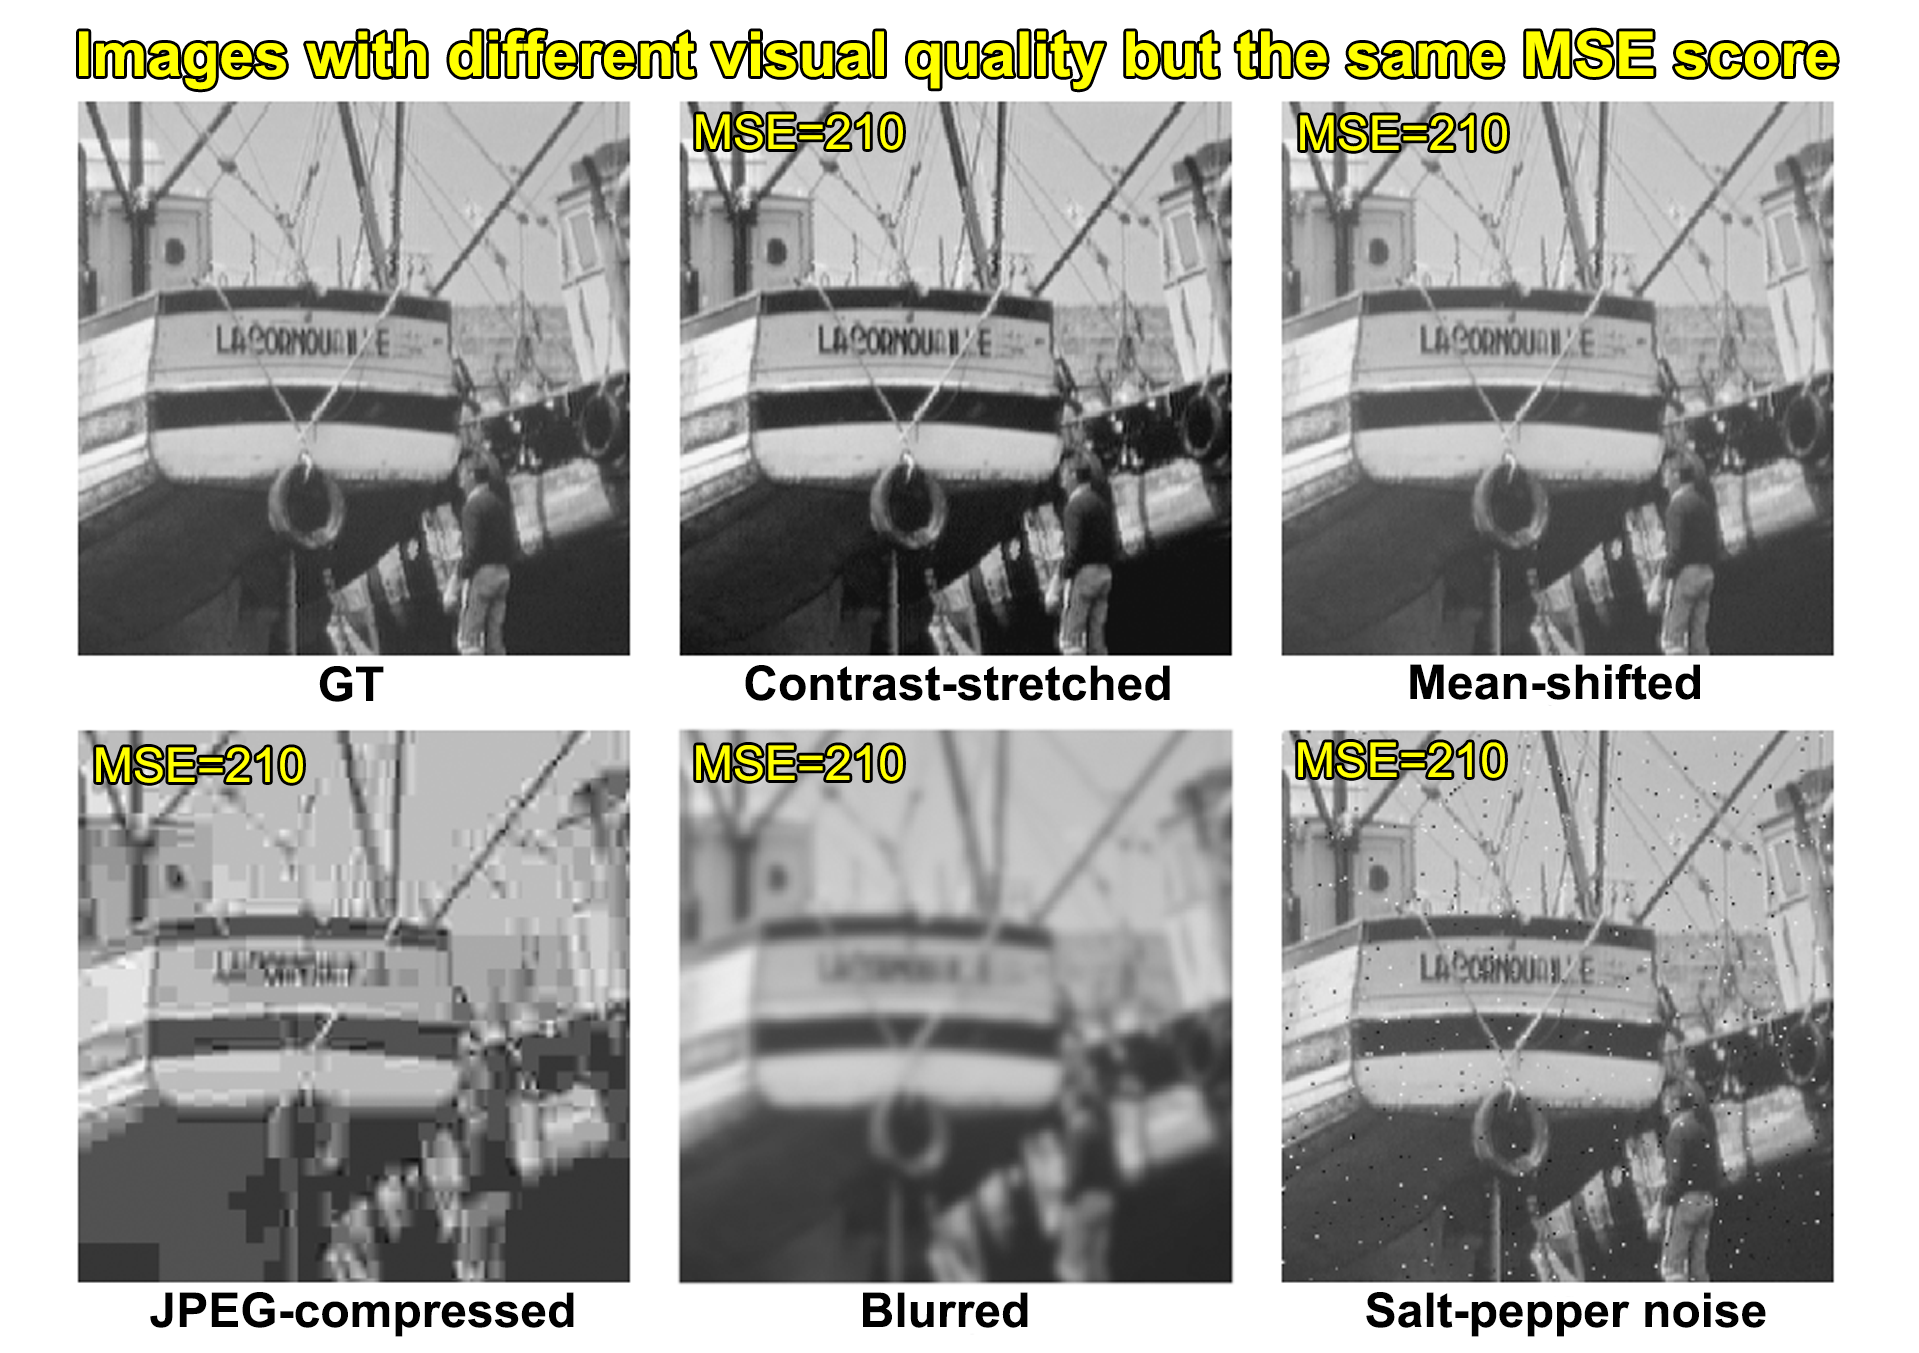
\includegraphics[width=1.0\textwidth]{figures/psnr-critique.png}
    \caption{Comparison of an image depicting a boat that has been subjected to various types of distortions.}
    \label{fig:psnr-critique}
\end{figure}

















\subsection{Experiment 1.3: Number of Frames}

%- The captured images are very similar
%- The default dataset size in Nerfstudio is 300 images
%- Show a mathematical proof of why more images would make sense

To comprehend the outcomes of this experiment, it would be beneficial to look into how the number of frames and the image resolution impact the training process. As detailed in the implementation details in \autoref{sec:nerfstudio-train-parameters}, the model is trained for 15'000 iterations where each iteration uses 4096 pixels. This results in $\sim61$ million pixels being sampled throughout a single training. With 225 training images and an image resolution of $600 \times 450$, $\sim61$ million pixels would be sampled. That means that by the end of the training, approximately all of the input pixels were trained on. A dataset containing more than 225 training images and corresponding camera poses would leave abundant pixels, and any fewer would lead to pixels being trained on multiple times. This calculation entail that the results should be relatively similar for all the conducted experiments with 1231, 615, 411, 307, and 247 images respectively. But, there is a significant drop in \acrshort{psnr} from experiments 1 to 4. The drop in \acrshort{psnr} indicates that another important factor is the variety in the dataset.


% TODO: I should discuss other options as to why the number of frames affect the metrics in the way it does.












\subsection{Experiment 1.4: Image Resolution}
Based on the metric scores, it might seem counterintuitive that the lowest resolution of $200 \times 150$ performed best. However, a deeper look into the qualitative results in \autoref{fig:image-size-comparison} reveals a different narrative. Despite lower resolutions yielding higher scores on metrics, they seem to fail in capturing fine-grained details, resulting in less visually pleasing images. On the other hand, higher-resolution images allow the NeRF to capture and replicate more intricate details, leading to superior visual outcomes, albeit with lower metric scores. This difference can be attributed to the higher sensitivity of metrics to minor discrepancies and noise in high-resolution images, potentially causing significant metric score reductions despite only minimal perceptual differences.

Given these considerations, the chosen resolution of $400 \times 300$ for the following experiments is a balanced choice, considering both the quantitative and qualitative results. Furthermore, it aligns well with the chosen number of frames from the \hyperref[sec:exp-number-of-frames]{Experiment 1.3}, as the combined configuration will allow training to sample about 84\% of the input pixels.

\begin{comment}
The qualitative assessment shows clear evidence of higher resolution images leading to higher fidelity renders, although the metrics suggest otherwise. When using lower-resolution images, the metrics may become less sensitive because they are less affected by small differences between the synthesized and ground-truth images. This is because lower-resolution images have fewer pixels, which can make the metrics less precise in measuring the perceptual similarity between the images. However, using lower-resolution images can also lead to a loss of detail and fidelity in the synthesized images. When comparing low-resolution images with high-resolution images, these metrics may become less effective because the high-resolution images are more sensitive to small differences between the synthesized and ground-truth images. In other words, the NeRF may generate high-quality images that are perceptually similar to the ground-truth images, but small differences in the pixel values or noise can cause a significant decrease in the metric scores.

The chosen resolution of $400 \times 300$ aligns well with the chosen number of frames from the previous experiment. With 2 ticks per image, $\sim615$ images for the baseline, we have $\sim73$ million pixels. The training will cover about 84\% of the input pixels.

This might be a special case for synthetic data where we have perfect camera poses. With higher-resolution images, the requirement for accurate camera poses increases as the camera poses have to be aligned pixel perfect with the image.
\end{comment}












\subsection{Experiment 1.5: Vehicle Speed}
The reason why the runs with higher vehicle speeds achieve worse results might be attributed to the motion blur and temporal artifacts that can occur when the vehicle is moving fast. In CARLA these effects are added as part of the post-processing of the captured camera image. At higher speeds, the motion of the vehicle can cause blurring and distortion in the captured images, which can reduce the quality of the data and make it more difficult for the NeRF to learn the underlying 3D scene structure and appearance. In contrast, slower vehicle speeds can reduce the amount of motion blur and temporal artifacts, resulting in clearer and more detailed images. 

Another side effect of driving slower is that it leads to an increased amount of images captured. At 50\% speed, the dataset consists of 1095 images, in contrast to the 429 images captured at 200\% speed. An increased dataset size proved to be beneficial in \hyperref[sec:exp-number-of-frames]{Experiment 1.3}, and could positively affect the results in this experiment.


% The reason for this can be attributed to the motion blur and temporal artifacts that can occur when the vehicle is moving too fast. At higher speeds, the motion of the vehicle can cause blurring and distortion in the captured images, which can reduce the quality of the data and make it more difficult for the NeRF to learn the underlying 3D scene structure and appearance. In contrast, slower vehicle speeds can reduce the amount of motion blur and temporal artifacts, resulting in clearer and more detailed images. Another side effect of driving slower is that it leads to increased amount of images captured. At 50\% speed, the dataset consists of 351 images, in contrast to the 131 images captured at 200\% speed.
























\subsection{Experiment 1.6: Assessing the Combined Baseline}
% I might not need the initial "Defining a baseline" if I sum it up in this chapter.
\begin{description}[leftmargin=!,labelwidth=\widthof{RQ 1:}]
\item[\textbf{RQ 1:}] What are the critical factors that need to be considered when capturing synthetic data for training NeRF models, and how do they impact the performance of the resulting models?
\end{description}


From the experiments discussed above, it is evident that all the configurations contribute to the quality of the data capture, which in turn contributed to the quality of the image synthesis from the resulting NeRF. Nevertheless, it is challenging to quantify the extent to which each of the different configurations affects the quality of the final baseline results.

Looking at the experiments separately, image resolution had the largest span between the quantitatively best and worst metrics. Nevertheless, the qualitative results indicated that the quantitative comparison did not convey a fair comparison of the render-quality. Due to this, the capacity-experiment could be the experiment with the most impact on the final result.

In conclusion, when capturing synthetic data for training NeRF models, it is important to consider the camera setup, segment length or scene size, dataset size, image resolution, and vehicle speed. Each of these parameters presents unique influences on the quality of the data captured, and in turn, the performance of the resulting NeRF models.


\begin{comment}
The critical factors that must be considered when capturing synthetic data for training NeRF models, as inferred from the discussed baseline experiments, encompass camera setup, capacity, number of frames, image size, and vehicle speed. Each of these factors demonstrates a unique impact on the performance of the resulting models.

Camera setup plays a significant role in determining the quality of data captured for NeRF models. The experiments revealed that certain camera arrangements, specifically a setup with two cameras at -10$^{\circ}$ and 10$^{\circ}$ yaw, can result in superior SSIM and LPIPS scores, indicating more visually similar and perceptually pleasing images. This finding can be attributed to the degree of overlap between images captured by each camera in the setup. However, the experiments also highlight that camera arrangements were arbitrary and future research may investigate more realistic setups to better generalize the results.

The capacity, or the length of the road segment covered, also impacts the performance of the NeRF models. Even though longer segments led to lower scores across the metrics, these were still selected as the baseline to ensure a diverse range of environmental exposure for the model. It was noticed that the quality of renders deteriorated, especially in terms of increased blur, as segment length increased. Hence, the capacity of data has implications on the clarity and diversity of the training set, which could potentially influence the robustness of the model to diverse scenarios.

The number of frames in the dataset is another crucial factor. An optimal balance between the number of images and the image resolution is important for efficient training. In the experiments, a dataset with 225 images, each with a resolution of $600 \times 450$, covered approximately all of the input pixels by the end of training. However, a dataset with too many or too few images could result in either underutilization or overutilization of the pixels during training. Additionally, a decrease in PSNR with a drop in the number of frames points to the role of variety in the dataset.

The size of the images, or their resolution, has a complex impact on model performance. While higher resolution images contribute to higher fidelity renders, the metrics could suggest otherwise due to their increased sensitivity to minor differences in synthesized and ground-truth images. Hence, resolution can impact the quality of synthesized images and their metric scores, and it is crucial to align it with the number of frames for efficient coverage of input pixels.

Vehicle speed is a significant factor when capturing synthetic data, particularly due to the influence of motion blur and temporal artifacts on image quality. Faster vehicle speeds can lead to increased blur and distortion, making it challenging for the NeRF to learn the scene structure and appearance. Conversely, slower speeds provide clearer and more detailed images, improving the quality of the training data. Furthermore, slower speeds result in a larger dataset due to the increased number of images captured.

In conclusion, each of these factors—camera setup, capacity, number of frames, image size, and vehicle speed—has a unique and important influence on the quality of synthetic data captured for training NeRF models. Their careful consideration is essential for optimizing the performance of the resulting models.
\end{comment}








\section{Experiment 2: Simulated Noise Conditions}
\begin{description}[leftmargin=!,labelwidth=\widthof{RQ 1:}]
\item[\textbf{RQ 2:}] How does the initial camera pose accuracy and segment length impact the final reconstruction? Can rough initial camera poses be optimized to achieve comparable results to those obtained from tools such as COLMAP?
%How does the accuracy of initial camera poses and segment size influence the effectiveness of camera pose optimization, and is it possible to achieve equivalent results by optimizing rough camera poses directly, as opposed to pre-processing an approximation of accurate camera poses with tools such as COLMAP?
\end{description}

This research question addresses the effects of imperfect camera poses, frequently encountered in real-world scenarios due to \acrshort{gps}/\acrshort{gnss} inaccuracies, on the performance of camera pose optimization. We examine this by adding Gaussian noise to camera poses obtained from the CARLA pipeline, simulating real-world inaccuracies in these camera poses.

Despite Gaussian noise not perfectly replicating real-world noise distributions, its application allows an indicative examination of camera pose optimization within the Nerfacto-pipeline. It is noteworthy that while the quantitative distinction between the non-optimized and optimized camera pose results might appear marginal, the qualitative contrasts depicted in \autoref{fig:noise-combined-comparison} deliver strong evidence of the camera pose optimization's effectiveness.

Particularly, the qualitative comparison highlights that the optimized camera poses generate consistently higher quality renders, even under significant noise levels. This is more noticeable within shorter segments, where the optimization seems more efficient than in the larger baseline scene. This finding may be attributed to the previously discussed limitations in capacity, given that the camera optimization treats camera pose parameters as jointly optimized learnable parameters along with the RGB values.

Interestingly, the only instance where non-optimized poses yield superior results is when no noise is introduced. In such cases, the resulting render from non-optimized camera poses appears considerably sharper than its optimized counterpart, which appears comparatively more blurred. This outcome is likely unique to datasets with near-perfect camera poses, such as the synthetic dataset used in this experiment.


When examining the effectiveness of COLMAP pre-processing against the joint optimization of initial camera poses along with the other learnable parameters, it becomes evident that COLMAP tends to deliver superior performance. This observation holds particularly when the initial rough camera poses are influenced by a rather minor noise adhering to a Gaussian distribution with a standard deviation of $0.1^2$. Under these conditions, all three evaluation metrics (\acrshort{psnr}, \acrshort{ssim}, \acrshort{lpips}) associated with the NeRF lag behind those achieved by COLMAP, as can be seen from \autoref{tab:exp-gaussian-noise} and \autoref{tab:colmap-vs-poses}. Furthermore, when the noise's standard deviation is escalated to $0.5^2$, which is fair to assume could occur during real-world data capture, the metrics degrade even more significant compared to what COLMAP can deliver. While the processing time required by COLMAP might seem prohibitively lengthy for large datasets, this concern can be addressed by splitting the data into smaller sections. Thus, despite the initial time investment, COLMAP's superior performance merits consideration, particularly in scenarios with significant noise in initial camera poses.

\begin{comment}
The horizontal and vertical vectors in each experiment are subject to equal Gaussian noise. This approach may not fully capture the variability in noise that arises from realistic data capture scenarios, where factors such as the direction and speed of the vehicle can affect noise distribution. Nevertheless, the use of Gaussian noise enables the evaluation of the impact of camera optimization in the Nerfacto-pipeline.

While the difference in quantitative results between the runs with- and without camera pose optimization appear small, the qualitative comparison depicted in both \autoref{fig:noise-short-segments} and \autoref{fig:noise-baseline-segments} provides compelling evidence of its efficacy. Contrary to the NeRF that doesn't optimize the camera poses, the renders from the NeRF that optimized the camera poses remain relatively high-quality even when there is a substantial amount of noise added. This is particularly noticeable on shorter segments, where the optimization appears to perform even better than on the larger baseline scene. The observation can likely be ascribed to the capacity limitations previously discussed. This is because the camera optimization approach treats the camera pose parameters as learnable parameters that are jointly optimized with the RGB values.

The only scenario where NeRF with non-optimized camera poses outperforms its optimized counterpart is when no noise is added. In such cases, the resulting render is notably sharper than that produced by the optimized NeRF, which can appear more blurred. This finding is likely exclusive to synthetic datasets with perfect camera poses.
\end{comment}


\begin{comment}
DON'T NEED THIS SECTION BECAUSE THE COLMAP-RESULTS ARE DISCUSSED IN COMBINATION WITH THE NOISE-EXPERIMENT ABOVE.

\section{COLMAP vs. Absolute poses}
From the quantitative results, it appears COLMAP optimizes the camera poses similar to the camera pose optimization step in the Nerfacto-pipeline. When we turn off the camera pose optimization step, the perfect poses from CARLA enable even higher scores across the metrics and sharper renders.
\end{comment}





\section{Experiment 3: Comparing NeRF-models}
\begin{description}[leftmargin=!,labelwidth=\widthof{RQ 1:}]
\item[\textbf{RQ 3:}] How do different NeRF methods (Instant-ngp \cite{muller_instant_2022}, Mip-NeRF \cite{barron_mip-nerf_2021}, Nerfacto \cite{tancik_nerfstudio_2023}) perform on unbounded scenes in terms of reconstruction quality and computational efficiency?
\end{description}

Upon examination of the different NeRF methods, namely Nerfacto, Instant-ngp, Nerfacto-big, and Mip-NeRF, it is evident that their performance in terms of reconstruction quality and computational efficiency on unbounded scenes is rather comparable, with the exception of Mip-NeRF.

Both Nerfacto and Instant-ngp demonstrate high performance on the evaluated metrics, showcasing their proficient ability to effectively learn and represent the unbounded scene. The largest deviation between the two models is their \acrshort{lpips} score, where Nerfacto outperforms Instant-ngp. Nerfacto-big is a differently configured Nerfacto-model featuring, among other configurations presented in \autoref{tab:nerfacto-big-parameter-overview}, an expanded hidden layer width which increases the model's capacity. Despite being trained for a significantly larger number of iterations it fails to exceed the performance of its less complex counterparts.

Mip-NeRF, which is designed for bounded scenes, predictably falls short in learning the unbounded scene. It yields the lowest scores across all metrics. The qualitative evaluation further support this, showing no perceivable scene structure in its renderings, despite producing some correct color representations.

Given these findings, Nerfacto emerges as a strong candidate for subsequent experiments. Furthermore, it should serve well as a backbone-model for applications to build upon, thanks to its balance between reconstruction quality and computational efficiency.



\section{Experiment 4: Large-Scale NeRF}
\begin{description}[leftmargin=!,labelwidth=\widthof{RQ 1:}]
\item[\textbf{RQ 4:}] What are the technical challenges and considerations for implementing a functional approach for large-scale NeRF within the Nerfstudio API, and how does it compare to approaches not optimized for large-scale in terms of scalability, efficiency, and rendering quality?
\end{description}

Implementing a functional approach for large-scale NeRF within the Nerfstudio API has been technically challenging, as elaborated upon in \autoref{sec:method-block-nerf}. However, the initial naive Block-NeRF approach has displayed encouraging performance in both quantitative and qualitative aspects. The experimental results confirm that compared to training single NeRFs on large scenes, the Block-NeRF approach yields superior outcomes. The image synthesis produced by the Block-NeRF approach exhibits sharper details and an overall enhancement in the visual quality.

While the naive implementation of Block-NeRF does not inherently exhibit optimal scalability, it holds significant potential for improvement. In its current state, each Block-NeRF is trained sequentially, creating a bottleneck that limits scalability. However, the architecture provides an opportunity for horizontal scaling, which could be achieved by parallelizing the unique training processes across multiple \acrlong{gpu}s (\acrshort{gpu}s). This adjustment would drastically improve efficiency and reduce training time, thereby enhancing scalability.

Nevertheless, it is important to acknowledge that this process is computationally intensive, and care should be taken to find a balance between the quality of the results and the efficiency of the process. Future work could focus on optimizing this balance to make large-scale NeRF more viable and efficient, while maintaining the high-quality image synthesis that the Block-NeRF approach has demonstrated thus far.





\subsection{Experiment 4.1: Removing Artifacts}
%The overlap between the blocks become substantially less visible with higher overlap values, $\delta$. When we increase $\delta$, we increase the dataset of each block leading to the capacity issue previously explored. In a production setting, it'll be important to tune all these parameters to effectively maximize quality across all blocks.

The introduction of an overlap $\delta$ between the naive Block-NeRF's data resolves the problem of visible artifacts during the transition between Blocks. However, as $\delta$ increases, the dataset size for the respective Block-NeRFs increase, and the collective render quality decreases. This finding is consistent with the results from \hyperref[sec:exp-capacity]{Experiment 1.2}, which indicate that the scene size is inversely correlated with render quality.

While the approach of incorporating overlap between the Block-NeRF's data resolves the problem of visible artifacts during the transition between Blocks, it is evident from \autoref{fig:block-nerf-frame-comparison} that the final frame rendered by a Block-NeRF produces renders of lower quality compared to the initial frame rendered by the same Block-NeRF. If the second Block-NeRF's dataset contains images captured closer to the respective motive, indicating more detailed images, this difference is to be expected. However, the difference could potentially be mitigated by experimenting with image-merging techniques, for example, by rendering the view from both blocks and merging them with techniques like \textit{inverse distance weighing}.

%Further improvements that could be done:
%- The details of the scenery in the second frame is clearly better than the first, which is expected as block number 2 has been trained on close-up images of the scene. This difference could be mitigated by looking into image-merging techniques such as inverse distance weighing.



\section{Experiment 5: Real Data}
The naive Block-NeRF approach emerges as the clear frontrunner in the experiments on real data, producing both the best quantitative and qualitative results. This finding aligns with expectations considering the scale of the scene being learned, which potentially surpasses the capacity of a single NeRF. Among all conducted experiments, the Block-NeRF run, with camera poses approximated by COLMAP without further optimization, demonstrated a distinct supremacy across all metrics, affirming the advantage of COLMAP-based pose estimation over \acrshort{gps}-derived alternatives.

In the subset of experiments excluding the naive Block-NeRF approach, the approach utilizing COLMAP without subsequent optimization yielded the best results. Among the runs with camera poses estimated from \acrshort{gps}-readings, those involving subsequent camera pose optimization produced superior metrics. These findings further support the observation that camera poses that are near-perfect tend to be disadvantaged by subsequent optimization, while imperfect camera poses benefit from this process. This observation is further reinforced by the qualitative evaluation of the different runs, presented in \autoref{fig:trip086-comparison}, where the output from runs utilizing near-perfect camera poses tended to exhibit blurriness upon subsequent optimization. In contrast, the use of subsequent optimization of imperfect camera poses enabled the NeRF to generate more precise and clear renderings.



\begin{comment}
% Discuss the implementation of rotation matrix
- The estimation could be further improved by investigating techniques for leveraging more of the contained data.
- The NAPLab car's accelerometer could be used to calculate roll and pitch.
- LiDAR data could be used for further pose estimation
\end{comment}





\section{Experiment 6: Novel Views Along Altered Trajectory}
One of the benefits of using NeRFs for training \acrshort{ad} systems, is the ability to generate data along altered trajectories. While this can be achieved with a simulator, as discussed in \autoref{sec:wayve}, the application of NeRF becomes particularly useful when a high-quality NeRF has been trained on real data. In addition to evaluating the autonomous vehicle in a novel environment, the NeRF can be used to expand the training dataset for the autonomous vehicle by creating an arbitrary number of altered camera paths and synthesizing photo-realistic novel views of altered trajectories. This can help improve the robustness and generalizability of the \acrshort{ad} system by exposing it to a wider range of scenarios and viewpoints.

Looking into the experimental results from \hyperref[sec:altered-trajectories]{Experiment 6}, it is important to note that the absence of ground truth images from the altered path inherently constrains the ability to conduct quantitative analysis beyond the initial evaluations. The qualitative assessment is thus the primary mode of evaluation. From the renderings depicted in \autoref{fig:altered-trajectories}, we can clearly see the potential of this application. Although the novel-rendered perspectives do not always match the quality and coherence found in the original evaluation images, they are largely successful in producing clear and structurally accurate visualizations. This affirms their potential and the effectiveness of the approach.



\section{Shortcomings}
Several areas of potential improvement can be recognized within this study. Firstly, while the research has illuminated key aspects of data capture from vehicles, the time constraints of the project did not allow us to validate these findings through real-world testing. Synthetic data sets were leveraged extensively and provided evidence that the combined configurations for the baseline were promising. However, the validity of these results has yet to be confirmed in real-world capture.

Secondly, there exist limitations in the capture of real data, specifically in the estimation of transformation matrices. The camera poses' translational components are derived from raw \acrshort{gnss}-readings, and the rotational components are estimated through trigonometric comparisons of adjacent \acrshort{gnss}-readings. Such a method is inherently susceptible to errors and inaccuracies. To improve the accuracy and reliability of data capture, a better approach could be to utilize both of the vehicle's \acrshort{gnss} sensors and integrate the vehicle's accelerometer data to achieve precise roll and pitch estimations.
\chapter{Conclusion \& Future Work}

\section{Conclusion}
Conclude the thesis. Could create a holistic research goal that I could use to wrap up the thesis, or I could conclude what has been done, what worked and what should be looked into.



















\section{Future Work}
This section provides ideas related to NeRFs, synthetic data capture, and the extension to real-life data capture that were not covered in this report, but would be interesting to explore in future work.

\subsection{Improve pipeline for real-data capture}
Better estimate the rotation matrix from the collected data

\subsection{Large scale NeRF}
\begin{comment}
- Create a pipeline that enables the use of COLMAP for each segment in a more streamlined way. A succesful implementation should have significant implications on the quality of the resulting render.
- Mask transient objects using segmentation models
- Inverse distance weighing
- Visibility prediction
- Change backbone model to a model like F2 which have a different space warping algorithm, and should enable better results than using Nerfacto as the backbone model.
\end{comment}

\begin{itemize}
    \item Create a pipeline that enables the use of COLMAP for each segment in a more streamlined way. A successful implementation should have significant implications on the quality of the resulting render.
    \item Mask transient objects using segmentation models.
    \item Inverse distance weighing.
    \item Visibility prediction.
    \item Change backbone model to a model like F2 which has a different space warping algorithm, and should enable better results than using Nerfacto as the backbone model.
\end{itemize}

%\chapter{Using the Document Class}
\label{chap:usage}

\section{Thesis Setup and Language Selection}
\label{sec:setup}

The document class is initialized by issuing the \texttt{\textbackslash documentclass[]\{ntnuthesis\}} at the beginning of your \texttt{.tex} file. The thesis language should be given as an option. Currently British English (class option \texttt{[british]}), American English (class option \texttt{[american]}), Norwegian Bokmål (class option \texttt{[norsk]}) and Norwegian Nynorsk (class option \texttt{[nynorsk]}) are supported.\footnote{Disclaimer: this unfortunate naming of the Norwegian language options follows from the naming conventions of the \texttt{babel} package.}

There is also the \texttt{titlepage} class option that triggers the generation of a simple title page that can be used as a placeholder when writing the thesis. This option should be removed before handing in the thesis. Instead the official NTNU titlepage for the corresponding thesis type should be added as described on Innsida.\footnote{see \url{https://innsida.ntnu.no/wiki/-/wiki/English/Finalizing+the+bachelor+and+master+thesis} for bachelor and master, and \url{https://innsida.ntnu.no/wiki/-/wiki/English/Printing+your+thesis} for PhD.}

\section{Title, Author, and Date}

In the preample of the \texttt{.tex} file, the thesis title should be set with the \texttt{\textbackslash title\{\}} command. The title will appear on the titlepage as well as in the running header of the even numbered pages. If the title is too long for the header, you can use \texttt{\textbackslash shorttitle\{\}} to set a version for the header.

The authors should be listed with full names in the \texttt{\textbackslash author\{\}} command. If there are several authors, they should be separated with \texttt{\textbackslash and}, e.g., like this: \texttt{\textbackslash author\{Anne Andersen \textbackslash and Bjørn Bjørnsen\}}. For the running headers, you may want to use \texttt{\textbackslash shortauthor}, e.g. like this: \texttt{\textbackslash shortauthor\{A. Andersen and B. Bjørnsen\}} or even \texttt{\textbackslash shortauthor\{Andersen et al.\}}.

Use \texttt{\textbackslash date\{\}} to set the date of the document. It will only  appear on the temporary title page. To keep track of temporary versions, it can be a good idea to use \texttt{\textbackslash date\{\textbackslash today\}} while working on the thesis. You may also add copyright and licence information in this field.

\section{Page Layout}

The document class is designed to work with twosided printing. This means that all chapters start on odd (right hand) pages, and that blank pages are inserted where needed to make sure this happens. However, since the theses are very often read on displays, the margins are kept the same on even and odd pages in order to avoid that the page is jumping back and forth upon reading.

To avoid blank pages when rendering the thesis, you can enable the \texttt{oneside} option in the \texttt{thesis.tex} file. Just add 'oneside' to the document class options on the first line, and recompile.

\section{Structuring Elements}

The standard \LaTeX{} elements for document structure are supported: chapter, section, and:

\subsection{This is a \texttt{\textbackslash subsection\{\}}}

Short subsection text here.

\subsubsection{This is a \texttt{\textbackslash subsubsection\{\}}}

Short subsubsection text here.

\paragraph{This is a \texttt{\textbackslash paragraph\{\}}}

Short paragraph text here.

Chapters, sections, and subsections will be included in the table of contents, whereas the lower level structuring elements will not appear there. Don't use too many levels of headings; how many are appropriate, will depend on the size of the document. Also, don't use headings too frequently.

Make sure that the chapter and section headings are correctly capitalised depending on the language of the thesis, e.g., `\emph{Correct Capitalisation of Titles in English}' vs. `\emph{Korrekt staving av titler på norsk}'.

Simple paragraphs are the lowest structuring elements and should be used the most. They are made by leaving one (or more) blank line(s) in the \texttt{.tex} file. In the typeset document they will appear indented and with no vertical space between them.

\section{Lists}

Numbered and unnumbered lists, i.e., the \texttt{enumerate} and \texttt{itemize} environments, are used just as in regular \LaTeX{}, but are typeset somewhat more densely and with other labels. Unnumbered list:
\begin{itemize}
    \item first item
    \item second item
    \begin{itemize}
        \item first subitem
        \item second subitem
        \begin{itemize}
            \item first subsubitem
            \item second subsubitem
        \end{itemize}
    \end{itemize}
    \item last item
\end{itemize}
Numbered list:
\begin{enumerate}
    \item first item
    \item second item
    \begin{enumerate}
        \item first subitem
        \item second subitem
        \begin{enumerate}
            \item first subsubitem
            \item second subsubitem
        \end{enumerate}
    \end{enumerate}
    \item last item
\end{enumerate}

For description lists, see usage in, e.g., \cref{sec:frontmatter}.

\section{Figures}

Figures are placed in the \texttt{figure} environment. An example is shown in \cref{fig:mapNTNU}. Figures are floats, hence they will float freely around in the document in accordance with standard \LaTeX{} behaviour. You may want to try to override \LaTeX{}'s default placement by using the \texttt{h} (here), \texttt{t} (top of page), \texttt{b} (bottom of page), and \texttt{p} (separate page) options in order of priority. If you provide an alternate (typically shorter) caption in square brackets, it will be used in the list of figures. Use \texttt{\textbackslash includegraphics[]\{\}} with options \texttt{scale} or \texttt{width} to include the graphics file. The caption should be placed \emph{below} the figure. If the caption consists of a single sentence fragment (incomplete sentence), it should not be punctuated. Given the shape and size of the figure, the figure caption can appear too close or too far from the figure. To deal with this, vertical space, either positive or negative, can be added before and/or after the caption command using the \texttt{\textbackslash vspace{}} command.

\begin{figure}[htbp]  % order of priority: h here, t top, b bottom, p page
  \centering
  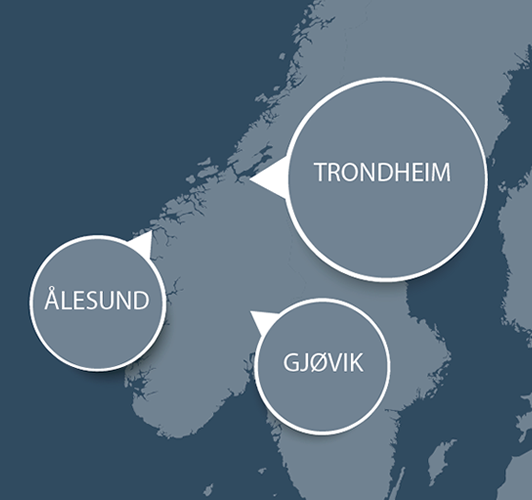
\includegraphics[width=.5\textwidth]{figures/kart_student}
  \caption[Map of NTNU Campuses]{The map shows the three main campuses of NTNU.}
  \label{fig:mapNTNU}
\end{figure}

For figures compsed of several sub-figures, the \texttt{caption} and \texttt{subcaption} packages have been preloaded. See \cref{fig:subfig} with \cref{sfig:a,sfig:b} for an example. For more details on alignment etc., see the Overleaf documentation.\footnote{\url{https://www.overleaf.com/learn/latex/How_to_Write_a_Thesis_in_LaTeX_(Part_3):_Figures,_Subfigures_and_Tables}}

\begin{figure}
    \centering
    \begin{subfigure}[b]{.45\textwidth}
        \centering
        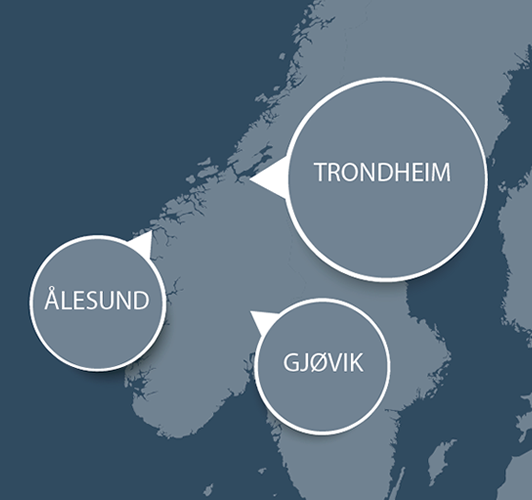
\includegraphics[width=\textwidth]{figures/kart_student.png}
        \caption{First sub-figure}
        \label{sfig:a}
    \end{subfigure}
    \hfill
    \begin{subfigure}[b]{.45\textwidth}
        \centering
        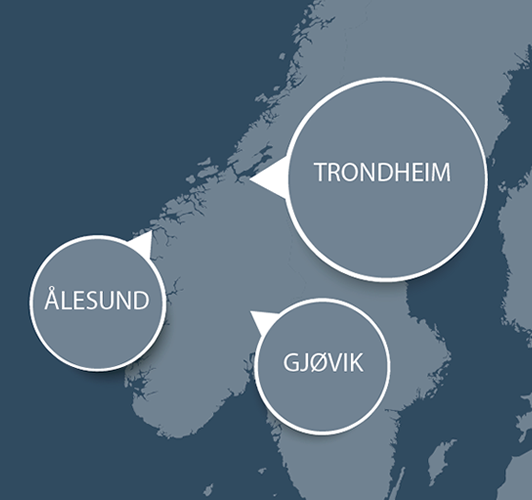
\includegraphics[width=\textwidth]{figures/kart_student.png}
        \caption{Second sub-figure}
        \label{sfig:b}
    \end{subfigure}
    \caption{A figure composed of two sub-figures. It has a long caption in order to demonstrate how that is typeset.}
    \label{fig:subfig}
\end{figure}

You can make nice graphs directly from data files using \texttt{gnuplot}, but it is expensive on every compilation.  The code is included in the
raw latex as a comment so you can uncomment that code to see how it works.
% , for an example, see \cref{fig:examplegnuplot}.
%
%\begin{figure}[htbp]
%  \centering
%    \begin{gnuplot}[terminal=epslatex,terminaloptions={size 8cm,6cm color}]
%        set xlabel "age"
%        set ylabel "IQ"
%        set key autotitle columnhead
%        set title "age vs IQ"
%        set yrange [0:160]
%        set datafile separator ","
%        plot "csvtables/ageiq.csv" using 1:2 with boxes
%    \end{gnuplot}
%  \caption[An example of Integrated Graph]{This is a gnuplot graph read from a file. Also this figure has a long caption in order to demonstrate how that is typeset.}
%  \label{fig:examplegnuplot}
%\end{figure}

\section{Tables}

Tables are placed in the \texttt{table} environment. An example is given in \cref{tab:example1}. Like figures, tables float freely around in the document in accordance with standard \LaTeX{} behaviour. The table caption should be placed \emph{above} the table. If the caption consists of a single sentence fragment (incomplete sentence), it should not be punctuated.

\begin{table}
  \centering
  \caption{A simple, manually formatted example table}
  \label{tab:example1}
  \begin{tabular}{cc}
    \hline
    age  & IQ \\
    \hline
    10   & 110 \\
    20   & 120 \\
    30   & 145 \\
    40   & 120 \\
    50   & 100 \\
    \hline
  \end{tabular}
\end{table}

Tables can also be automatically generated from CSV files using the \texttt{simplecsv} and \texttt{booktab} packages. See \cref{tab:examplecsv} for an example.

\begin{table}[tbp]
  \centering
  \caption[A simple example table generated from a CSV file]{A simple example table generated from a CSV file using \texttt{simplecsv} and \texttt{booktab}}
  \label{tab:examplecsv}
  \csvautobooktabular{csvtables/ageiq.csv}
\end{table}

\section{Listings}

Code listings are included by means of the \texttt{listings} package. Code examples can be read from file or provided inline, and should be given a caption for cross referencing and for appearance in the list of code listings in the thesis frontmatter. If all your code examples are written in the same programming language, you can use, e.g., \texttt{\textbackslash lstset\{language=Python\}} to set the language once and for all. The code is set with the monospace font, and the font size is reduced to allow for code lines up to at least 80 characters without causing line breaks. Options for programming languages, line numbering etc. are provided. Unlike figures and tables, code listings are not floating objects, and will appear at the same position in the typeset document as in the \texttt{.tex} file. If the caption consists of a single sentence fragment (incomplete sentence), it should not be punctuated.

\lstinputlisting[
    caption={Python example from file},
    label=lst:pythonfile,
    language=Python
]{listings/example.py}

\lstinputlisting[%
    caption={C++ example from file},
    label=lst:cppfile,
    language=C++,
    numbers=left
]{listings/example.cc}

\begin{lstlisting}[
    caption={Python code in \LaTeX{} document},
    label=lst:pythondoc,
    language=Python]
import numpy as np
import matplotlib.pyplot as plt

x = np.linspace(0, 1)
y = np.sin(2 * np.pi * x)

plt.plot(x, y)
plt.show()
\end{lstlisting}

\begin{lstlisting}[
    caption={C++ code in \LaTeX{} document},
    label=lst:cppdoc,
    language=C++]
#include <iostream>
using namespace std;

int main()
{
  cout << "Hello, World!" << endl;
  return 0;
}
\end{lstlisting}

\section{Equations}

Equations are typeset as normally in \LaTeX{}. It is common to consider equations part of the surrounding sentences, and include punctuation in the equations accordingly, e.g.,
\begin{equation}
    f(x) = \int_1^x \frac{1}{y}\,dy = \ln x\,.
    \label{eq:logarithm}
\end{equation}
For more advanced symbols like, e.g., $\mathbb{R}, \mathbb{Q}$, the \texttt{amssymb} package is preloaded, and for more advanced mathematical layout the \texttt{amsmath} behaviour is obtained through the \texttt{mathdesign} package. Confer the overleaf documentation for details.\footnote{\url{https://www.overleaf.com/learn/latex/Mathematical_expressions}}

\section{Fonts}

Bitstream Charter at 11pt with the corresponding Mathdesign math fonts have been selected as the main fonts for the thesis template. For code examples, the monospaced font should be used – for this, a scaled version of the DejaVuSansMono to match the main font is preselected. If you would like to use an accompanying sans serif font, the BeraSans has been made available. The standard \LaTeX{} font commands should be used to switch between fonts, e.g.,
\texttt{\textbackslash textit\{\}} \textit{for italics},
\texttt{\textbackslash textbf\{\}} \textbf{for bold face},
\texttt{\textbackslash texttt\{\}} \texttt{for mono spaced}, and
\texttt{\textbackslash textsf\{\}} \textsf{for sans serif}.
For generic \emph{emphasis}, \texttt{\textbackslash emph\{\}} should be applied.

\section{Cross References}
\label{sec:crossref}

For cross references, i.e., references within the document, the \texttt{\textbackslash cref\{\}} command provided byt the \texttt{cleveref} package should be used. Labels are inserted in the document in the standard \LaTeX{} manner. They are case sensitive, so, e.g., a label immediately after a section command refers to that section, while a label within, e.g., a table environment refers to the table. The \texttt{\textbackslash cref\{\}} command also generates the corresponding text. If the document is in English (class options \texttt{british} or \texttt{american}), the cross references are capitalised, whereas if it is in Norwegian (class options \texttt{norsk} or \texttt{nynorsk}), they are not. If you are writing in Norwegian, you should use \texttt{\textbackslash Cref\{\}} at the beginning of a sentence to ensure that the cross reference is correctly capitalised. For examples on usage, see \cref{sec:crossref} in \cref{chap:usage}, \cref{tab:example1}, \cref{fig:mapNTNU}, \cref{eq:logarithm}, \cref{lst:cppfile}, \cref{paper:scrutiny}, and \cref{app:additional}. \Cref{app:additional} at the beginning of a sentence.

The cross references are made into active hyperlinks in the resulting PDF document by the use of the \texttt{hyperref} package. The colour of the links is set to black for best appearance on print. This can easily be changed by the author by the use of the \texttt{\textbackslash hypersetup\{\}} command.

\section{Glossary and Acronyms}
The template comes with the ability to create a glossary and acronym list. To add entries to one of these lists, add them to the \texttt{glossary.tex} file.
All uses of the acronym and glossary functions will create a clickable link that references the corresponding entry in one of the lists. All entries in the lists will also contain page references to all places it has been used.
\subsection{Using Acronyms}
To render acronyms, you have three options:
\begin{itemize}
  \item \texttt{\textbackslash acrlong\{ \}} prints the phrase the acronym stands for, e.g. \texttt{\textbackslash acrlong\{gcd\}} displays \acrlong{gcd}.
  \item \texttt{\textbackslash acrshort\{ \}} prints the acronym, e.g. \texttt{\textbackslash acrshort\{gcd\}} displays \acrshort{gcd}.
  \item \texttt{\textbackslash acrfull\{ \}} prints both the acronym and its definition, e.g. \texttt{\textbackslash acrfull\{gcd\}} displays \acrfull{gcd}.
\end{itemize}

\subsection{Using Glossary}
\begin{itemize}
  \item \texttt{\textbackslash gls\{ \}} prints the term in lowercase, e.g. \texttt{\textbackslash gls\{maths\}} displays \gls{maths}.
  \item \texttt{\textbackslash Gls\{ \}} prints the term in with first letter in uppercase, e.g. \texttt{\textbackslash Gls\{maths\}} displays \Gls{maths}.
  \item \texttt{\textbackslash glspl\{ \}} prints the term in plural form, e.g. \texttt{\textbackslash glspl\{bibliography\}} displays \glspl{bibliography}.
  \item \texttt{\textbackslash Glspl\{ \}} prints the term in plural form capitalized, e.g. \texttt{\textbackslash Glspl\{bibliography\}} displays \Glspl{bibliography}.
\end{itemize}


\section{Bibliography}

The \gls{bibliography} is typset using the \texttt{biblatex} package with the \texttt{biber} backend. The default citation style is \texttt{numeric-comp}, and the default bibliography style is \texttt{numeric}. This produces a bibliography similar to, but not completely according to, the so-called Vancouver style. With this setup, a single \texttt{\textbackslash cite\{\}} command will give a number only~\cite{landes1951scrutiny}, and \texttt{\textbackslash textcite\{\}} will give author and number like this: \textcite{landes1951scrutiny}. If you would like to give the full reference of a paper within the thesis, e.g., in a list of included papers, use \texttt{\textbackslash fullcite\{\}} like this: \fullcite{landes1951scrutiny}.

\section{Included Papers}

If you are writing a compiled PhD thesis (and probably only then – see \cref{sec:compiledphd}), you will need to attach the papers containing the main contribution of the thesis. This can be done issuing the \texttt{paper} environment. It takes two arguments: (i) the PDF file, and (ii) a label for cross referencing. See \cref{paper:scrutiny} for an example.

\section{Appendices}

Additional material that does not fit in the main thesis but may still be relevant to share, e.g., raw data from experiments and surveys, code listings, additional plots, pre-project reports, project agreements, contracts, logs etc., can be put in appendices. Simply issue the command \texttt{\textbackslash appendix} in the main \texttt{.tex} file, and then the following chapters made by \texttt{\textbackslash chapter\{\}} become appendices. See \cref{app:additional} for an example.

%\chapter{Thesis Structure}

The structure of the thesis, i.e., which chapters and other document elements that should be included, depends on several factors such as the study level (bachelor, master, PhD), the type of project it describes (development, research, investigation, consulting), and the diversity (narrow, broad). Thus, there are no exact rules for how to do it, so whatever follows should be taken as guidelines only.

A thesis, like any book or report, can typically be divided into three parts: front matter, body matter, and back matter. Of these, the body matter is by far the most important one, and also the one that varies the most between thesis types.

\section{Front Matter}
\label{sec:frontmatter}

The front matter is everything that comes before the main part of the thesis. It is common to use roman page numbers for this part to indicate this. The minimum required front matter consists of a title page, abstract(s), and a table of contents. A more complete front matter, in a typical order, is as follows.

\begin{description}
    \item[Title page:] The title page should, at minimum, include the thesis title, authors and a date. A more complete title page would also include the name of the study programme, and possibly the thesis supervisor(s). See \cref{sec:setup}.
    \item[Abstracts:] The abstract should be an extremely condensed version of the thesis. Think one sentence with the main message from each of the chapters of the body matter as a starting point. \textcite{landes1951scrutiny} have given some very nice instructions on how to write a good abstract. A thesis from a Norwegian Univeristy should contain abstracts in both Norwegian and English irrespectively of the thesis language (typically with the thesis language coming first).
    \item[Dedication:] If you wish to dedicate the thesis to someone (increasingly common with increasing study level), you may add a separate page with a dedication here. Since a dedication is a personal statement, no template is given. Design it according to your preference.
    \item[Acknowledgements:] If there is someone who deserves a `thank you', you may add acknowledgements here. If so, make it an unnumbered chapter, i.e., \texttt{\textbackslash chapter*\{Acknowledgements\}}.
    \item[Table of contents:] A table of contents should always be present in a document at the size of a thesis. It is generated automatically using the \texttt{\textbackslash tableofcontents} command. The one generated by this document class also contains the front matter and unnumbered chapters.
    \item[List of figures:] If the thesis contains many figures that the reader might want to refer back to, a list of figures can be included here. It is generated using \texttt{\textbackslash listoffigures}.
    \item[List of tables:] If the thesis contains many tables that the reader might want to refer back to, a list of tables can be included here. It is generated using \texttt{\textbackslash listoftables}.
    \item[List of code listings:] If the thesis contains many code listings that the reader might want to refer back to, a list of code listings can be included here. It is generated using \texttt{\textbackslash lstlistoflistings}.
    \item[Other lists:] If there are other list you would like to include, this would be a good place. Examples could be lists of definitions, theorems, nomenclature, abbreviations, glossary etc. There are no standards for this, but many lists can be generated using the \texttt{description} environment (like, e.g., this list of possible front matter content) within a separate \texttt{\textbackslash chapter*\{\}}.
    \item[Preface or Foreword:] A preface or foreword is a good place to make other personal statements that do not fit whithin the body matter. This could be information about the circumstances of the thesis, your motivation for choosing it, or possibly information about an employer or an external company for which it has been written. Again, use, e.g., \texttt{\textbackslash chapter*\{Preface\}}.
\end{description}

\section{Body Matter}

The body matter consists of the main chapters of the thesis. It starts the Arabic page numbering with page~1. There is a great diversity in the structure chosen for different thesis types. Common to almost all is that the first chapter is an introduction, and that the last one is a conclusion followed by the bibliography.

\subsection{Development Project}
\label{sec:development}

For many bachelor and some master projects in computer science, the main task is to develop something, typically a software prototype, for an `employer' (e.g., an external company or a research group). A thesis describing such a project is typically structured as a software development report whith more or less the following chapters:

\begin{description}
    \item[Introduction:] The introduction of the thesis should take the reader all the way from the big picture and context of the project to the concrete task that has been solved in the thesis. A nice skeleton for a good introduction was given by \textcite{claerbout1991scrutiny}: \emph{review–claim–agenda}. In the review part, the background of the project is covered. This leads up to your claim, which is typically that some entity (software, device) or knowledge (research questions) is missing and sorely needed. The agenda part briefly summarises how your thesis contributes.
    \item[Requirements:] The requirements chapter should lead up to a concrete description of both the functional and non-functional requirements for whatever is to be developed at both a high level (use cases) and lower levels (low level use cases, requirements). If a classical waterfall development process is followed, this chapter is the product of the requirement phase. If a more agile model like, e.g., SCRUM is followed, the requirements will appear through the project as, e.g., the user stories developed in the sprint planning meetings.
    \item[Technical design:] The technical design chapter describes the big picture of the chosen solution. For a software development project, this would typically contain the system arcitechture (client-server, cloud, databases, networking, services etc.); both how it was solved, and, more importantly, why this architecture was chosen.
    \item[Development Process:] In this chapter, you should describe the process that was followed. It should cover the process model, why it was chosen, and how it was implemented, including tools for project management, documentation etc. Depending on how you write the other chapters, there may be good reasons to place this chapters somewhere else in the thesis.
    \item[Implementation:] Here you should describe the more technical details of the solution. Which tools were used (programming languages, libraries, IDEs, APIs, frameworks, etc.). It is a good idea to give some code examples. If class diagrams, database models etc. were not presented in the technical design chapter, they can be included here.
    \item[Deployment:] This chapter should describe how your solution can be deployed on the employer's system. It should include technical details on how to set it up, as well as discussions on choices made concerning scalability, maintenance, etc.
    \item[Testing and user feedback:] This chapter should describe how the system was tested during and after development. This would cover everything from unit testing to user testing; black-box vs. white-box; how it was done, what was learned from the testing, and what impact it had on the product and process.
    \item[Discussion:] Here you should discuss all aspect of your thesis and project. How did the process work? Which choices did you make, and what did you learn from it? What were the pros and cons? What would you have done differently if you were to undertake the same project over again, both in terms of process and product? What are the societal consequences of your work?
    \item[Conclusion:] The conclusion chapter is usually quite short – a paragraph or two – mainly summarising what was achieved in the project. It should answer the \emph{claim} part of the introduction. It should also say something about what comes next (`future work').
    \item[Bibliography:] The bibliography should be a list of quality-assured peer-reviewed published material that you have used throughout the work with your thesis. All items in the bibliography should be referenced in the text. The references should be correctly formatted depending on their type (book, journal article, conference publication, thesis etc.). If \texttt{biblatex} is correctly used as proposed by this template, the formatting will be taken care of automatically. The bibliography should not contain links to arbitrary dynamic web pages where the content is subject to change at any point of time. Such links, if necessary, should rather be included as footnotes throughout the document. The main point of the bibliography is to back up your claims with quality-assured material that future readers will actually be able to retrieve years ahead.
\end{description}

\subsection{Research Project}
\label{sec:resesarch}

For many master and some bachelor projects in computer science, the main task is to gain knew knowledge about something. A thesis describing such a project is typically structed as an extended form of a scientific paper, following the so-called IMRaD (Introduction, Method, Results, and Discussion) model:

\begin{description}
    \item[Introduction:] See \cref{sec:development}.
    \item[Background:] Research projects should always be based on previous research on the same and/or related topics. This should be described as a background to the thesis with adequate bibliographical references. If the material needed is too voluminous to fit nicely in the review part of the introduction, it can be presented in a separate background chapter.
    \item[Method:] The method chapter should describe in detail which activities you undertake to answer the research questions presented in the introduction, and why they were chosen. This includes detailed descriptions of experiments, surveys, computations, data analysis, statistical tests etc.
    \item[Results:] The results chapter should simply present the results of applying the methods presented in the method chapter without further ado. This chapter will typically contain many graphs, tables, etc. Sometimes it is natural to discuss the results as they are presented, combining them into a `Results and Discussion' chapter, but more often they are kept separate.
    \item[Discussion:] See \cref{sec:development}.
    \item[Conclusion:] See \cref{sec:development}.
    \item[Bibliography:] See \cref{sec:development}.
\end{description}

\subsection{Monograph PhD Thesis}
\label{sec:monograph}

Traditionally, it has been common to structure a PhD thesis as a single book – a \emph{monograph}. If the thesis is in the form of one single coherent research project, it can be structured along the lines of \cref{sec:resesarch}. However, for such a big work that a PhD thesis constitutes, the tasks undertaken are often more diverse, and thus more naturally split into several smaller research projects as follows:

\begin{description}
    \item[Introduction:] The introduction would serve the same purpose as for a smaller research project described in \cref{sec:development}, but would normally be somewhat more extensive. The \emph{agenda} part should inform the reader about the structure of the rest of the document, since this may vary significantly between theses.
    \item[Background:] Where as background chapters are not necessarily needed in smaller works, they are almost always need in PhD thesis. They may even be split into several chapters if there are significantly different topics to cover. See \cref{sec:resesarch}.
    \item[Main chapters:] Each main chapter can be structured more or less like a scientific paper. Depending on how much is contained in the introduction and background sections, the individual introduction and background sections can be significantly reduced or even omitted completely.
    \begin{itemize}
        \item (Introduction)
        \item (Background)
        \item Method
        \item Results
        \item Discussion
        \item Conclusion
    \end{itemize}
    \item[Discussion:] In addition to the discussions within each of the individual chapters, the contribution of the thesis \emph{as a whole} should be thoroughly discussed here.
    \item[Conclusion:] In addition to the conclusions of each of the individual chapters, the overall conclusion of the thesis, and how the different parts contribute to it, should be presented here. The conclusion should answer to the research questions set out in the main introduction. See also \cref{sec:development}.
    \item[Bibliography:] See \cref{sec:development}.
\end{description}

\subsection{Compiled PhD Thesis}
\label{sec:compiledphd}

Instead of writing up the PhD thesis as a monograph, compiled PhD theses (also known as stapler theses, sandwich theses, integrated theses, PhD by published work) consisting of reproductions of already published research papers are becoming increasingly common. At least some of the papers should already have been accepted for publication at the time of submission of the thesis, and thus have been through a real quality control by peer review.

\begin{description}
    \item[Introduction:] See \cref{sec:monograph}.
    \item[Background:] See \cref{sec:monograph}.
    \item[Main contributions:] This chapter should sum up \emph{and integrate} the contribution of the thesis as a whole. It should not merely be a listing of the abstracts of the individual papers – they are already available in the attached papers, and, as such, not needed here.
    \item[Discussion:] See \cref{sec:monograph}.
    \item[Conclusion:] See \cref{sec:monograph}.
    \item[Bibliography:] See \cref{sec:development}.
    \item[Paper I:] First included paper with main contributions. It can be included verbatim as a PDF. The publishers PDF should be used if the copyright permits it. This should be checked with the SHERPA/RoMEO database\footnote{\url{http://sherpa.ac.uk/romeo/index.php}} or with the publisher. Even when it is no general permission by the publisher, you may write and ask for one.
    \item[Paper II:] etc.
\end{description}

\section{Back Matter}

Material that does not fit elsewhere, but that you would still like to share with the readers, can be put in appendices. See \cref{app:additional}.





\chapter*{\bibname}
\printbibliography[heading=none]

%% First paper

\begin{paper}{papers/landes1951scrutiny.pdf}{paper:scrutiny}
    Here, you may add a description of the paper, an illustration, or just give the bibliographic reference:
    \begin{quote}
        \fullcite{landes1951scrutiny}
    \end{quote}
    Or you may leave it empty, if you like.
\end{paper}

% Second paper etc.

\appendix
\chapter{Additional Material} \label{app:additional}

\section{Parameters for the training in Nerfstudio} \label{sec:nerfstudio-train-parameters}
This section provide the full configuration for the models trained in Nerfstudio.


\begin{comment}
\begin{table}[ht]
\centering
\begin{tabular}{|l|l|}
\hline
\textbf{Description}                                             & \textbf{Default Value} \\
\hline
How far along the ray to start sampling.                & 0.05 \\
How far along the ray to stop sampling.                 & 1000.0 \\
%Whether to randomize the background color.              & \"last\_sample\" \\
%Number of samples per ray for the proposal network.     & \(256, 96\) \\
Number of samples per ray for the nerf network.         & 48 \\
Sample every n steps after the warmup                   & 5 \\
Scales n from 1 to proposal\_update\_every over this many steps & 5000 \\
Number of proposal network iterations.                  & 2 \\
Use the same proposal network. Otherwise use different ones. & False \\
Proposal loss multiplier.                               & 1.0 \\
Distortion loss multiplier.                             & 0.002 \\
Orientation loss multipier on computed noramls.         & 0.0001 \\
Predicted normal loss multiplier.                       & 0.001 \\
Whether to use proposal weight annealing.               & True \\
Whether to use average appearance embedding or zeros for inference. & True \\
Slope of the annealing function for the proposal weights & 10.0 \\
Max num iterations for the annealing function.          & 1000 \\
Whether use single jitter or not for the proposal networks. & True \\
Whether to predict normals or not.                      & False \\
DF: Dimension of hidden layer           & 16 \\
DF: Hashmap size                        & $2^{17}$ \\
DF: Number of levels of the hashmap     & 5 \\
DF: Maximum resolution of the hashmap (density field 1)         & 64 \\
DF: Maximum resolution of the hashmap (density field 2)         & 256 \\
\hline
\end{tabular}
\caption{An overview of the parameters in the default Nerfacto model. Rows prefixed with \textit{DF} describe the model's corresponding Density Fields.}
\label{tab:nerfacto-parameter-overview}
\end{table}
\end{comment}



% TODO: Uncomment before submitting
\begin{comment}
\begin{longtable}{|l|l|}
\caption{An overview of the parameters in the default Nerfacto model. Rows prefixed with \textit{DF} describe the model's corresponding \textit{Density Fields}.} \label{tab:nerfacto-parameter-overview} \\


\hline \multicolumn{1}{|c|}{\textbf{Description}} & \multicolumn{1}{c|}{\textbf{Default Value}} \\ \hline 
\endfirsthead

 

\multicolumn{2}{c}%
{{\bfseries \tablename\ \thetable{} -- continued from previous page}} \\
\hline \multicolumn{1}{|c|}{\textbf{Description}} & \multicolumn{1}{c|}{\textbf{Default Value}} \\ \hline 
\endhead

 

\hline \multicolumn{2}{|r|}{{Continued on next page}} \\ \hline
\endfoot

\hline
\endlastfoot

How far along the ray to start sampling.                & 0.05 \\
How far along the ray to stop sampling.                 & 1000.0 \\
%Whether to randomize the background color.              & \"last\_sample\" \\
%Number of samples per ray for the proposal network.     & \(256, 96\) \\
Number of samples per ray for the nerf network.         & 48 \\
Sample every n steps after the warmup                   & 5 \\
Scales n from 1 to \texttt{proposal\_update\_every} num steps & 5000 \\
Number of proposal network iterations.                  & 2 \\
Use the same proposal network. & False \\
Proposal loss multiplier.                               & 1.0 \\
Distortion loss multiplier.                             & 0.002 \\
Orientation loss multipier on computed noramls.         & 0.0001 \\
Predicted normal loss multiplier.                       & 0.001 \\
Use proposal weight annealing.               & True \\
Use average appearance embedding or zeros for inference. & True \\
Slope of the annealing function for the proposal weights & 10.0 \\
Max num iterations for the annealing function.          & 1000 \\
Use single jitter or not for the proposal networks. & True \\
Predict normals or not.                      & False \\
DF: Dimension of hidden layer           & 16 \\
DF: Hashmap size                        & $2^{17}$ \\
DF: Number of levels of the hashmap     & 5 \\
DF: Maximum resolution of the hashmap (density field 1)         & 64 \\
DF: Maximum resolution of the hashmap (density field 2)         & 256 \\
\end{longtable}
\end{comment}



\begin{table}[ht]
    \centering
    \begin{tabularx}{\textwidth}{|X|l|}
    \hline
    \textbf{Description} & \textbf{Value} \\ 
    \hline
    Whether to create a scene collider to filter rays. & False \\
    Number of samples in field evaluation. & 24 \\
    Resolution of the grid used for the field. & 128 \\
    Contraction type. & Unbounded Sphere \\
    Cone angle & 0.004 \\
    Minimum step size for rendering. & 0.01 \\
    How far along ray to start sampling. & 0.05 \\
    How far along ray to stop sampling. & 1e3 \\
    Whether to use an appearance embedding. & False \\
    Whether to randomize the background color. & True \\ \hline
    \end{tabularx}
    \caption{An overview of the parameters in the default Instant-ngp model}
    \label{tab:instant-ngp-parameter-overview}
\end{table}

\begin{table}[ht]
    \centering
    \begin{tabularx}{\textwidth}{|X|l|}
    \hline
    \textbf{Description} & \textbf{Value} \\ 
    \hline
    Whether to create a scene collider to filter rays.  & True \\
    Near plane collider-plane.                          & 2.0 \\
    Far plane collider-plane.                           & 6.0 \\
    The loss coeficcient for the coarse MLP.            & 1.0 \\
    The loss coeficcient for the fine MLP.              & 1.0 \\
    Number of rays per chunk during eval                & 4096 \\
    \hline
    \end{tabularx}
    \caption{An overview of the parameters in the default Mip-NeRF model}
    \label{tab:mip-nerf-parameter-overview}
\end{table}


\begin{comment}
    
Additional material that does not fit in the main thesis but may still be relevant to share, e.g., raw data from experiments and surveys, code listings, additional plots, pre-project reports, project agreements, contracts, logs etc., can be put in appendices. Simply issue the command \texttt{\textbackslash appendix} in the main \texttt{.tex} file, and make one chapter per appendix.

If the appendix is in the form of a ready-made PDF file, it should be supported by a small descriptive text, and included using the \texttt{pdfpages} package. To illustrate how it works, a standard project agreement (for the IE faculty at NTNU in Gjøvik) is attached here. You would probably want the included PDF file to begin on an odd (right hand) page, which is achieved by using the \texttt{\textbackslash cleardoublepage} command immediately before the \texttt{\textbackslash includepdf[]\{\}} command. Use the option \texttt{[pages=-]} to include all pages of the PDF document, or, e.g., \texttt{[pages=2-4]} to include only the given page range.

\cleardoublepage
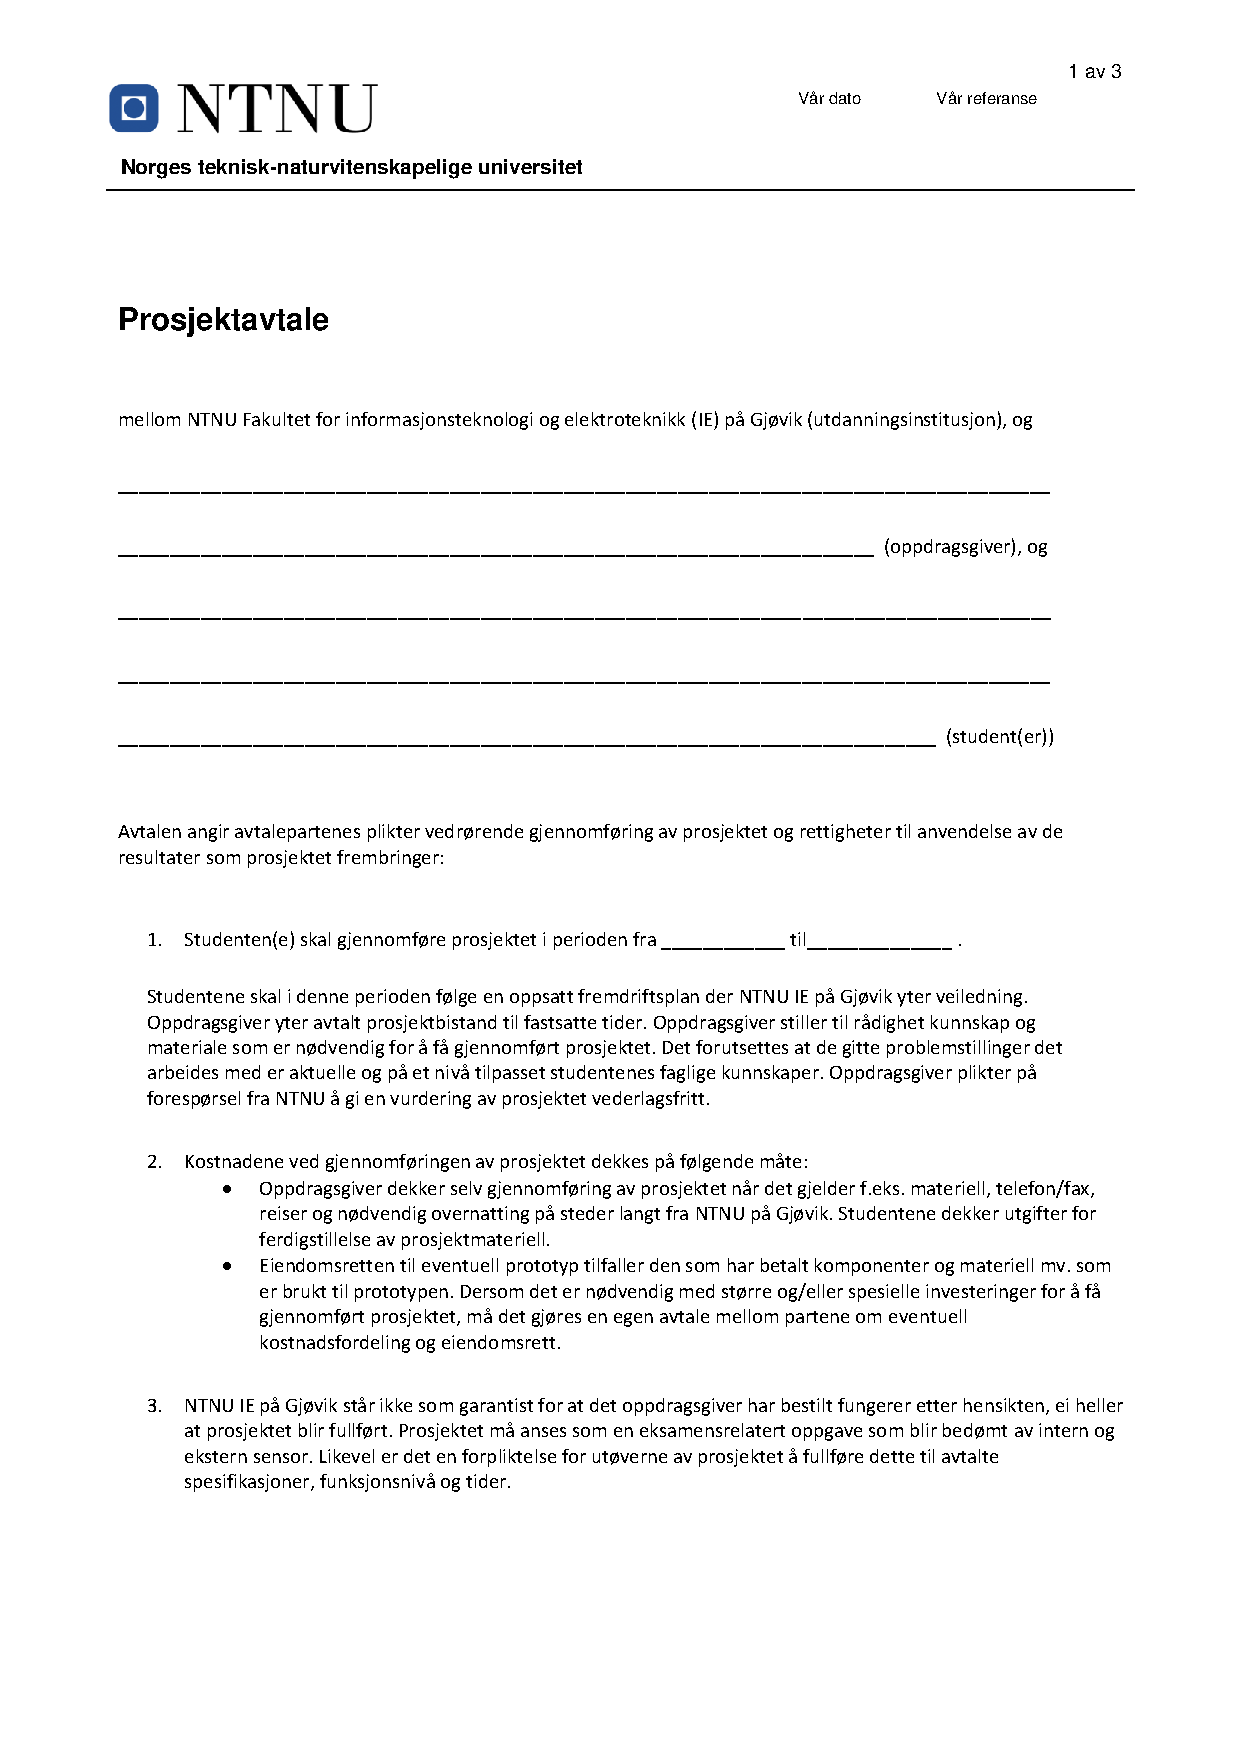
\includepdf[pages=-]{appendices/NTNUProsjektavtale.pdf}
\end{comment}







\clearpage
\section{Results}
This section presents the complete results of the experiments where some results were condensed to convey the primary findings.

\subsection{Block-NeRF}
% The full Block-NeRF evaluation table. Only the condensed version containing the average across the different segments are included in the result-section

\begin{table}[H]
\centering
\setlength{\tabcolsep}{6pt}
\renewcommand{\arraystretch}{1.5}
\begin{tabular}{l | C{2.2} C{1.3} C{1.3}}
\hline
\textbf{Description} & \textbf{PSNR $\uparrow$} & \textbf{SSIM $\uparrow$} & \textbf{LPIPS $\downarrow$} \\
\hline
Segment 1 & 24.960262 & 0.815270 & 0.161623 \\
Segment 2 & 25.660400 & 0.824085 & 0.164296 \\
Segment 3 & 23.914209 & 0.755183 & 0.194245 \\
Segment 4 & 23.363695 & 0.764547 & 0.216242 \\
\hline
\end{tabular}
\caption{Results for each segment when the baseline-segment spanning the entire block has been split into 4 Block-NeRFs.}
\label{tab:block-nerf-four-segments-full}
\end{table}


\begin{table}[H]
\centering
\setlength{\tabcolsep}{6pt}
\renewcommand{\arraystretch}{1.5}
\begin{tabular}{l | C{2.2} C{1.3} C{1.3}}
\hline
\textbf{Description} & \textbf{PSNR $\uparrow$} & \textbf{SSIM $\uparrow$} & \textbf{LPIPS $\downarrow$} \\
\hline
Segment 1 & 25.047100 & 0.826931 & 0.138852 \\
Segment 2 & \cellcolor{green} 25.703838 & 0.831167 & 0.156331 \\
Segment 3 & 24.924395 & 0.830144 & 0.149870 \\
Segment 4 & \cellcolor{red} 22.726223 & \cellcolor{red} 0.713277 & \cellcolor{red} 0.207025 \\
Segment 5 & 25.468483 & 0.837942 & \cellcolor{green} 0.131815 \\
Segment 6 & 25.670006 & \cellcolor{green} 0.841962 & 0.147232 \\
Segment 7 & 25.661350 & 0.820813 & 0.163685 \\
Segment 8 & 25.070913 & 0.777114 & 0.154277 \\
Segment 9 & 24.803871 & 0.814633 & 0.154028 \\
Segment 10 & 23.693977 & 0.753770 & 0.185557 \\
Segment 11 & 23.936722 & 0.757462 & 0.179283 \\
Segment 12 & 24.584238 & 0.807874 & 0.144022 \\
\hline
Average metrics of 12 Block-NeRF & \cellcolor{green} 24.774259 & \cellcolor{green} 0.801090 & \cellcolor{green} 0.159331 \\
Average metrics of 1 Block-NeRF & \cellcolor{red} 22.515461 & \cellcolor{red} 0.654036 & \cellcolor{red} 0.424356 \\
\hline
\end{tabular}
\caption{Results for exp\_block\_nerf\_long\_path\_2-block\_10}
\label{tab:block-nerf-twelve-segments-full}
\end{table}


\subsection{Real data} \label{app:real-data}

\begin{table}[H]
\centering
\setlength{\tabcolsep}{6pt}
\renewcommand{\arraystretch}{1.5}
\begin{tabular}{l | C{2.2} C{1.3} C{1.3} c}
\hline
\textbf{Description} & \textbf{PSNR $\uparrow$} & \textbf{SSIM $\uparrow$} & \textbf{LPIPS $\downarrow$} & \textbf{Time processing} \\
\hline
COLMAP w/ optimizer           & 19.937267 & 0.723673 & 0.534969 & 00:10:25 \\
COLMAP w/o optimizer          & 20.990921 & 0.757042 & 0.467530 & 00:10:25 \\
COLMAP w/ optimizer, 4 BNs    & 20.365336 & 0.75952125 & 0.427666 & 00:10:25 \\
COLMAP w/o optimizer, 4 BNs   & 20.45474375 & 0.761062 & 0.4253 & 00:10:25 \\
GPS w/ optimizer              & 18.877967 & 0.710520 & 0.573053 & 00:00:00 \\
GPS w/o optimizer             & 15.288701 & 0.692639 & 0.649337 & 00:00:00 \\
GPS w/ optimizer, 4 BNs       & 18.4146345 & 0.69007725 & 0.560061 & 00:00:00 \\
GPS w/o optimizer, 4 BNs      & 14.578463 & 0.6671365 & 0.65638525 & 00:00:00 \\
\hline
\end{tabular}
\caption{Data from Trip088 with transformation matrix approximated with COLMAP or GPS-readings. BNs an abbreviation of Block-NeRF and the resulting metric score is averaged across the 4 NeRFs evaluations.}
\label{tab:trip088-results}
\end{table}

\begin{table}[H]
\centering
\setlength{\tabcolsep}{6pt}
\renewcommand{\arraystretch}{1.5}
\begin{tabular}{l | C{2.2} C{1.3} C{1.3} c}
\hline
\textbf{Description} & \textbf{PSNR $\uparrow$} & \textbf{SSIM $\uparrow$} & \textbf{LPIPS $\downarrow$} & \textbf{Time processing} \\
\hline
COLMAP w/ optimizer           & 19.839231 & 0.681580 & 0.542084 & 00:08:45 \\
COLMAP w/o optimizer          & 22.312044 & 0.751723 & 0.431454 & 00:08:45 \\
COLMAP w/ optimizer, 4 BNs    & 20.97288575 & 0.6987495 & 0.3971635 & 00:08:45 \\
COLMAP w/o optimizer, 4 BNs    & 23.39594125 & 0.794048 & 0.32915525 & 00:08:45 \\
GPS w/ optimizer              & 18.165668 & 0.653362 & 0.597592 & 00:00:00 \\
GPS w/o optimizer             & 13.796535 & 0.626601 & 0.719307 & 00:00:00 \\
GPS w/ optimizer, 4 BNs       & 18.401476 & 0.6379955 & 0.5449655 & 00:00:00 \\
GPS w/o optimizer, 4 BNs       & 14.37125725 & 0.6192 & 0.68332825 & 00:00:00 \\
\hline
\end{tabular}
\caption{Data from Trip094 with transformation matrix approximated with COLMAP or GPS-readings. BNs an abbreviation of Block-NeRF and the resulting metric score is averaged across the 4 NeRFs evaluations.}
\label{tab:trip094-results}
\end{table}

% Not sure if I should include the results for Trip067 as it hasn't been introduced as a dataset
\begin{comment}
\begin{table}[ht]
\centering
\setlength{\tabcolsep}{6pt}
\renewcommand{\arraystretch}{1.5}
\begin{tabular}{l | C{2.2} C{1.3} C{1.3} c}
\hline
\textbf{Description} & \textbf{PSNR $\uparrow$} & \textbf{SSIM $\uparrow$} & \textbf{LPIPS $\downarrow$} & \textbf{Time processing} \\
\hline
COLMAP w/ optimizer           & 23.486408   & 0.864474 & 0.421610 & 01:05:59 \\
COLMAP w/o optimizer          & 22.640327   & 0.865871 & 0.401821 & 01:05:59 \\
COLMAP w/ optimizer, 12 BNs   &\cellcolor{green} 25.65282775 &\cellcolor{green} 0.882313 &\cellcolor{green} 0.332909 & 01:05:59 \\
GPS w/ optimizer              & 21.741020   & 0.849057 & 0.422538 & 00:00:00 \\
GPS w/o optimizer             &\cellcolor{red} 21.625042   &\cellcolor{red} 0.847604 &\cellcolor{red} 0.422631 & 00:00:00 \\
GPS w/ optimizer, 12 BNs      & 22.65892333 & 0.848332 & 0.393478 & 00:00:00 \\
\hline
\end{tabular}
\caption{Data from Trip067 with transformation matrix approximated with COLMAP or GPS-readings. BNs an abbreviation of Block-NeRF and the resulting metric score is averaged across the 12 NeRFs evaluations.}
\label{tab:trip067-results}
\end{table}
\end{comment}

\subsection{Adding noise} \label{app:noise}
\begin{table}[H]
\centering
\setlength{\tabcolsep}{6pt}
\renewcommand{\arraystretch}{1.5}
\begin{tabular}{l | C{2.2} C{1.3} C{1.3} | C{2.2} C{1.3} C{1.3}}
\hline
\textbf{Description} & \textbf{PSNR $\uparrow$} & \textbf{SSIM $\uparrow$} & \textbf{LPIPS $\downarrow$} & \textbf{PSNR $\uparrow$} & \textbf{SSIM $\uparrow$} & \textbf{LPIPS $\downarrow$} \\
\hline
& \multicolumn{6}{c}{\textbf{Baseline segment}} \\
\hline
& \multicolumn{3}{c}{\textbf{With camera optimizer}} & \multicolumn{3}{c}{\textbf{Without camera optimizer}} \\
\hline
$\mathcal{N}(0, 0.0)$   & 23.412970 & 0.713507 & 0.320640 & 24.702831 & 0.792646 & 0.179289 \\
$\mathcal{N}(0, 0.1^2)$ & 22.513981 & 0.674136 & 0.321364 & 22.463675 & 0.677371 & 0.280633 \\
$\mathcal{N}(0, 0.2^2)$ & 21.343519 & 0.616709 & 0.338266 & 21.212559 & 0.601917 & 0.366598 \\
$\mathcal{N}(0, 0.3^2)$ & 20.520330 & 0.577203 & 0.345663 & 20.468809 & 0.560959 & 0.399360 \\
$\mathcal{N}(0, 0.5^2)$ & 19.075649 & 0.501499 & 0.371572 & 19.366894 & 0.499264 & 0.474444 \\
$\mathcal{N}(0, 1.0^2)$ & 17.670620 & 0.433909 & 0.432940 & 18.207266 & 0.444120 & 0.560452 \\
$\mathcal{N}(0, 3.0^2)$ & 16.662760 & 0.408036 & 0.637326 & 16.322678 & 0.385614 & 0.647966 \\
\hline
& \multicolumn{6}{c}{\textbf{Shorter segment}} \\
\hline
& \multicolumn{3}{c}{\textbf{With camera optimizer}} & \multicolumn{3}{c}{\textbf{Without camera optimizer}} \\
\hline
$\mathcal{N}(0, 0.0)$   & 24.831890 & 0.824606 & 0.102266 & 25.677803 & 0.861634 & 0.076989 \\ 
$\mathcal{N}(0, 0.1^2)$ & 23.028709 & 0.752731 & 0.114806 & 23.318026 & 0.755237 & 0.146877 \\ 
$\mathcal{N}(0, 0.2^2)$ & 20.674553 & 0.613583 & 0.148965 & 21.383156 & 0.628668 & 0.209283 \\ 
$\mathcal{N}(0, 0.3^2)$ & 20.502602 & 0.595552 & 0.154787 & 21.101936 & 0.612378 & 0.232985 \\ 
$\mathcal{N}(0, 0.5^2)$ & 19.059755 & 0.482721 & 0.197262 & 20.071671 & 0.513037 & 0.299472 \\ 
$\mathcal{N}(0, 1.0^2)$ & 18.085838 & 0.406564 & 0.338364 & 18.290358 & 0.417969 & 0.404933 \\ 
$\mathcal{N}(0, 3.0^2)$ & 15.709220 & 0.344876 & 0.612587 & 15.077240 & 0.362973 & 0.698665 \\ 
\hline
\end{tabular}
\caption{Results for Gaussian Noise experiment on both the baseline and shorter segments. The shorter segments are 10\% the size of the baseline segment, approximately 50m in length.}
\label{tab:exp-gaussian-noise-full}
\end{table}

\end{document}
